\documentclass[a4paper,12pt]{report}
\usepackage[T1]{fontenc}
\usepackage[utf8]{inputenc}
\usepackage{lmodern}
\usepackage{epsfig,wrapfig}
%\usepackage{epsfig,wrapfig}
\usepackage{pdfpages}

\oddsidemargin3.cm
\evensidemargin3.cm
\textheight=22cm
\textwidth=15.0cm
\topmargin=-2mm
\hoffset= -2.5cm
\voffset= -0.5cm


\begin{document}
{\LARGE \bf Single-Energy fits of MAID2015a pseudodata}
~\\
~\\

\large
I did several single energy fits with the MAID2015a pseudodata with
different constraints and starting values. In all cases I just fitted
the 4 observables: $d\sigma/d\Omega$, $\Sigma$, $T$ and $F$. For these 
observables we already have experimental data. This set is not complete
and we might expect ambiguities.  
\paragraph{1. Unconstrained fit with MAID2015a starting values} 
~\\
In this fit up to H-waves ($\ell = 6$) 40 parameters were fitted. Fig.~\ref{Fig:free1} shows
the results for the s-,-p, and d-waves. The lines show the MAID15a ("true") solution. 
The starting parameters of the fit were randomly selected in a 50\% range relative to 
the "true" solution.

\paragraph{2. Unconstrained fit with BnGa starting values} 
~\\
Here, the same fit was repeated. Only the starting parameters of the fit were 
randomly selected in a 50\% range relative to a BnGa solution.
Fig.~\ref{Fig:free2} shows the results. The solid lines show the BnGa solution 
(starting values) the dashed lines the MAID2015a ("true") solution. 


\paragraph{3. Fits using the exact helicity amplitudes as constraint}
~\\
Figs.~\ref{Fig:const1} to \ref{Fig:const3} show fits of MAID2015a pseudo-data
with MAID2015a, BnGa and $\eta$-MAID2003
as starting values. Here, the squared deviation between the fitted and the MAID2015a 
helicity amplitudes averaged over the angular distribution 
was added as a penalty factor in the $\chi^2$ with weighting factor $Q = 1$.

\paragraph{4. Fits using Hedims helicity amplitudes as constraint}
~\\
As last step, I replaced the exact helictiy amplitudes by the results from 
Hedim's fixed-t analysis (Helcon-SE.dat). Figs.~ref{Fig:const4} to \ref{Fig:const6} 
show the results with starting values from MAID2015a, BnGa, and $\eta-MAID2003$.


\begin{figure}
  \begin{center}
    \centerline{
    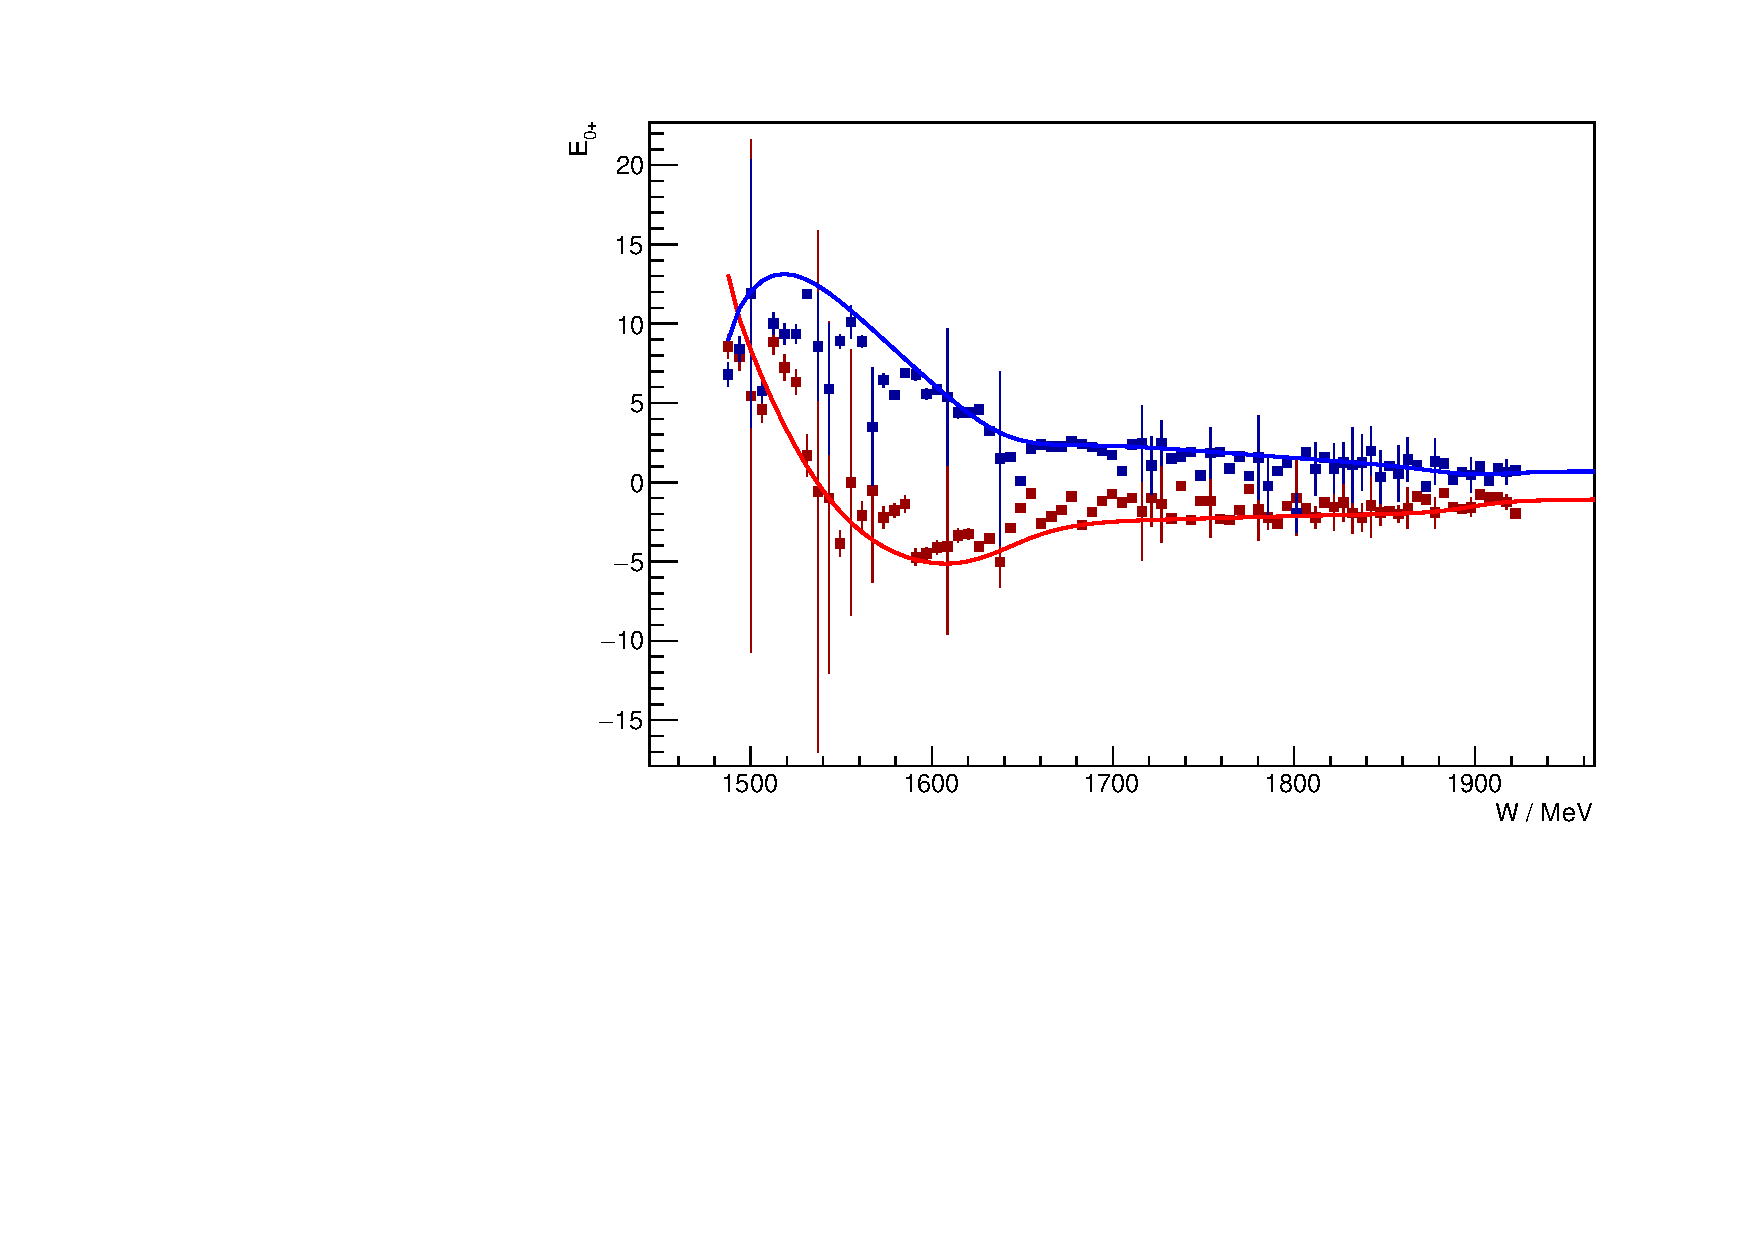
\includegraphics[width=0.49\textwidth]{MAID2015a/free/plots.0/E0p.pdf}
    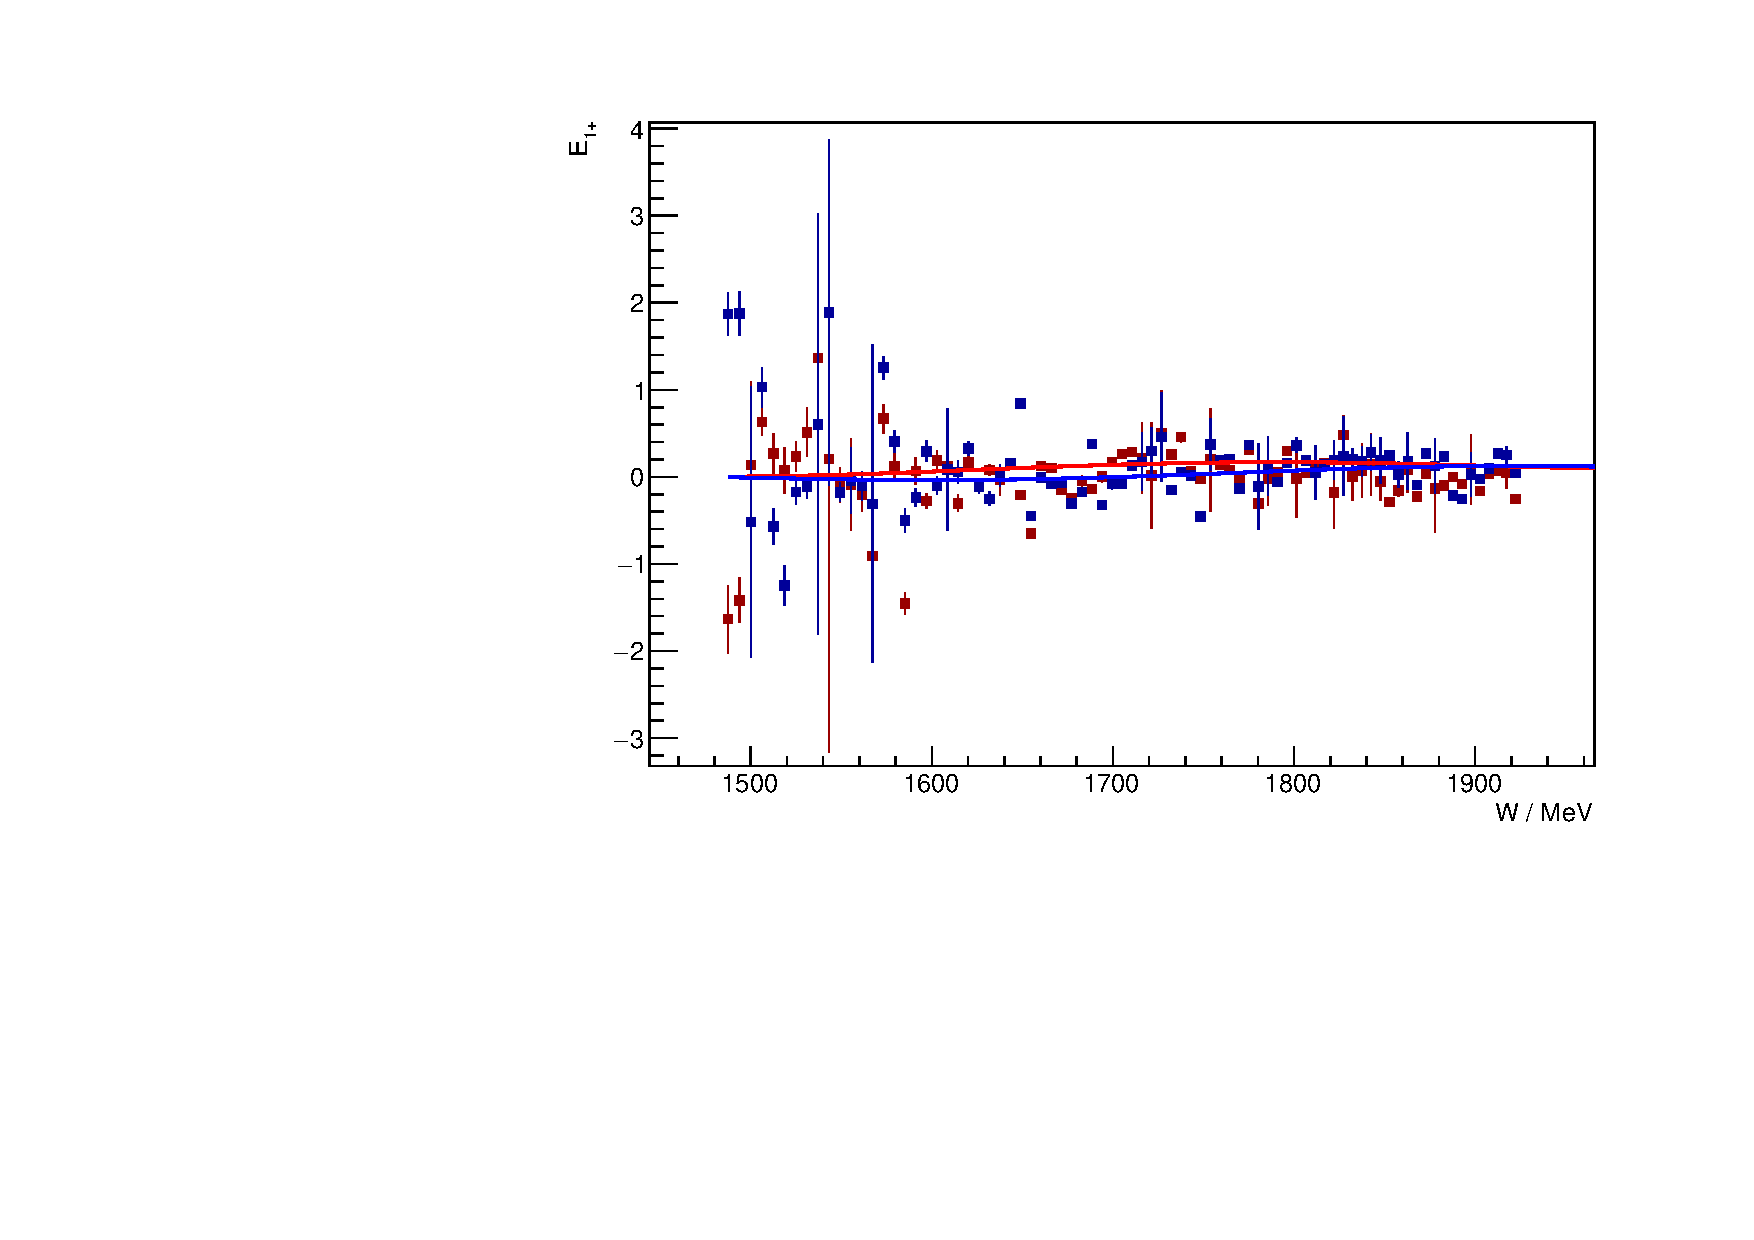
\includegraphics[width=0.49\textwidth]{MAID2015a/free/plots.0/E1p.pdf}
    }
    \centerline{
    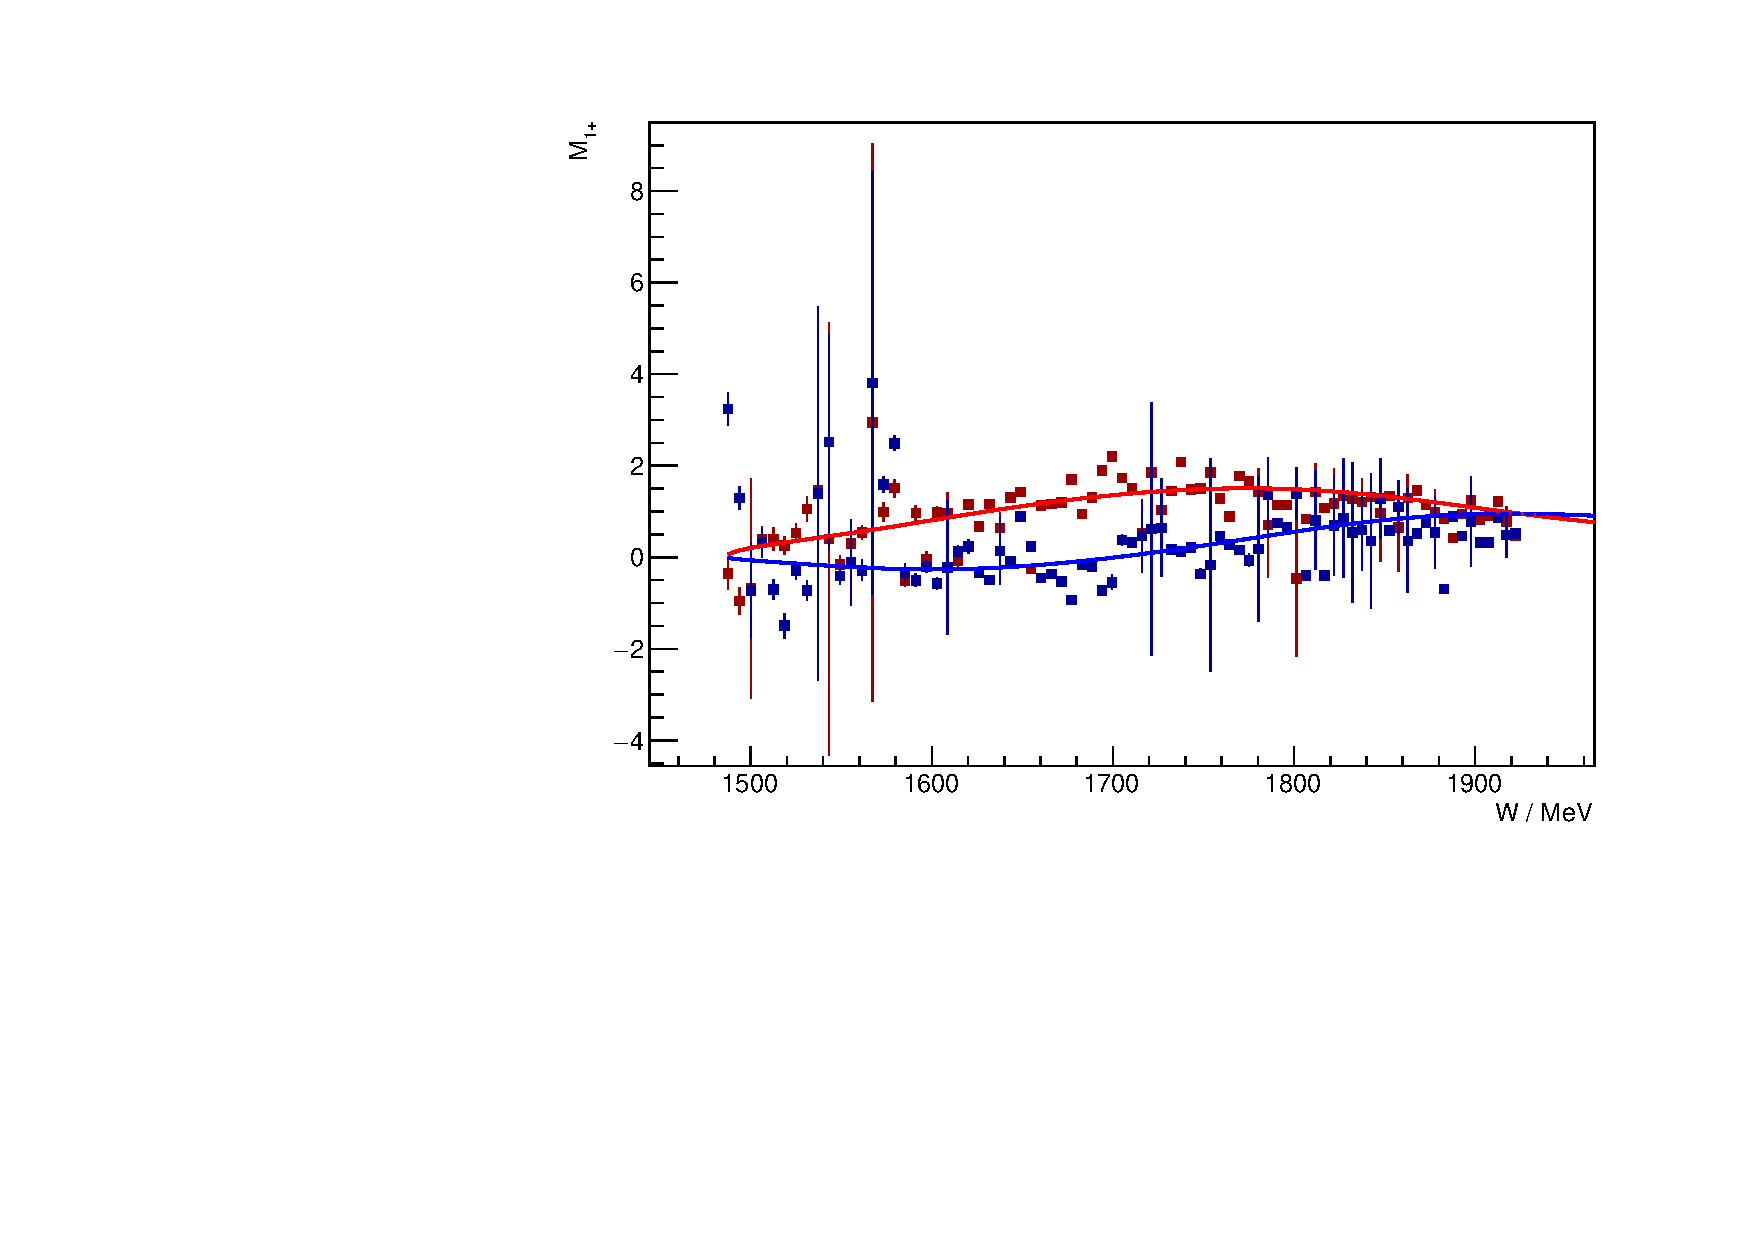
\includegraphics[width=0.49\textwidth]{MAID2015a/free/plots.0/M1p.pdf}
    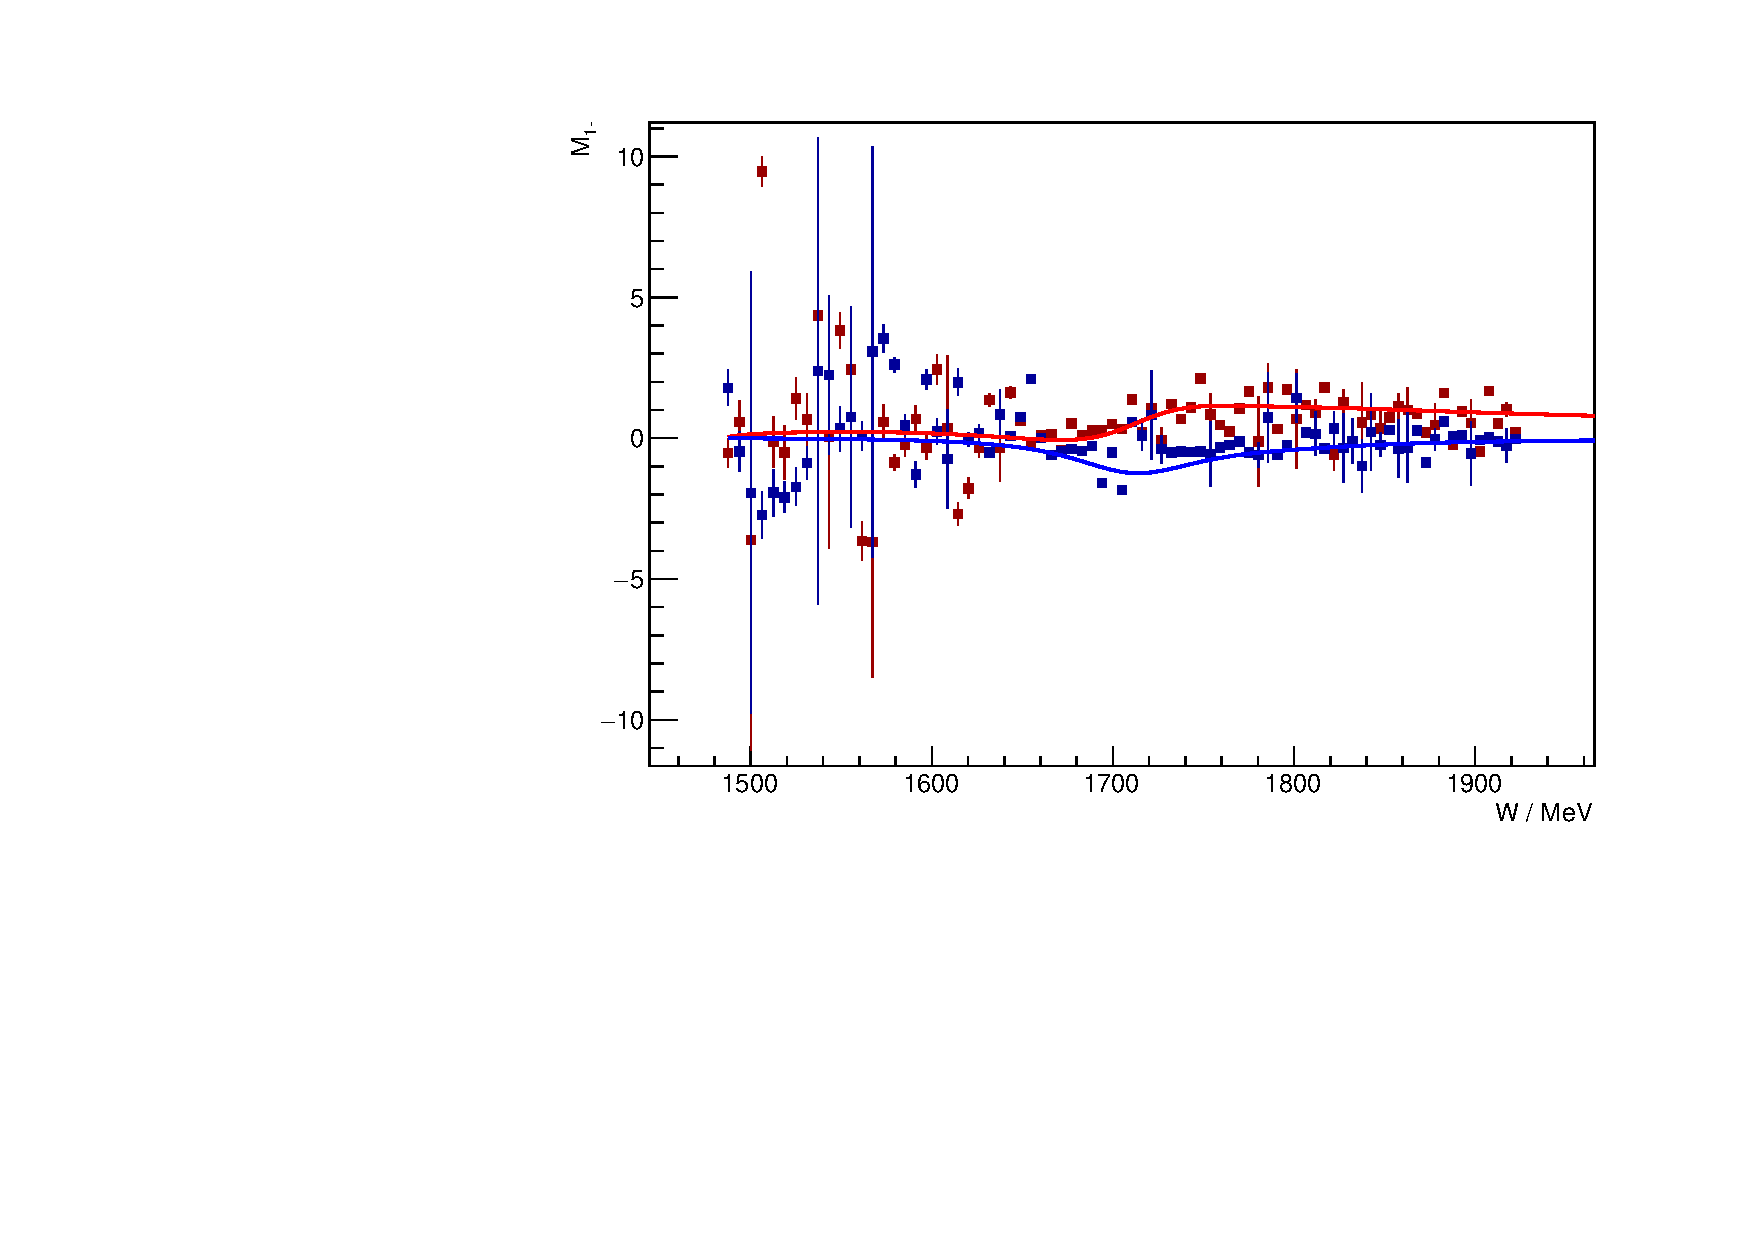
\includegraphics[width=0.49\textwidth]{MAID2015a/free/plots.0/M1m.pdf}
    }
    \centerline{
    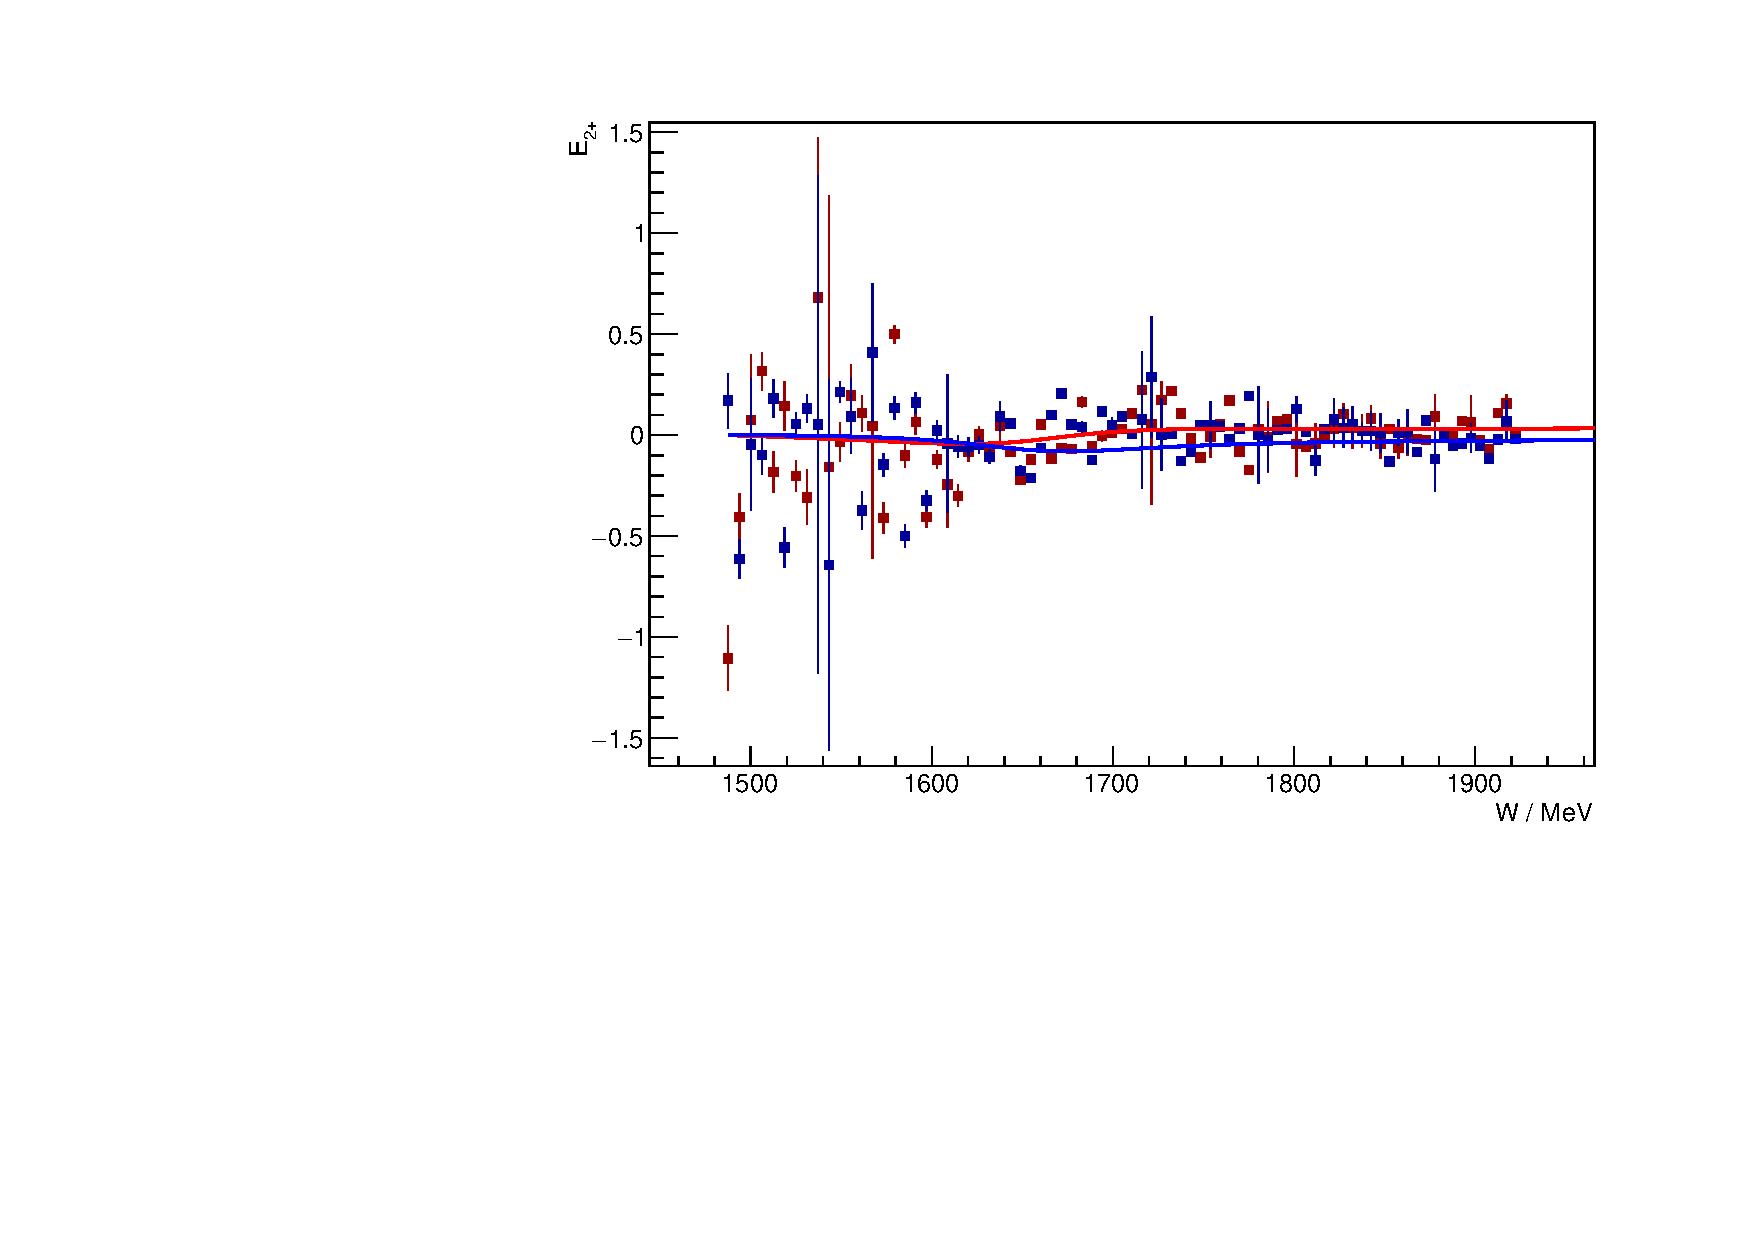
\includegraphics[width=0.49\textwidth]{MAID2015a/free/plots.0/E2p.pdf}
    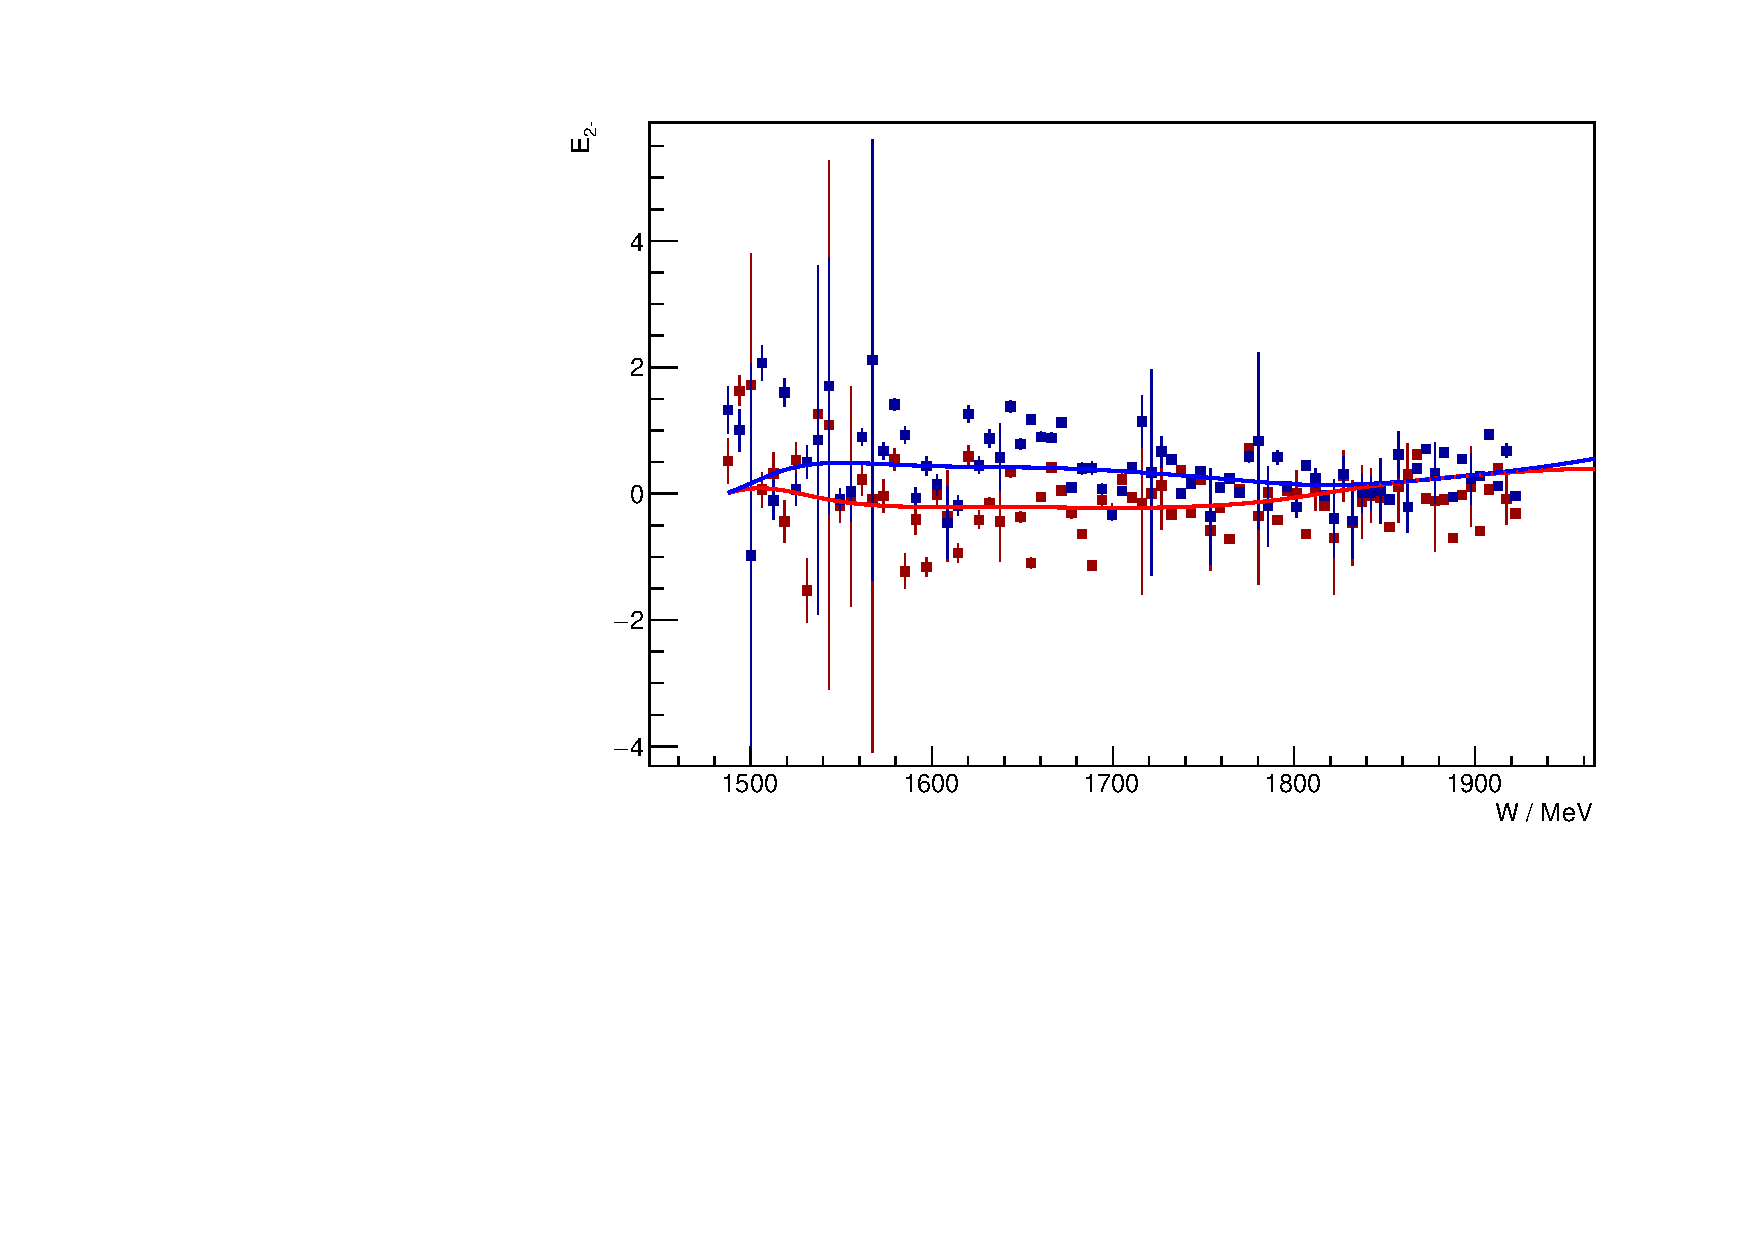
\includegraphics[width=0.49\textwidth]{MAID2015a/free/plots.0/E2m.pdf}
    }
    \centerline{
    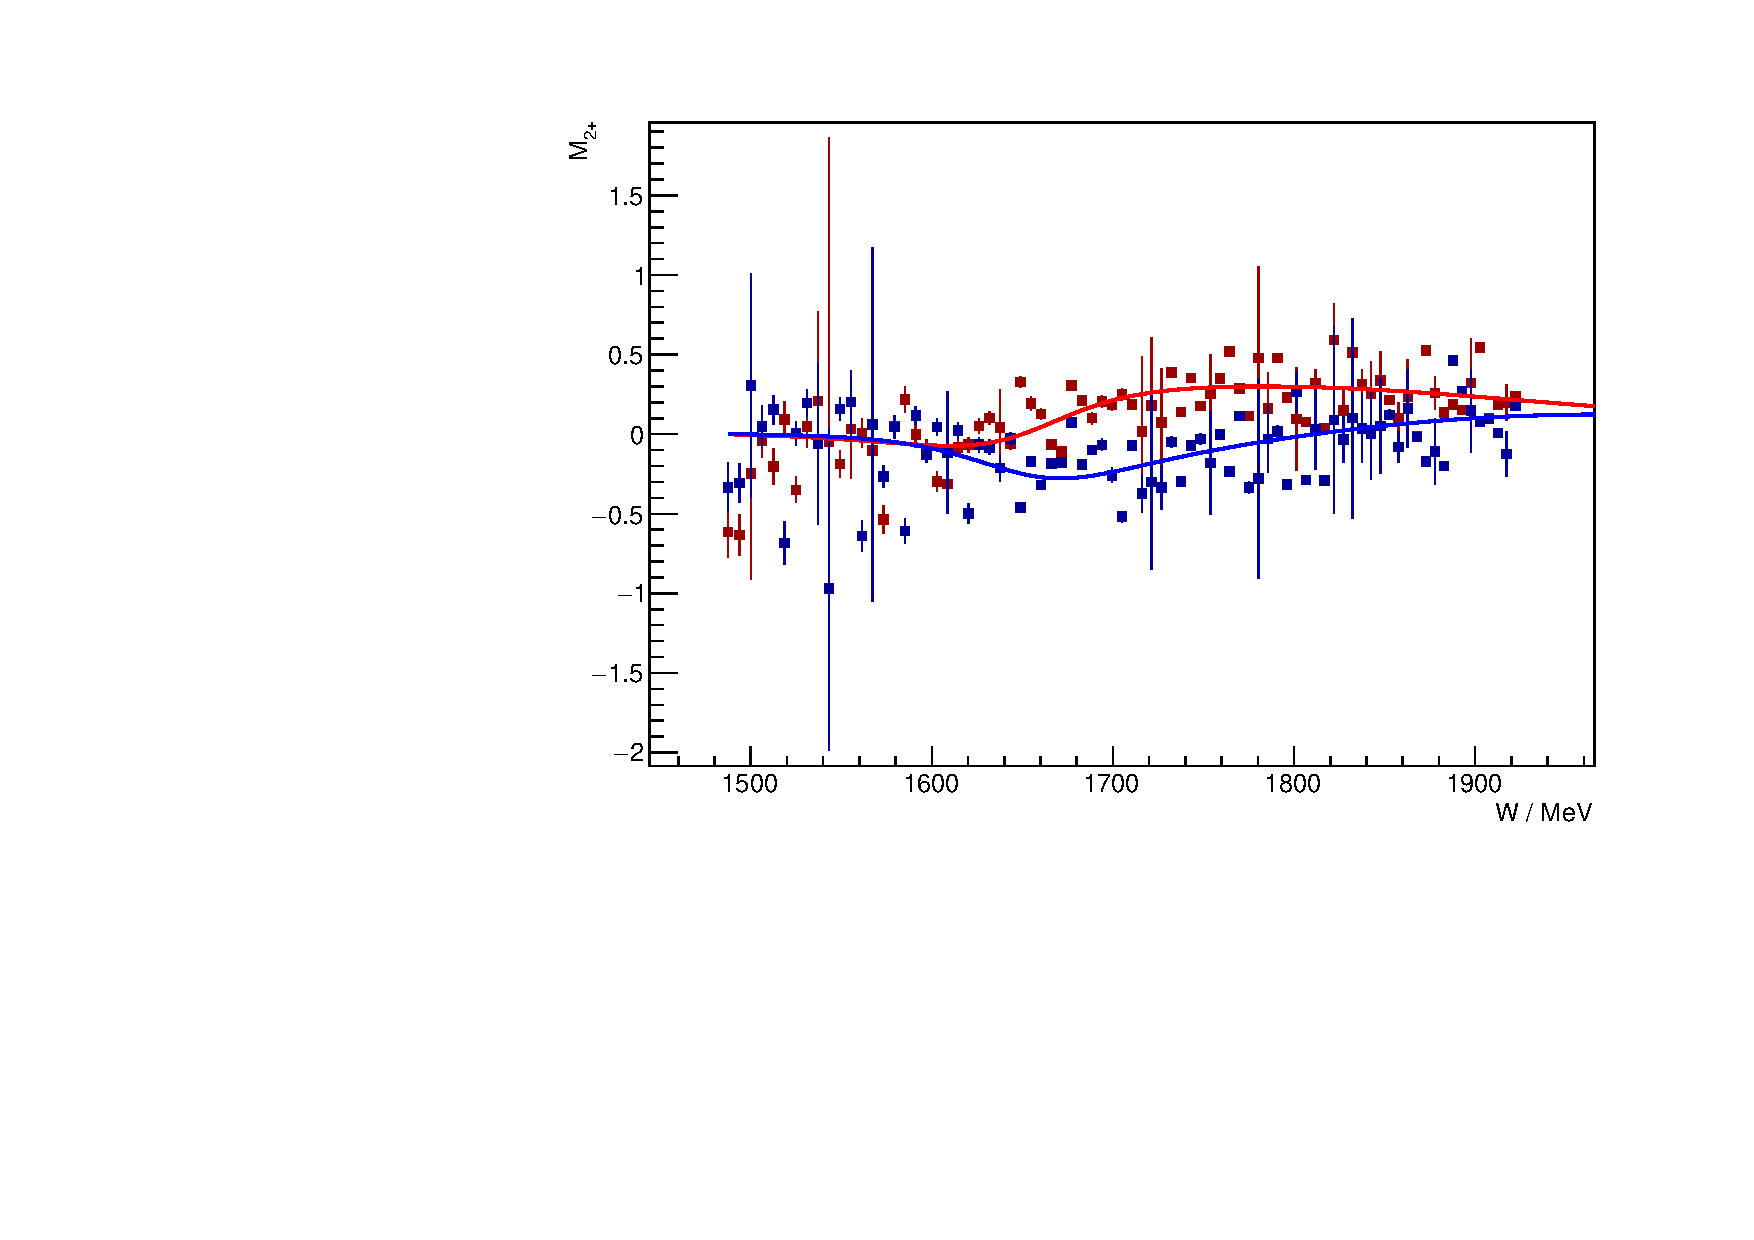
\includegraphics[width=0.49\textwidth]{MAID2015a/free/plots.0/M2p.pdf}
    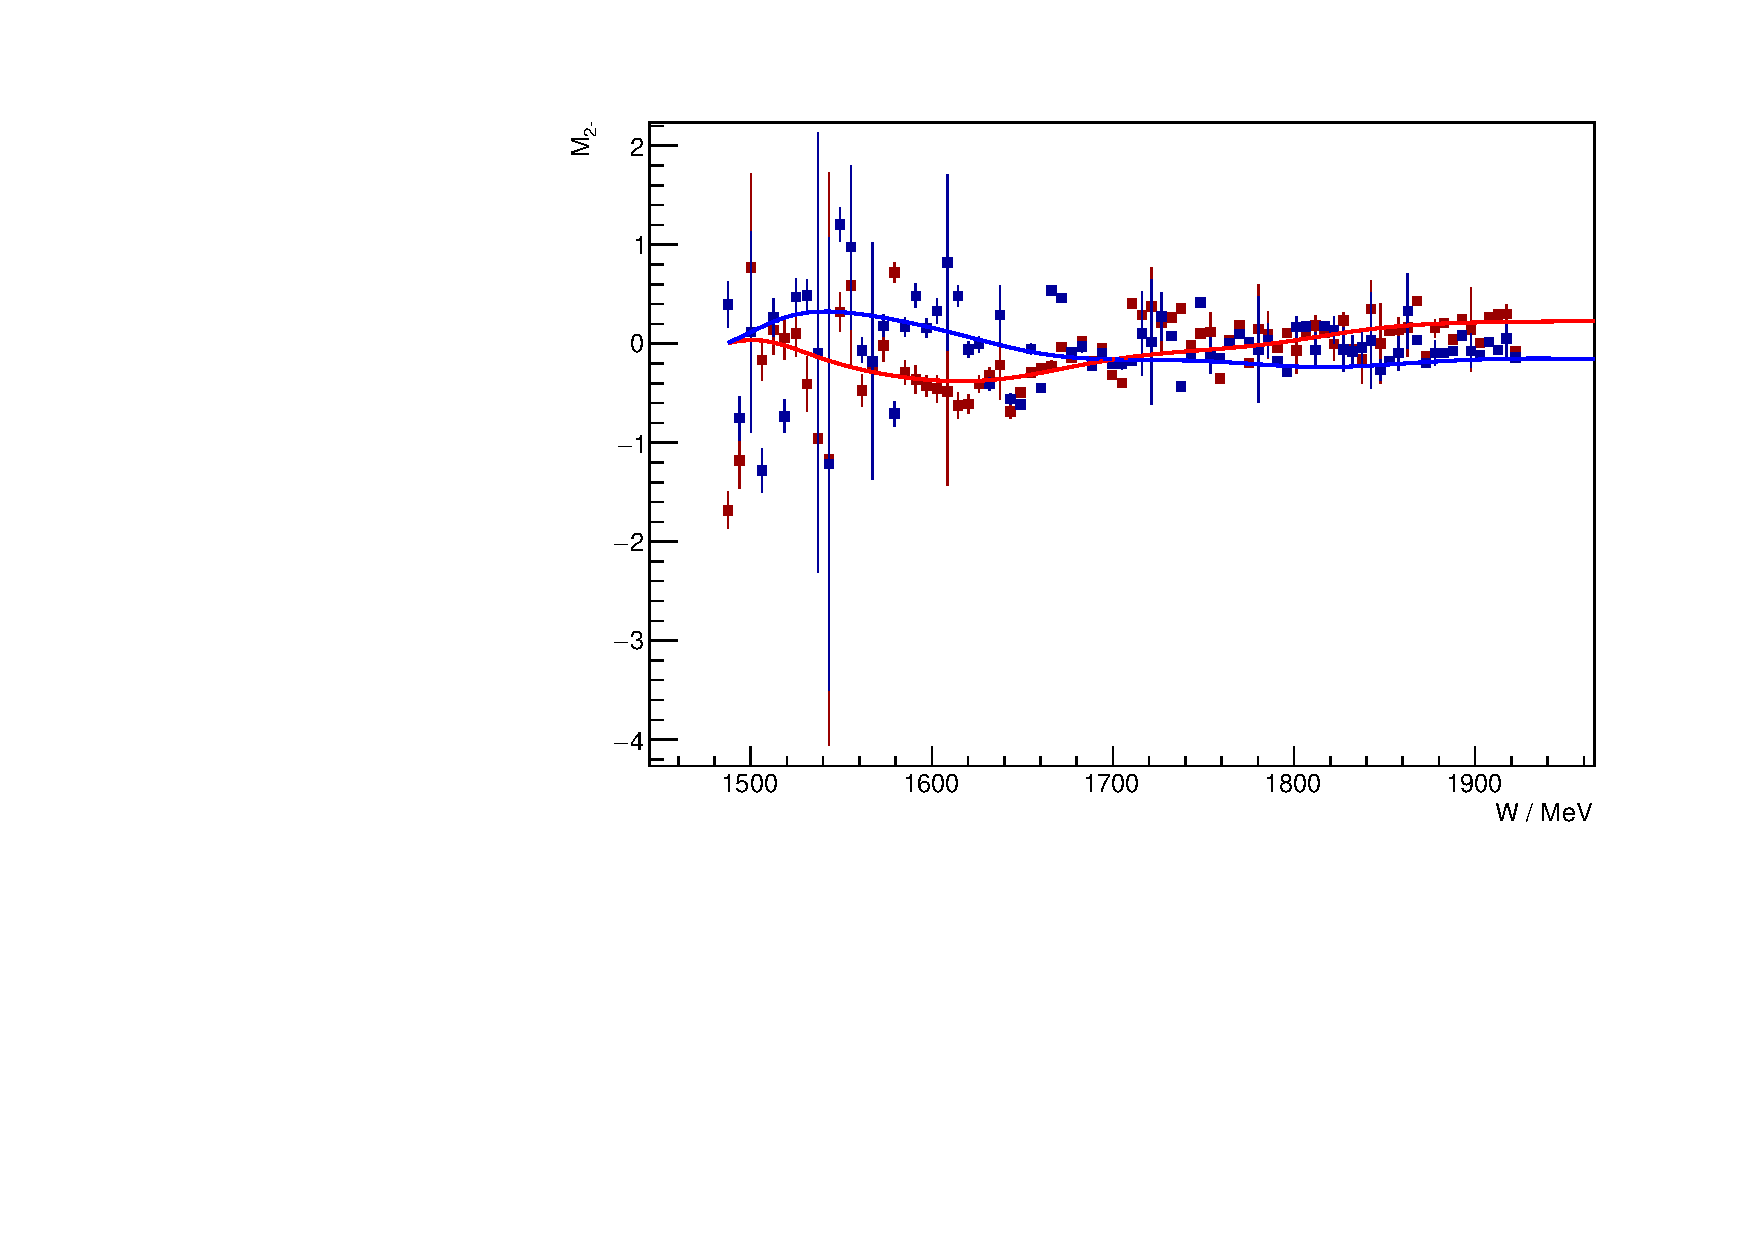
\includegraphics[width=0.49\textwidth]{MAID2015a/free/plots.0/M2m.pdf}
    }
    \caption{s-, p- and d-wave multipoles from an unconstrained fit. Red: Real-Part; Blue Im-Part.
    The lines show the MAID15a ("true") solution. The starting parameters of the fit were randomly selected 
    in a 50\% range relative to these "true" values.}
\label{Fig:free1}
  \end{center}
\end{figure}

\begin{figure}
  \begin{center}
    \centerline{
    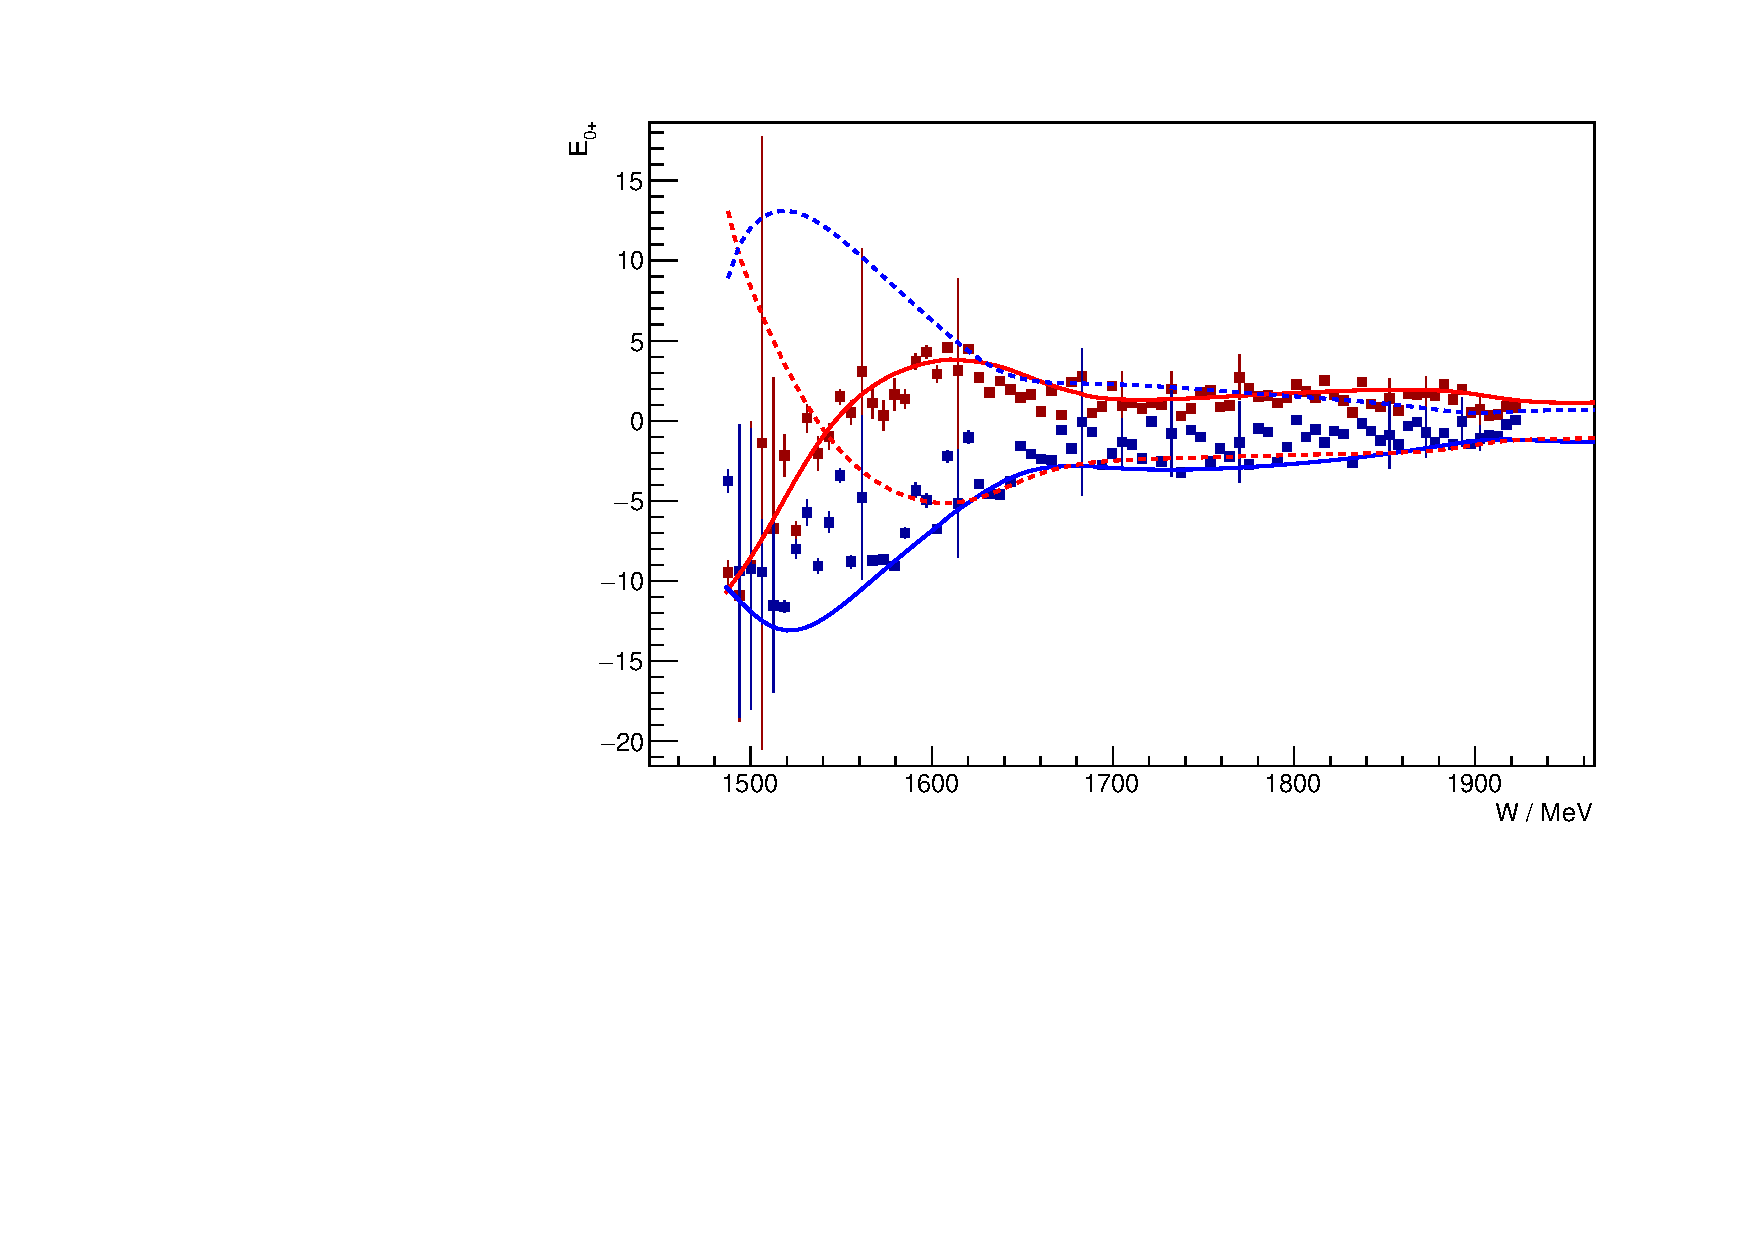
\includegraphics[width=0.49\textwidth]{BnGa/free/plots.0/E0p.pdf}
    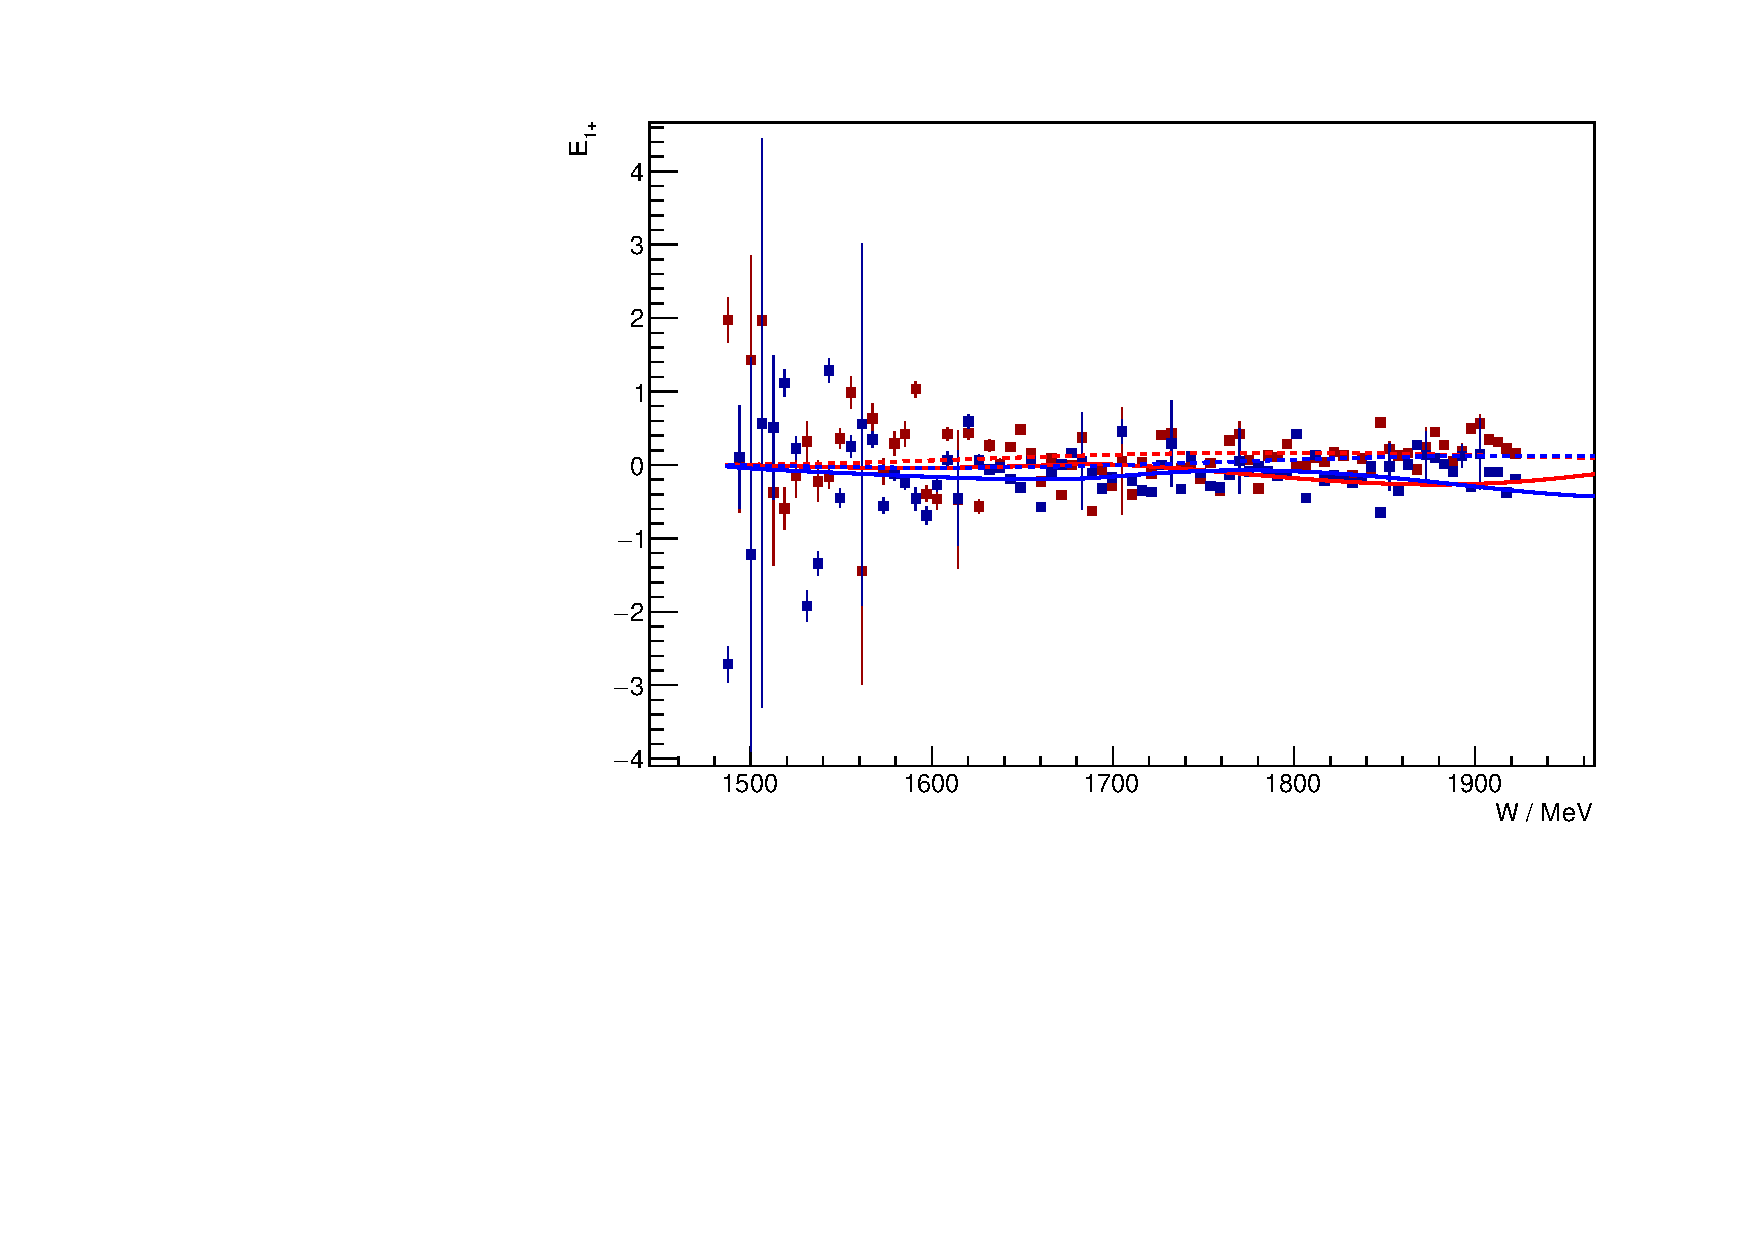
\includegraphics[width=0.49\textwidth]{BnGa/free/plots.0/E1p.pdf}
    }
    \centerline{
    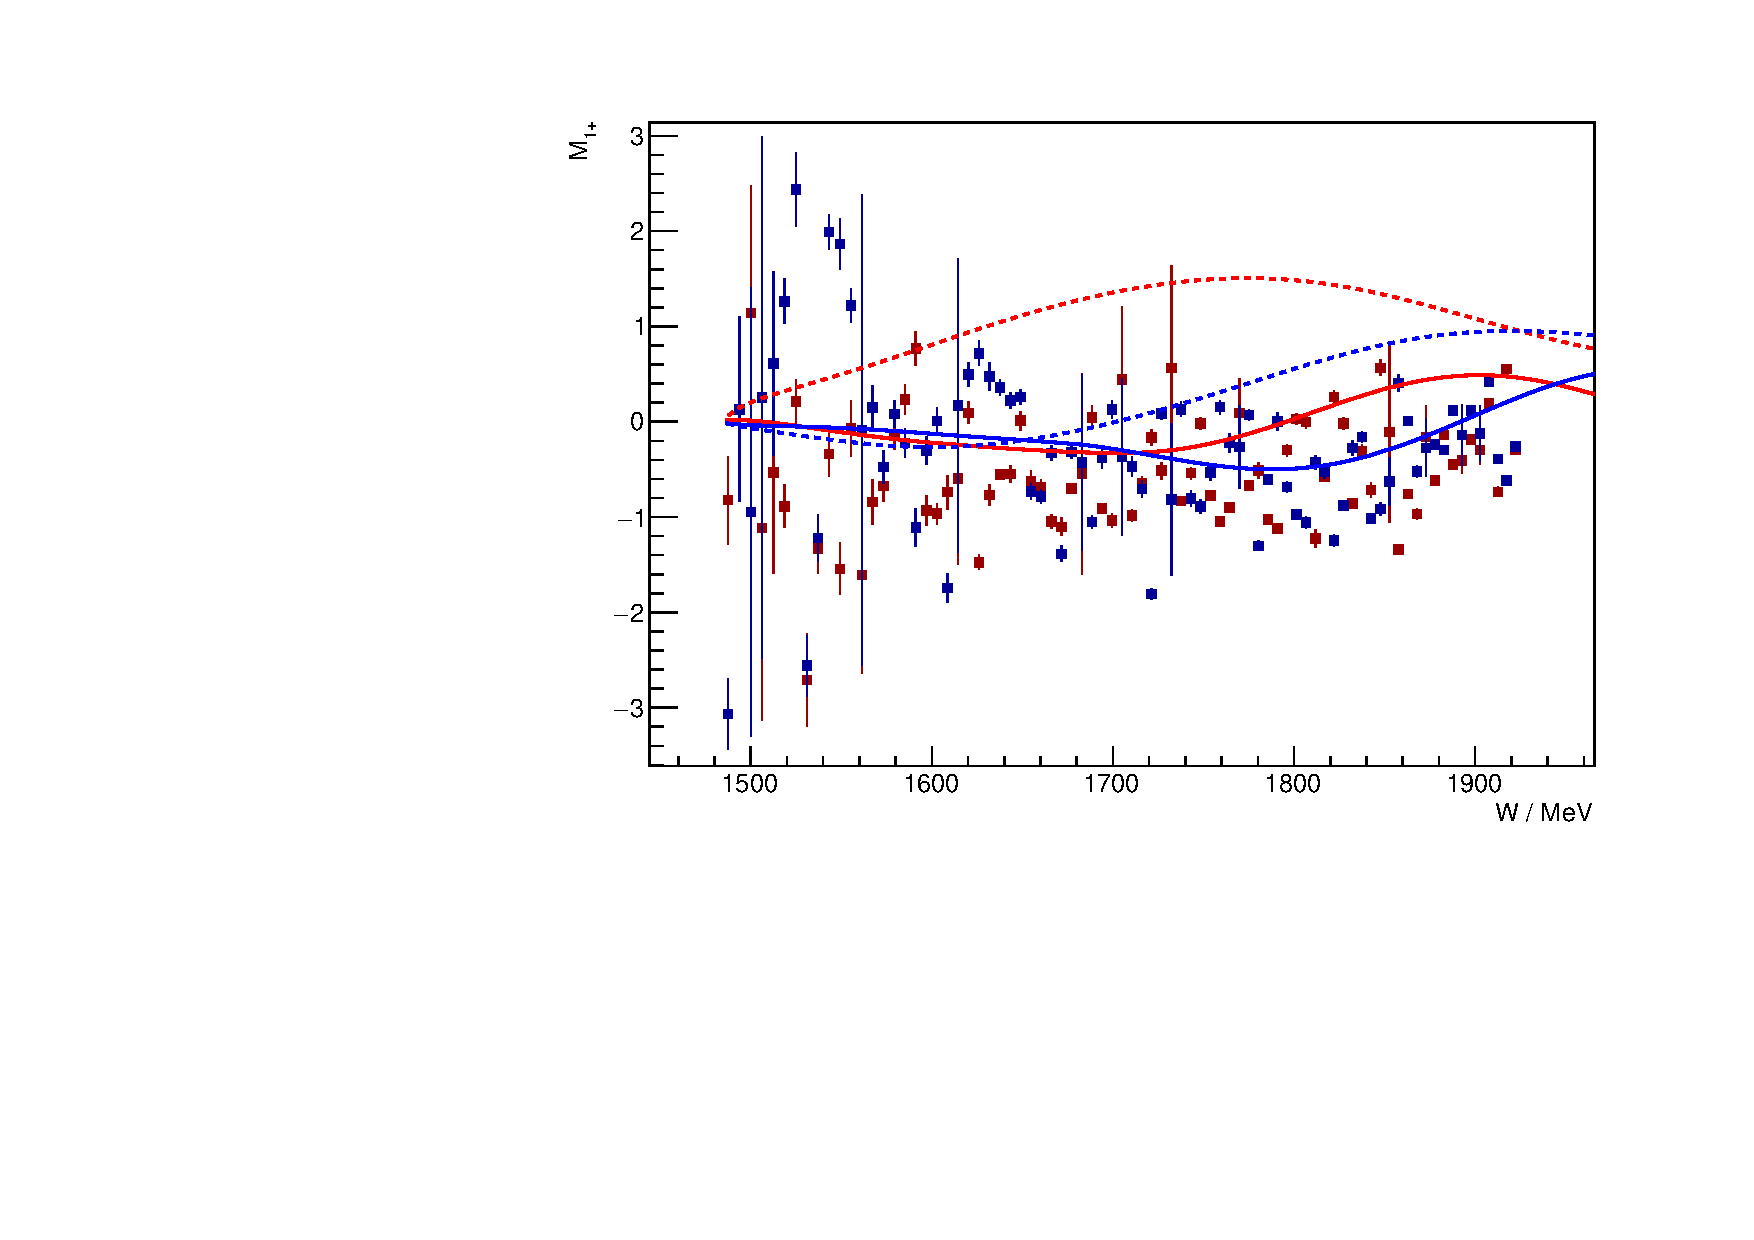
\includegraphics[width=0.49\textwidth]{BnGa/free/plots.0/M1p.pdf}
    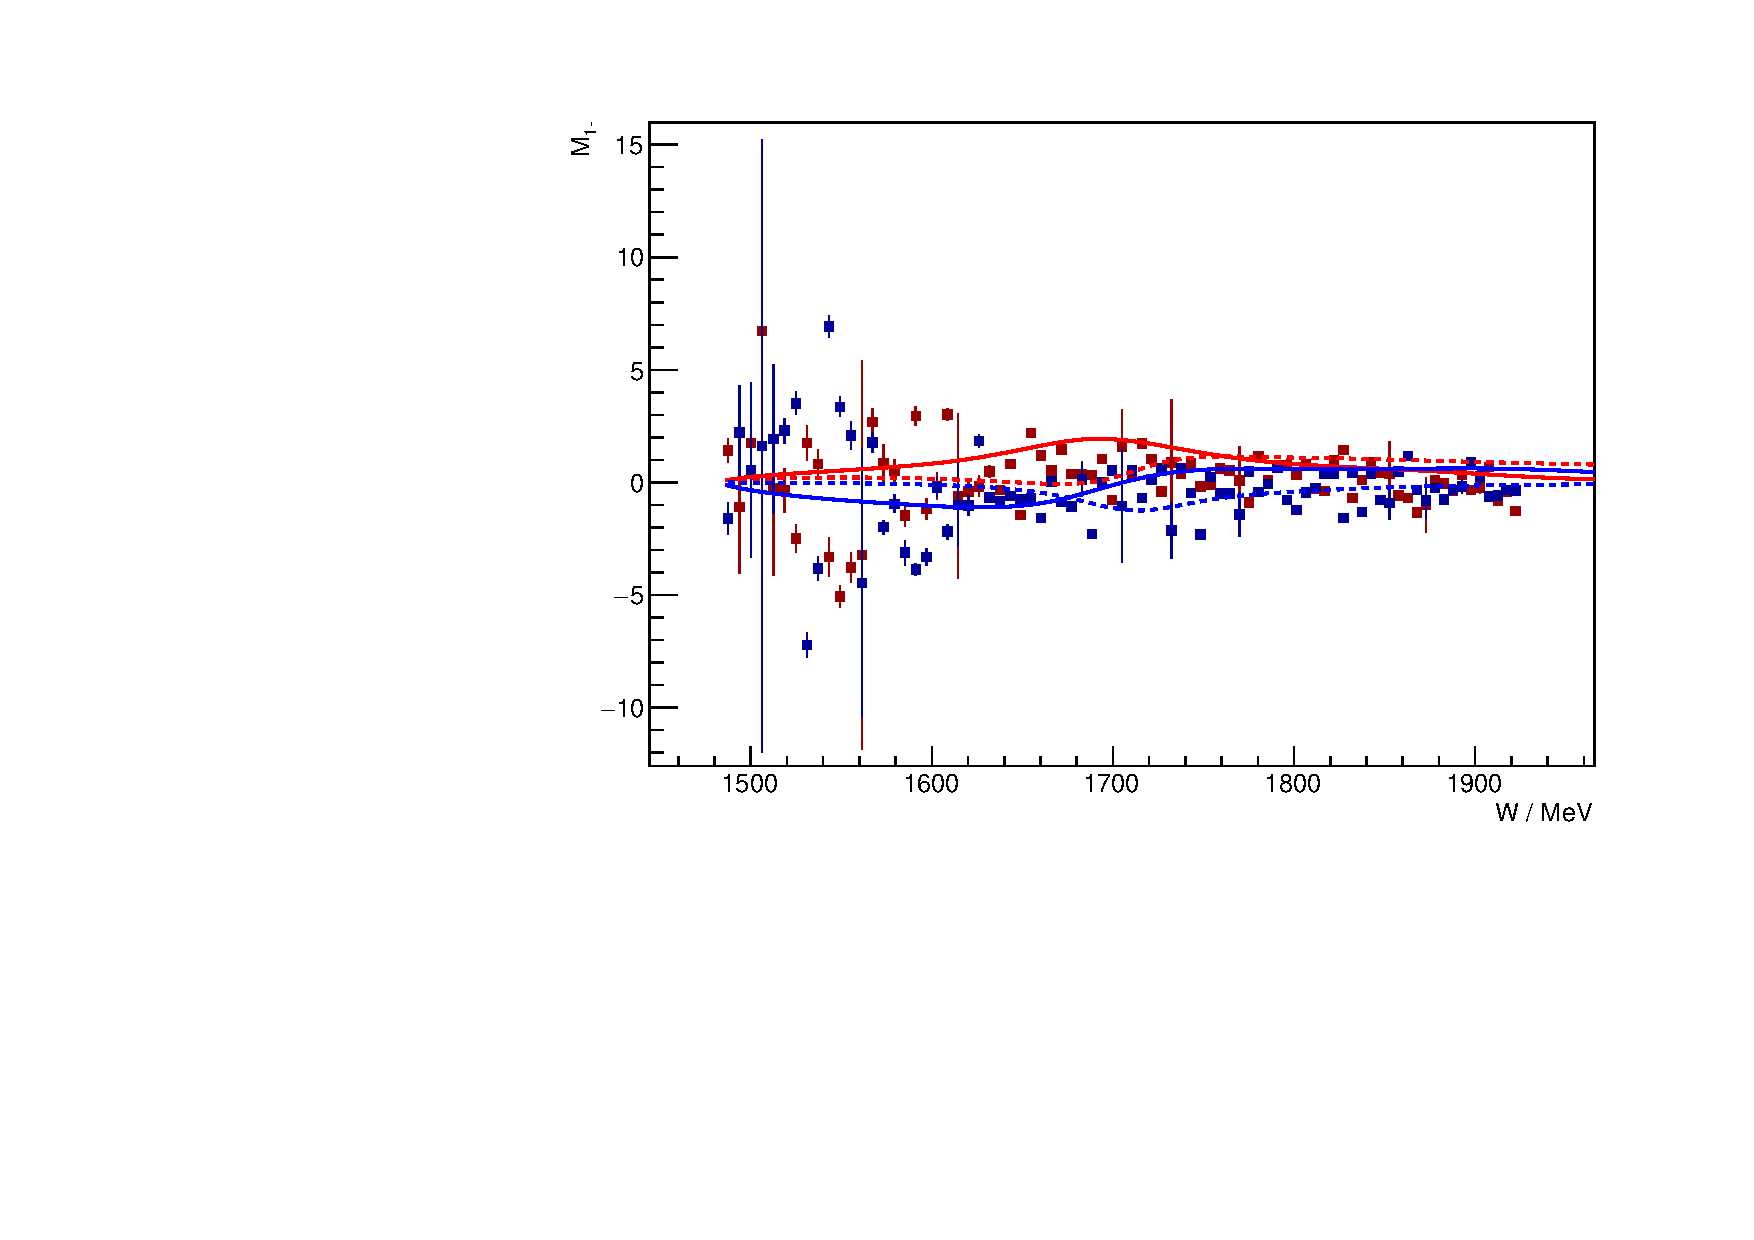
\includegraphics[width=0.49\textwidth]{BnGa/free/plots.0/M1m.pdf}
    }
    \centerline{
    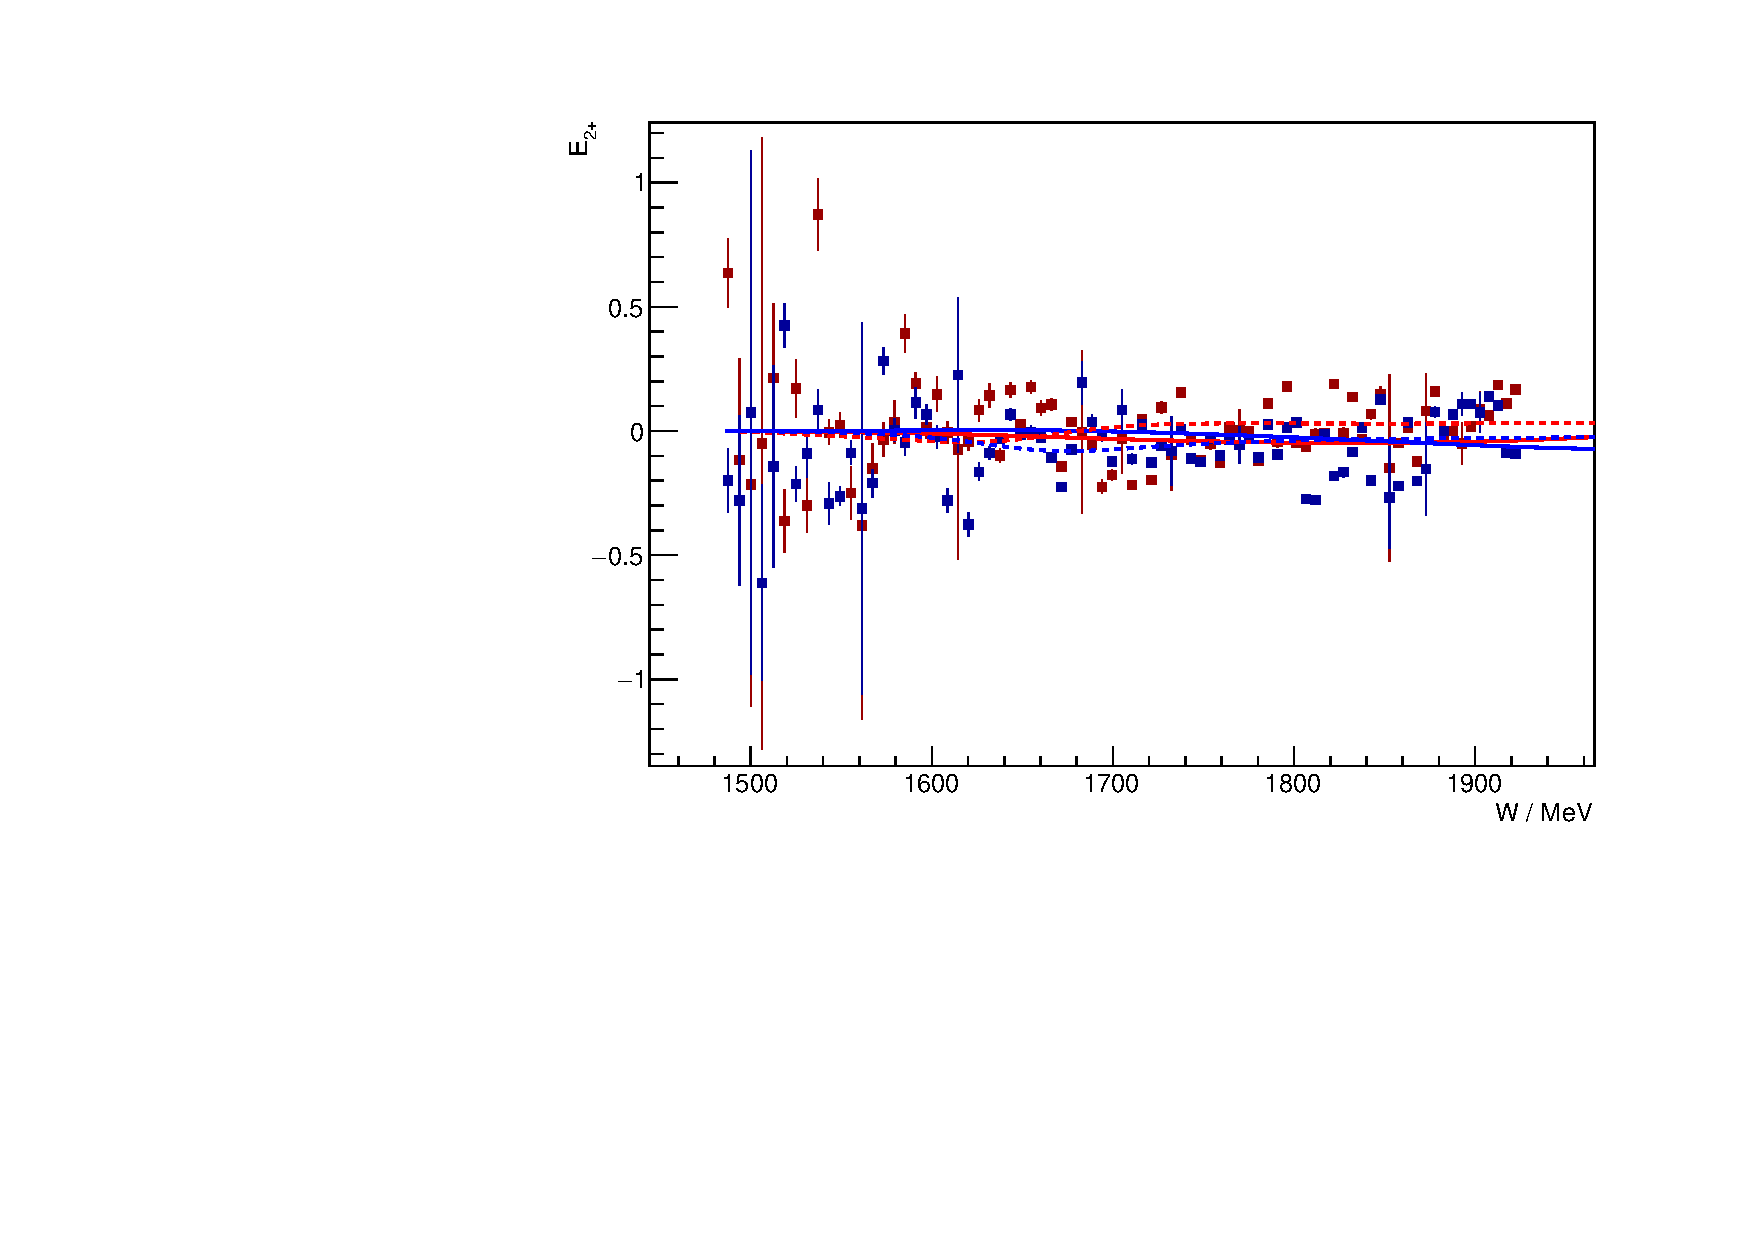
\includegraphics[width=0.49\textwidth]{BnGa/free/plots.0/E2p.pdf}
    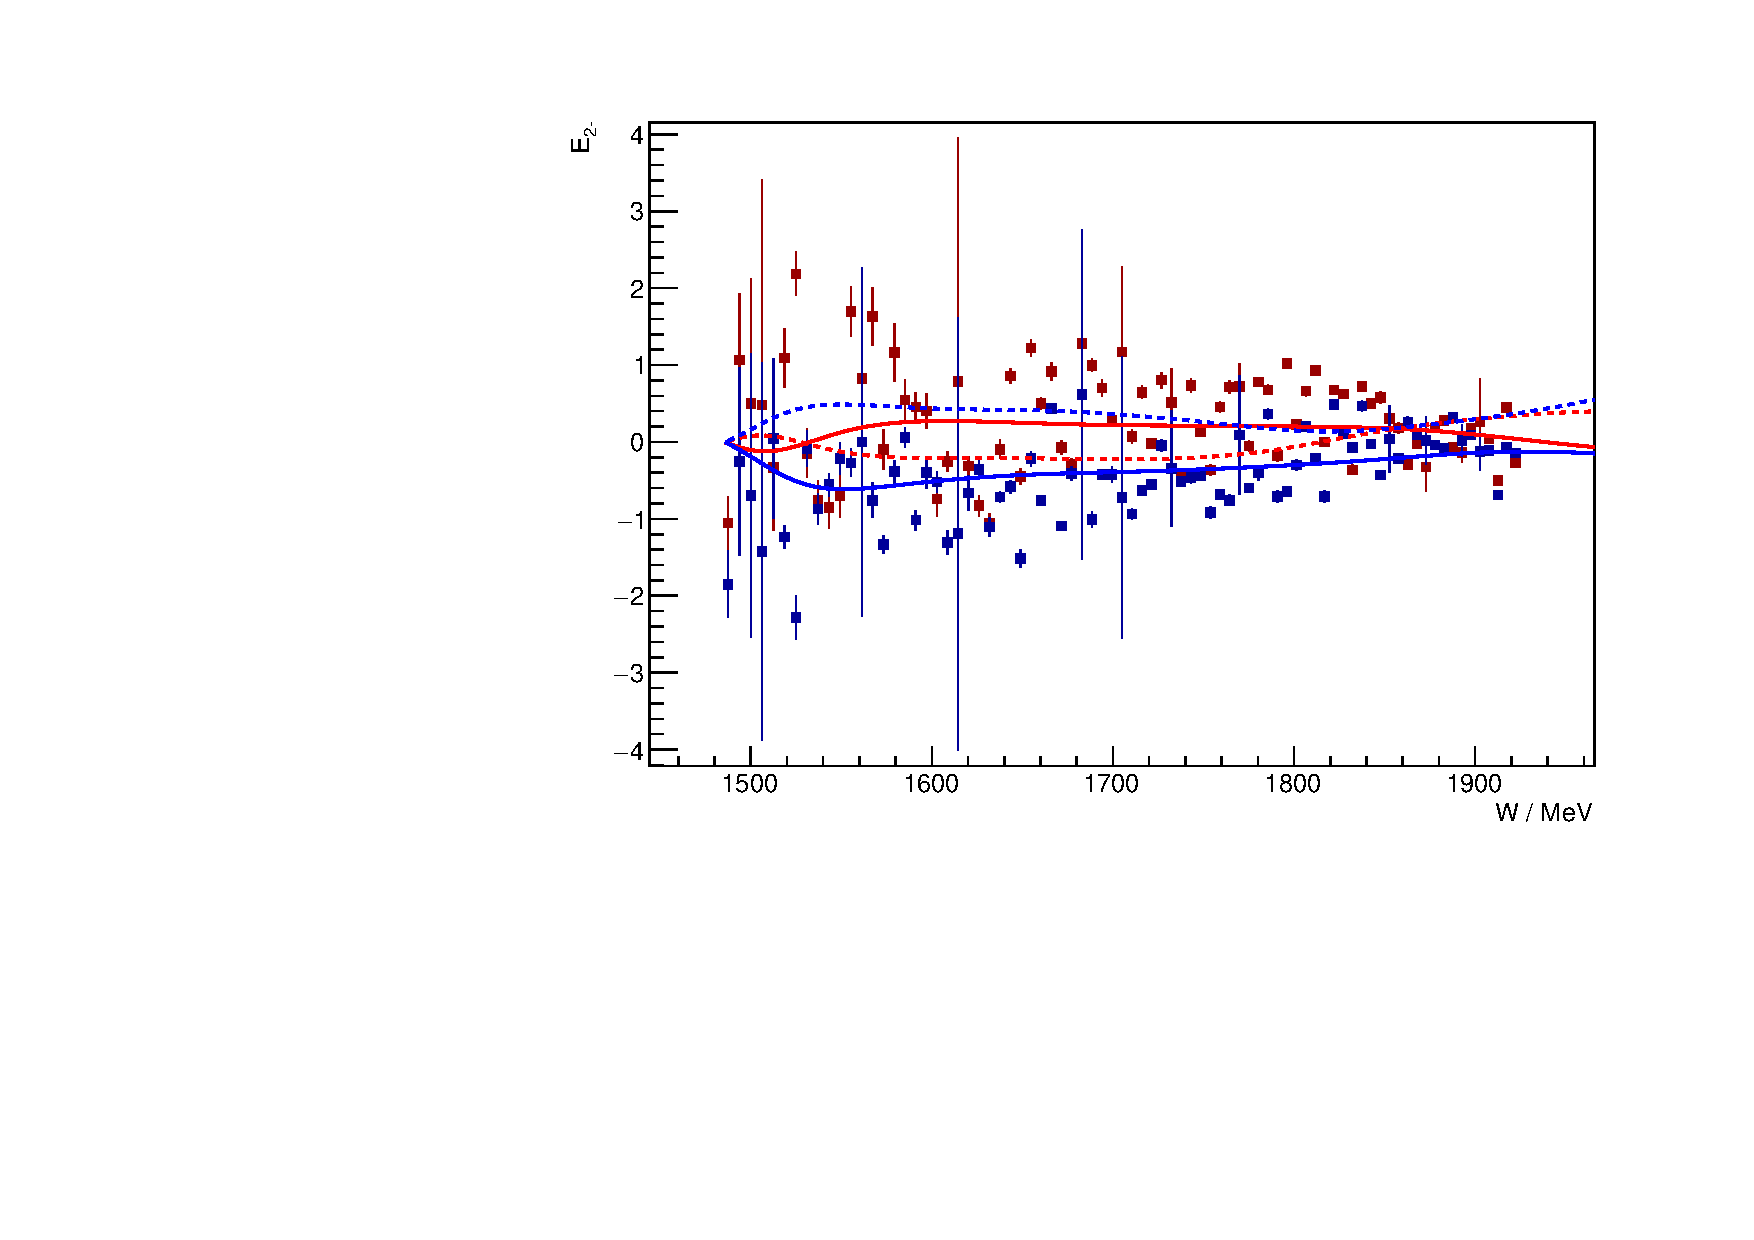
\includegraphics[width=0.49\textwidth]{BnGa/free/plots.0/E2m.pdf}
    }
    \centerline{
    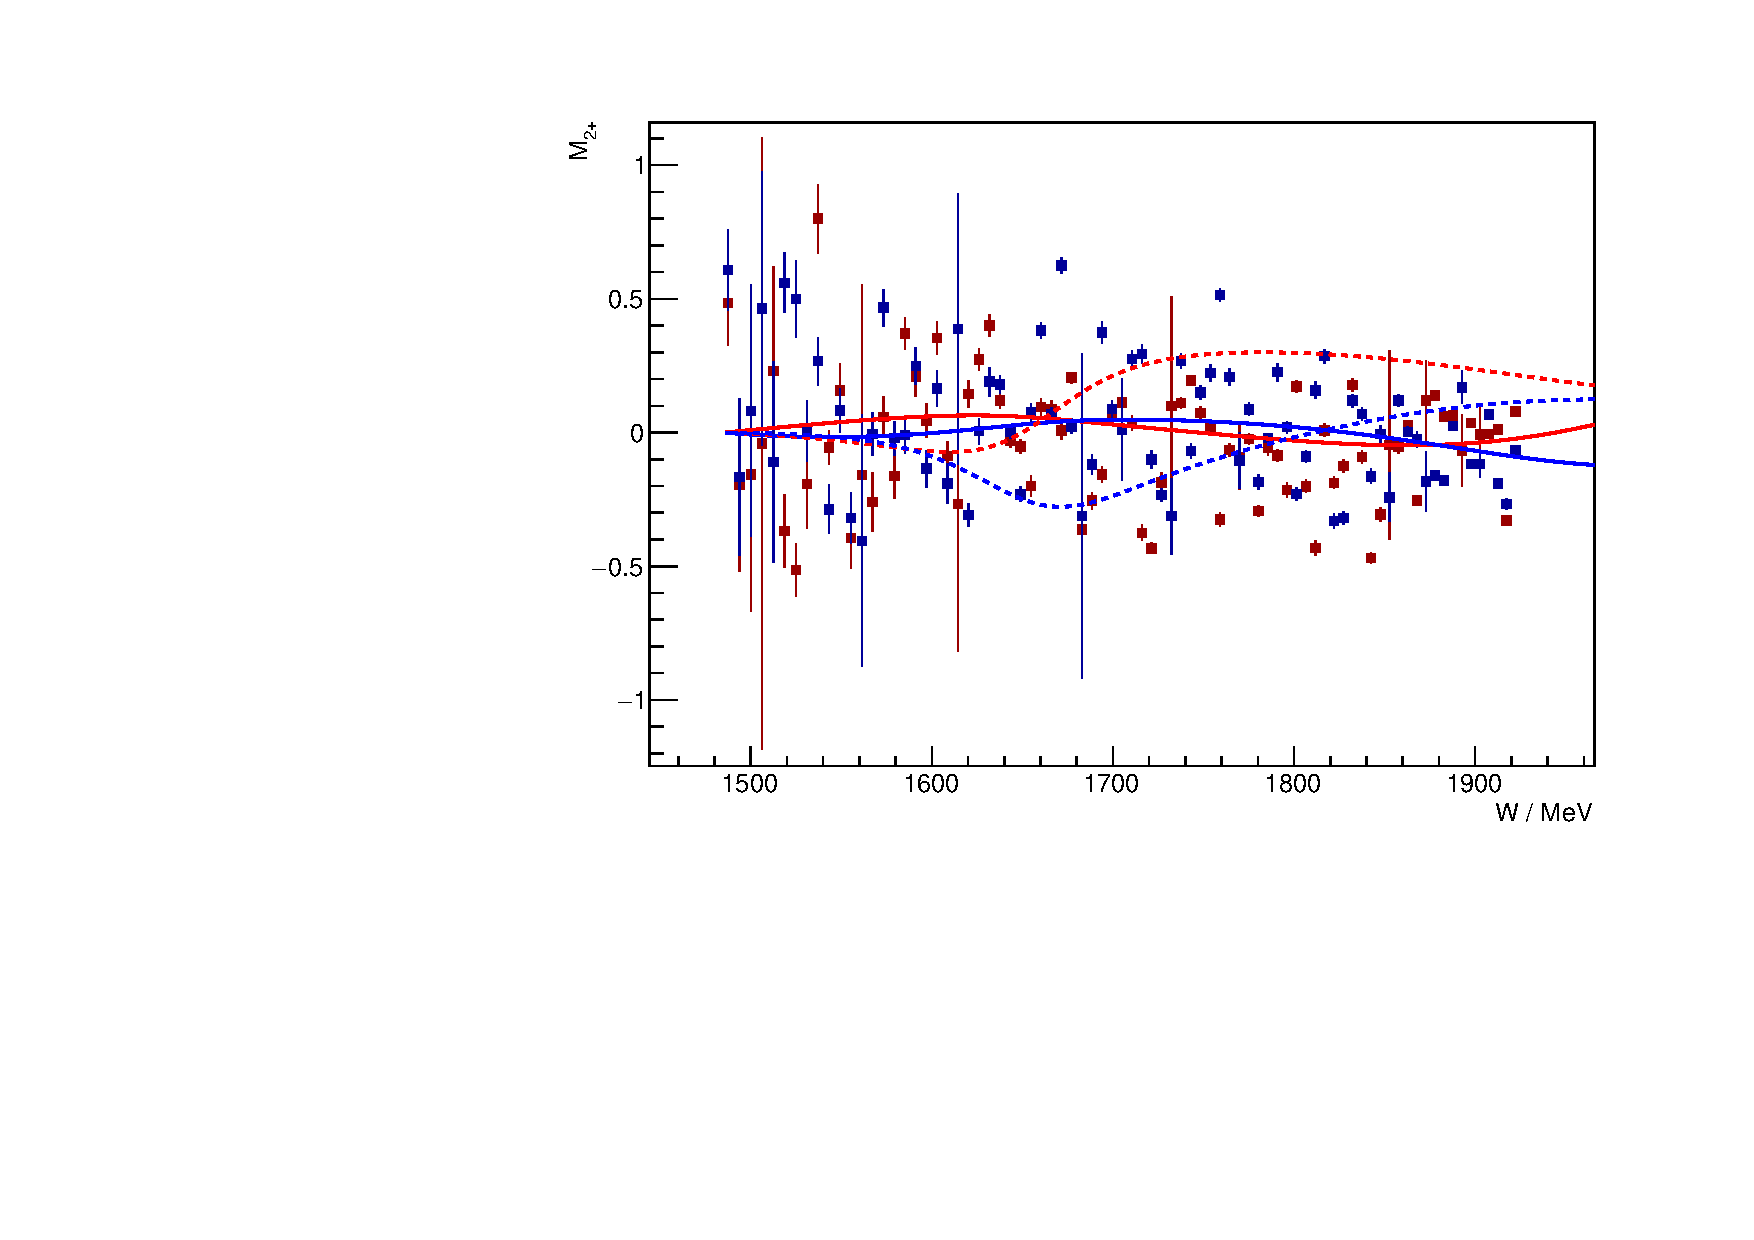
\includegraphics[width=0.49\textwidth]{BnGa/free/plots.0/M2p.pdf}
    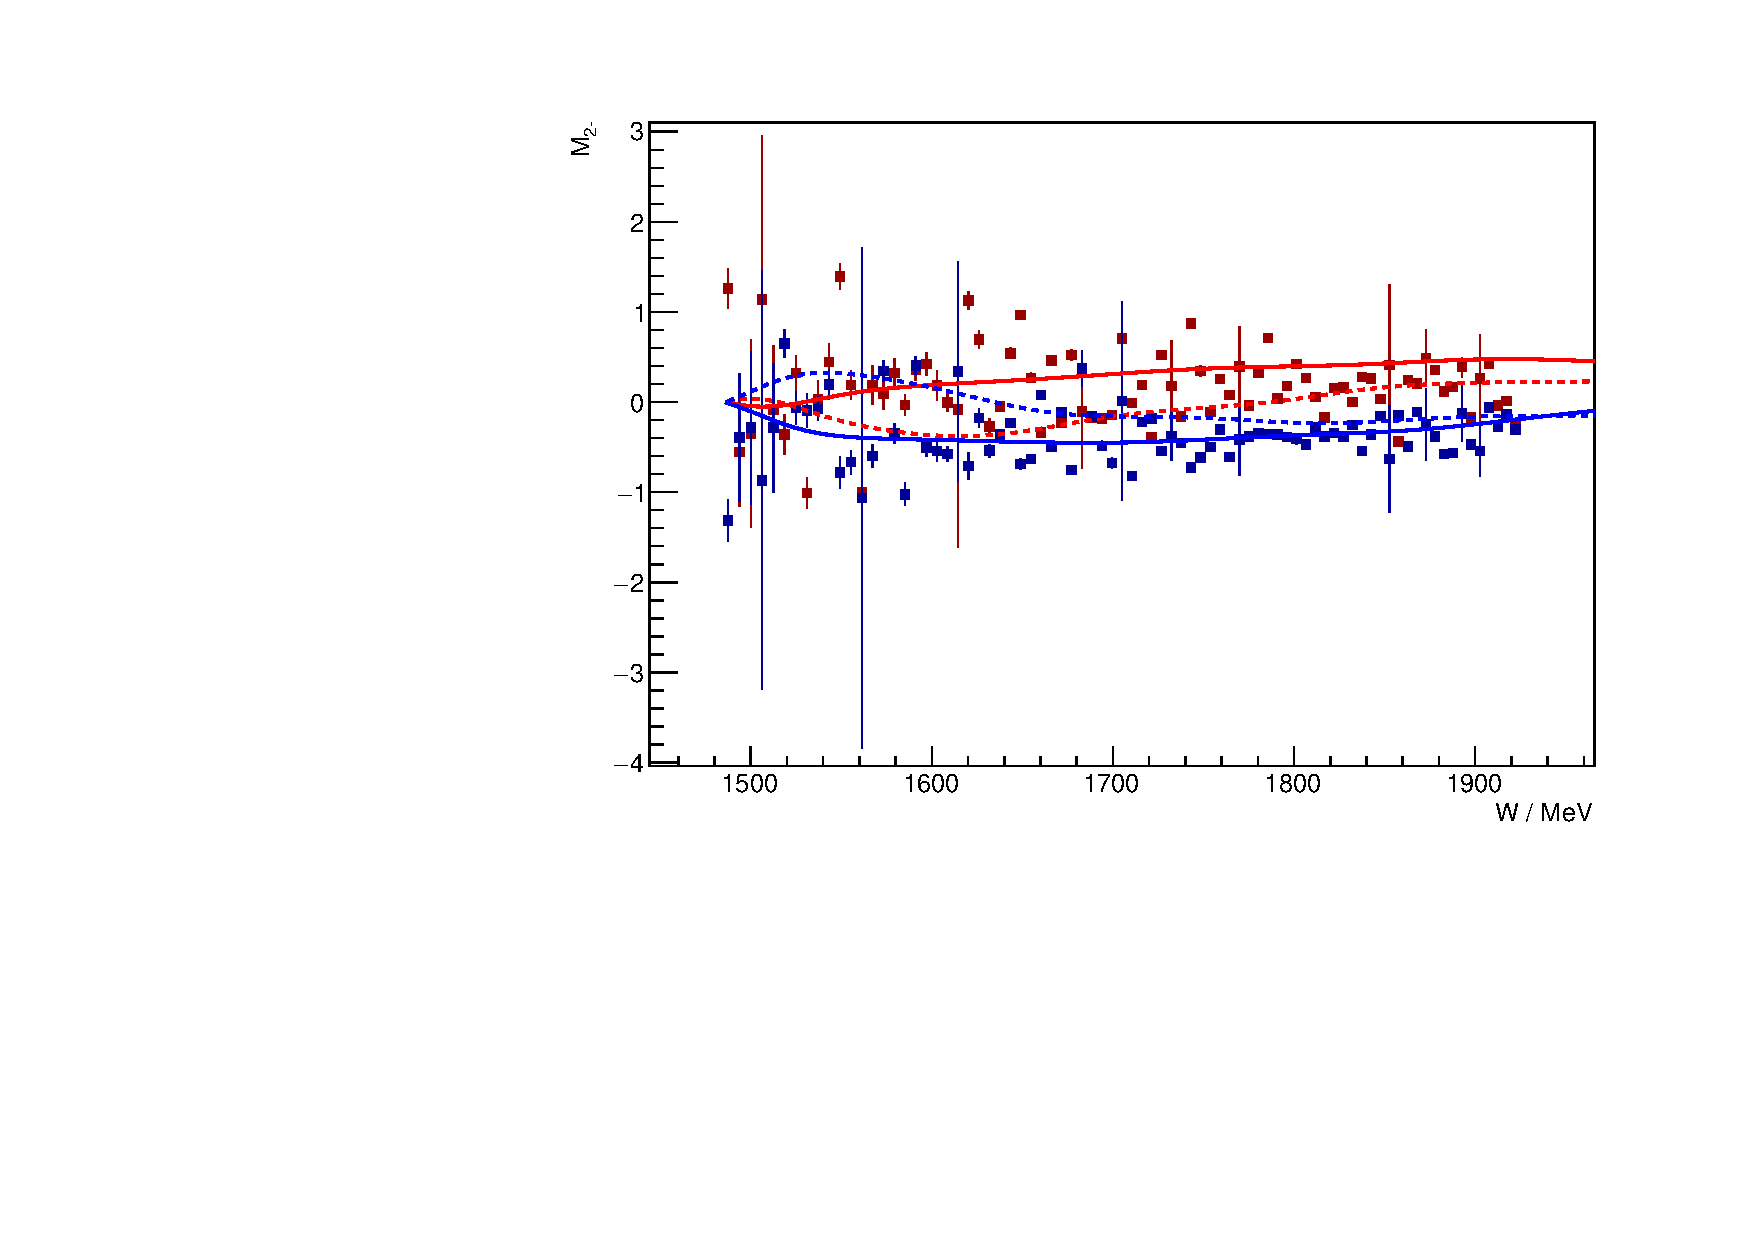
\includegraphics[width=0.49\textwidth]{BnGa/free/plots.0/M2m.pdf}
    }
    \caption{Same as in Fig.~\ref{Fig:free1}. However, the starting parameters of the fit were randomly selected 
    in a 50\% range relative to the BnGa solution (solid lines). The dashed lines show the "true" MAID2015a curves.}
\label{Fig:free2}
  \end{center}
\end{figure}

\begin{figure}
  \begin{center}
    \centerline{
    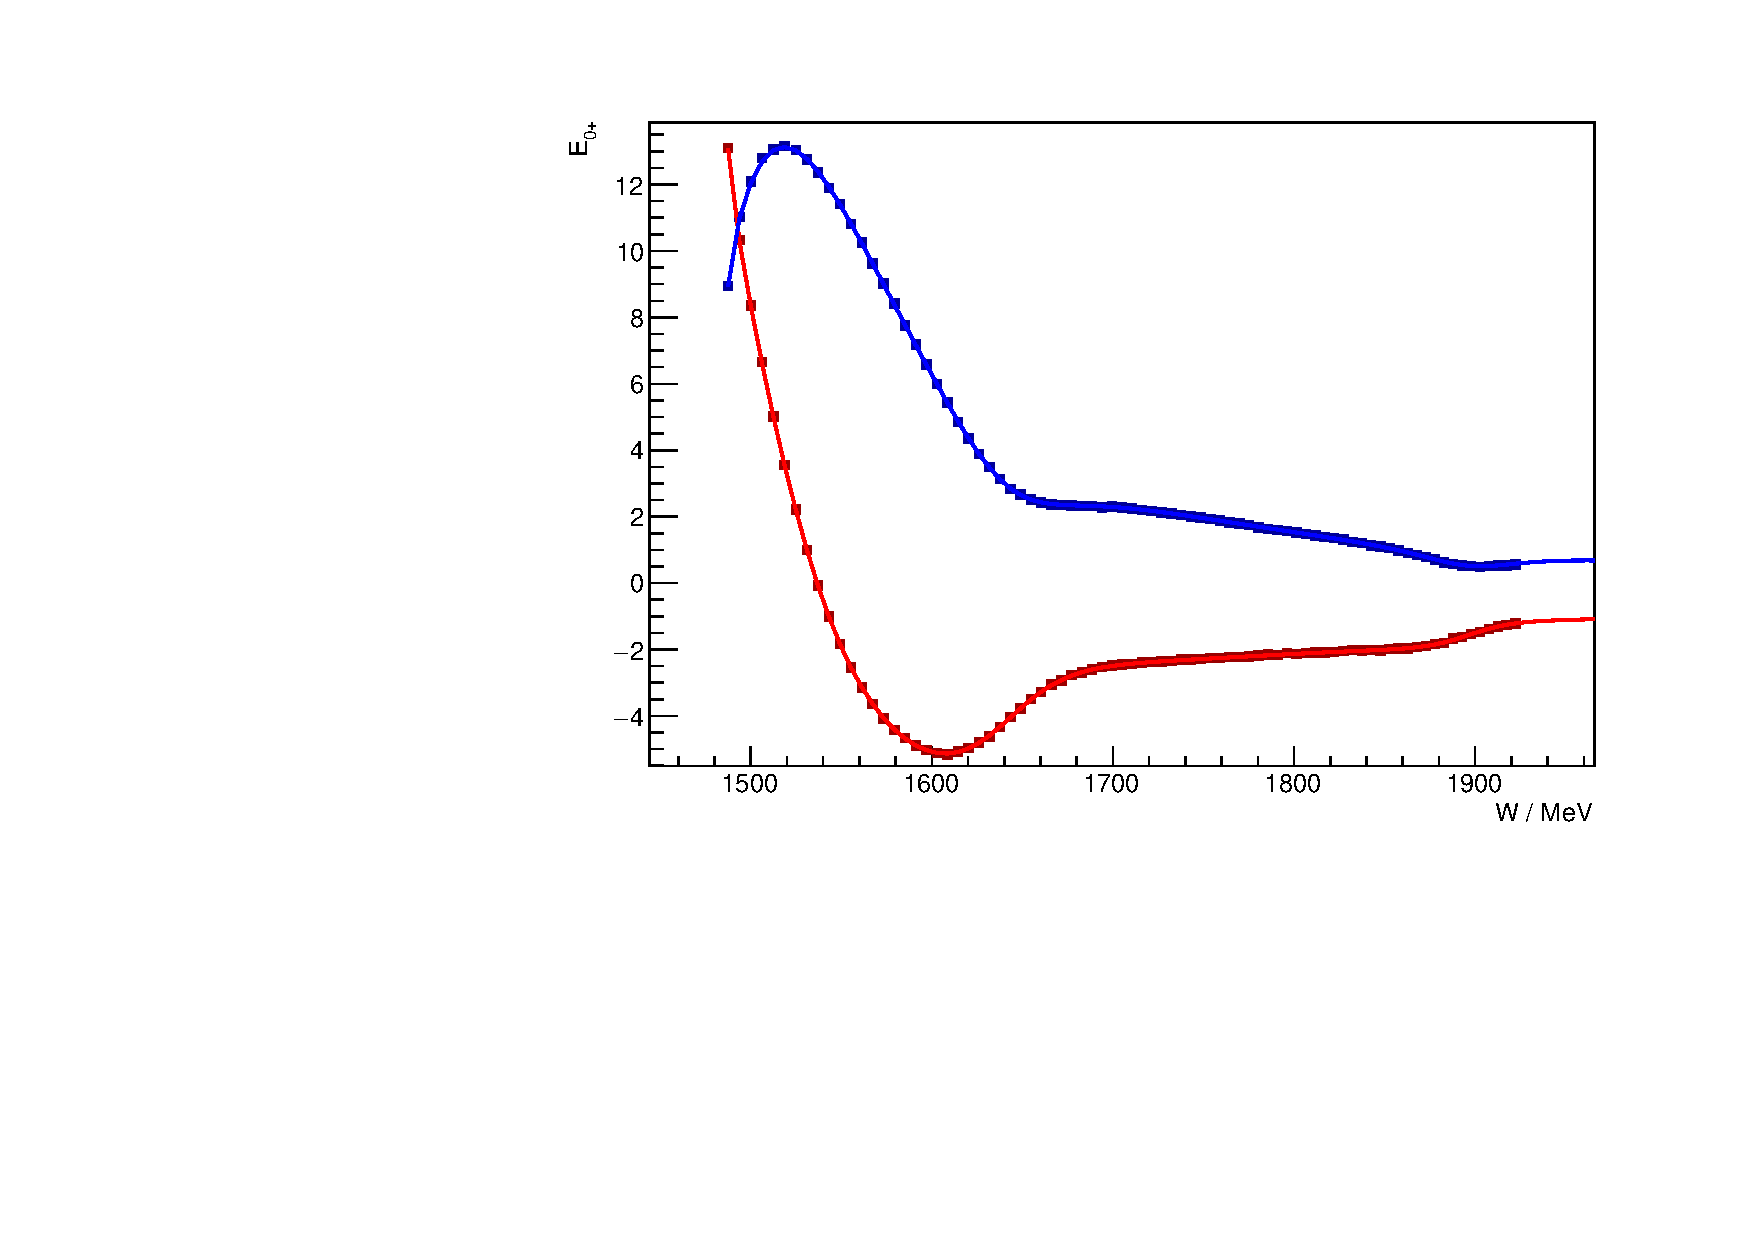
\includegraphics[width=0.49\textwidth]{MAID2015a/PenHeli_dat/plots.0/E0p.pdf}
    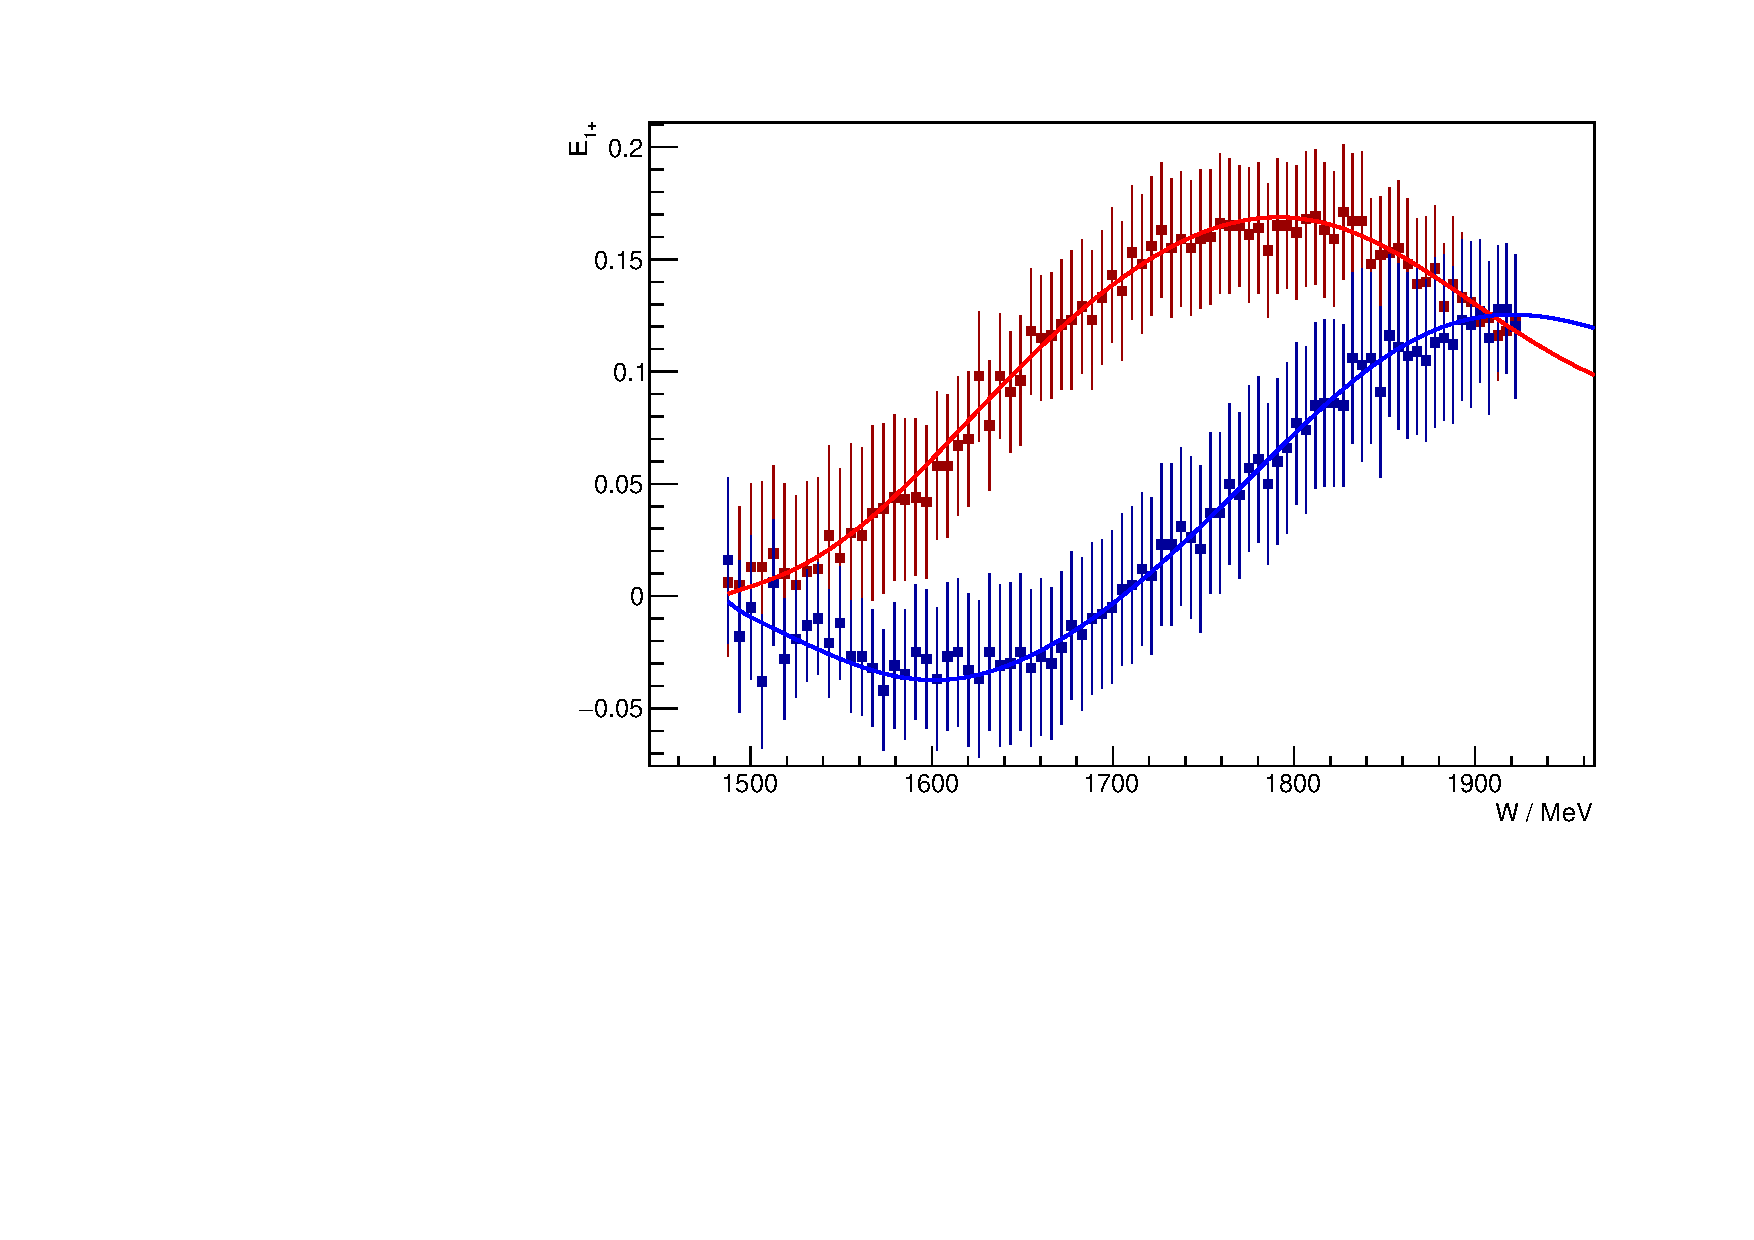
\includegraphics[width=0.49\textwidth]{MAID2015a/PenHeli_dat/plots.0/E1p.pdf}
    }
    \centerline{
    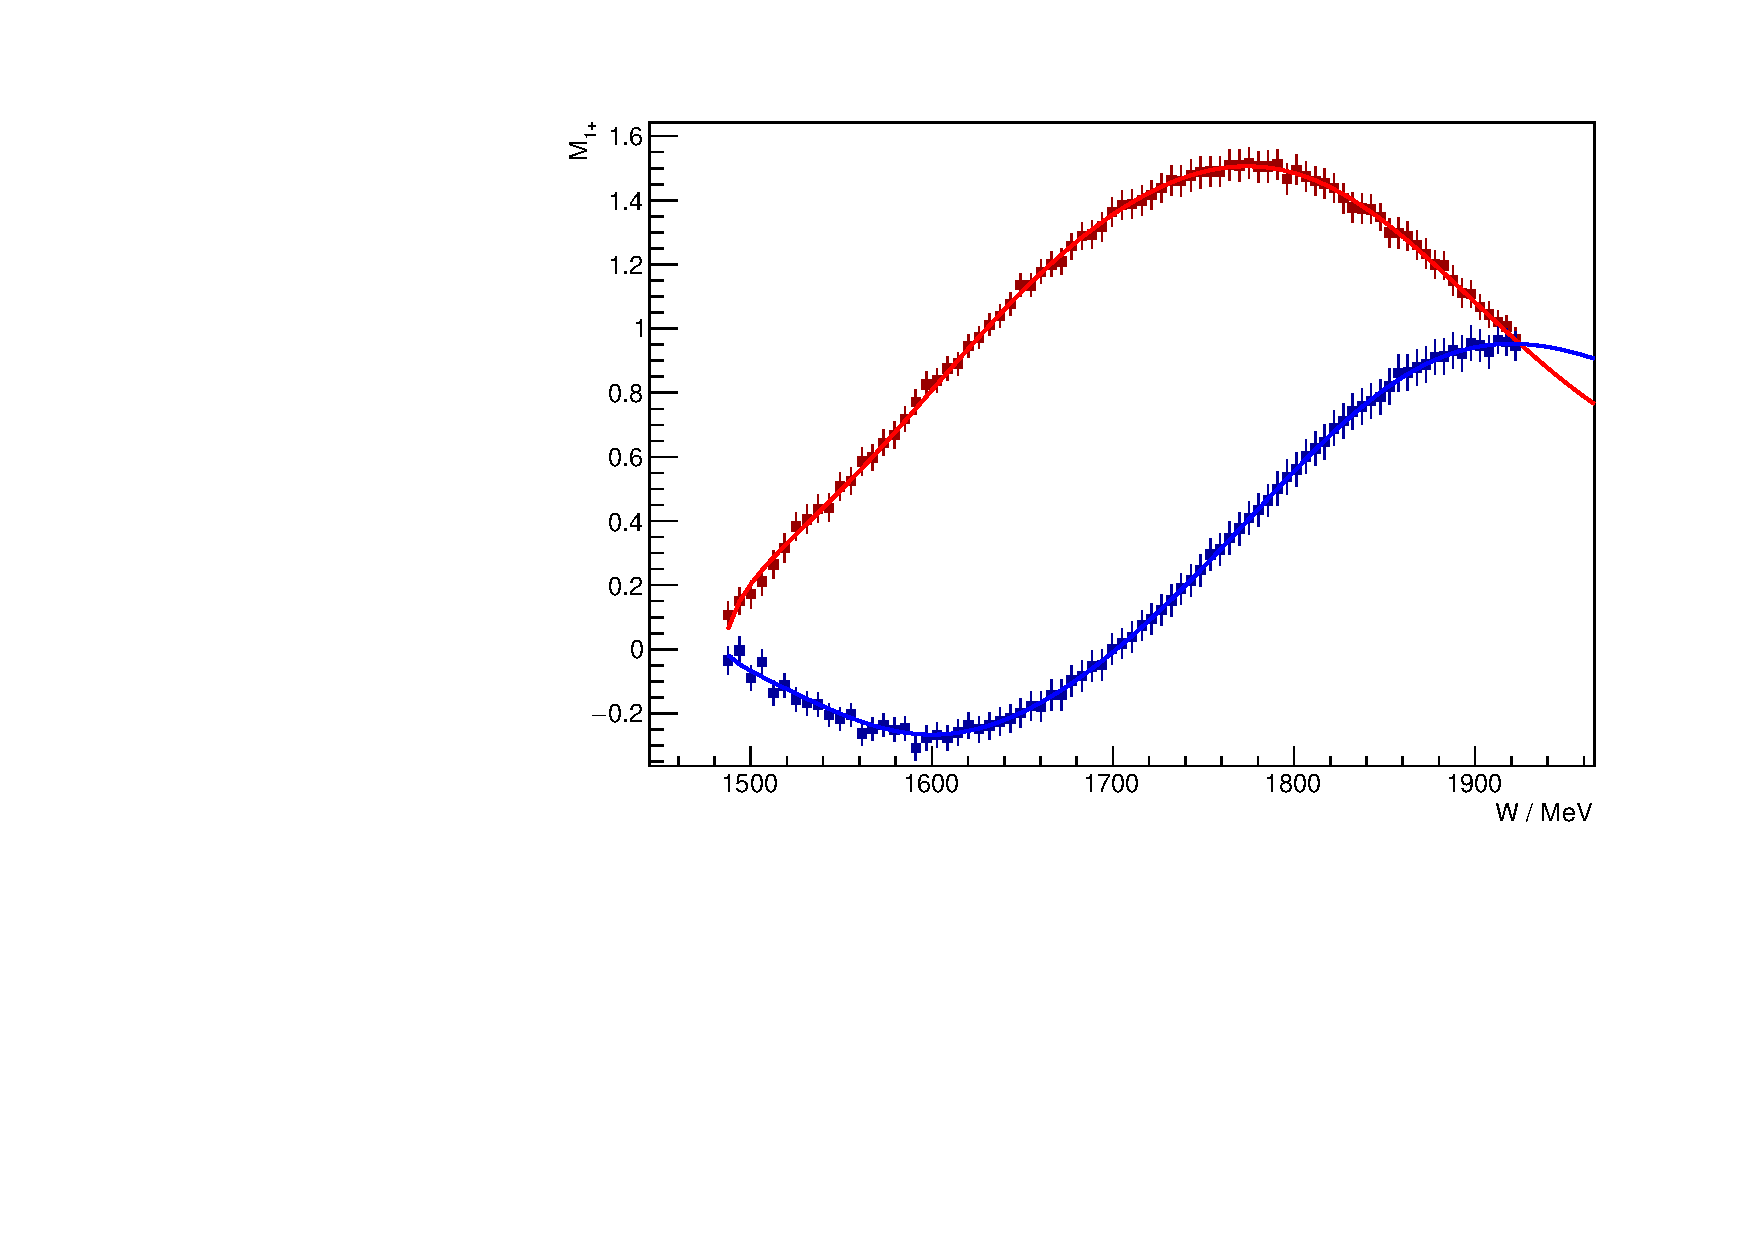
\includegraphics[width=0.49\textwidth]{MAID2015a/PenHeli_dat/plots.0/M1p.pdf}
    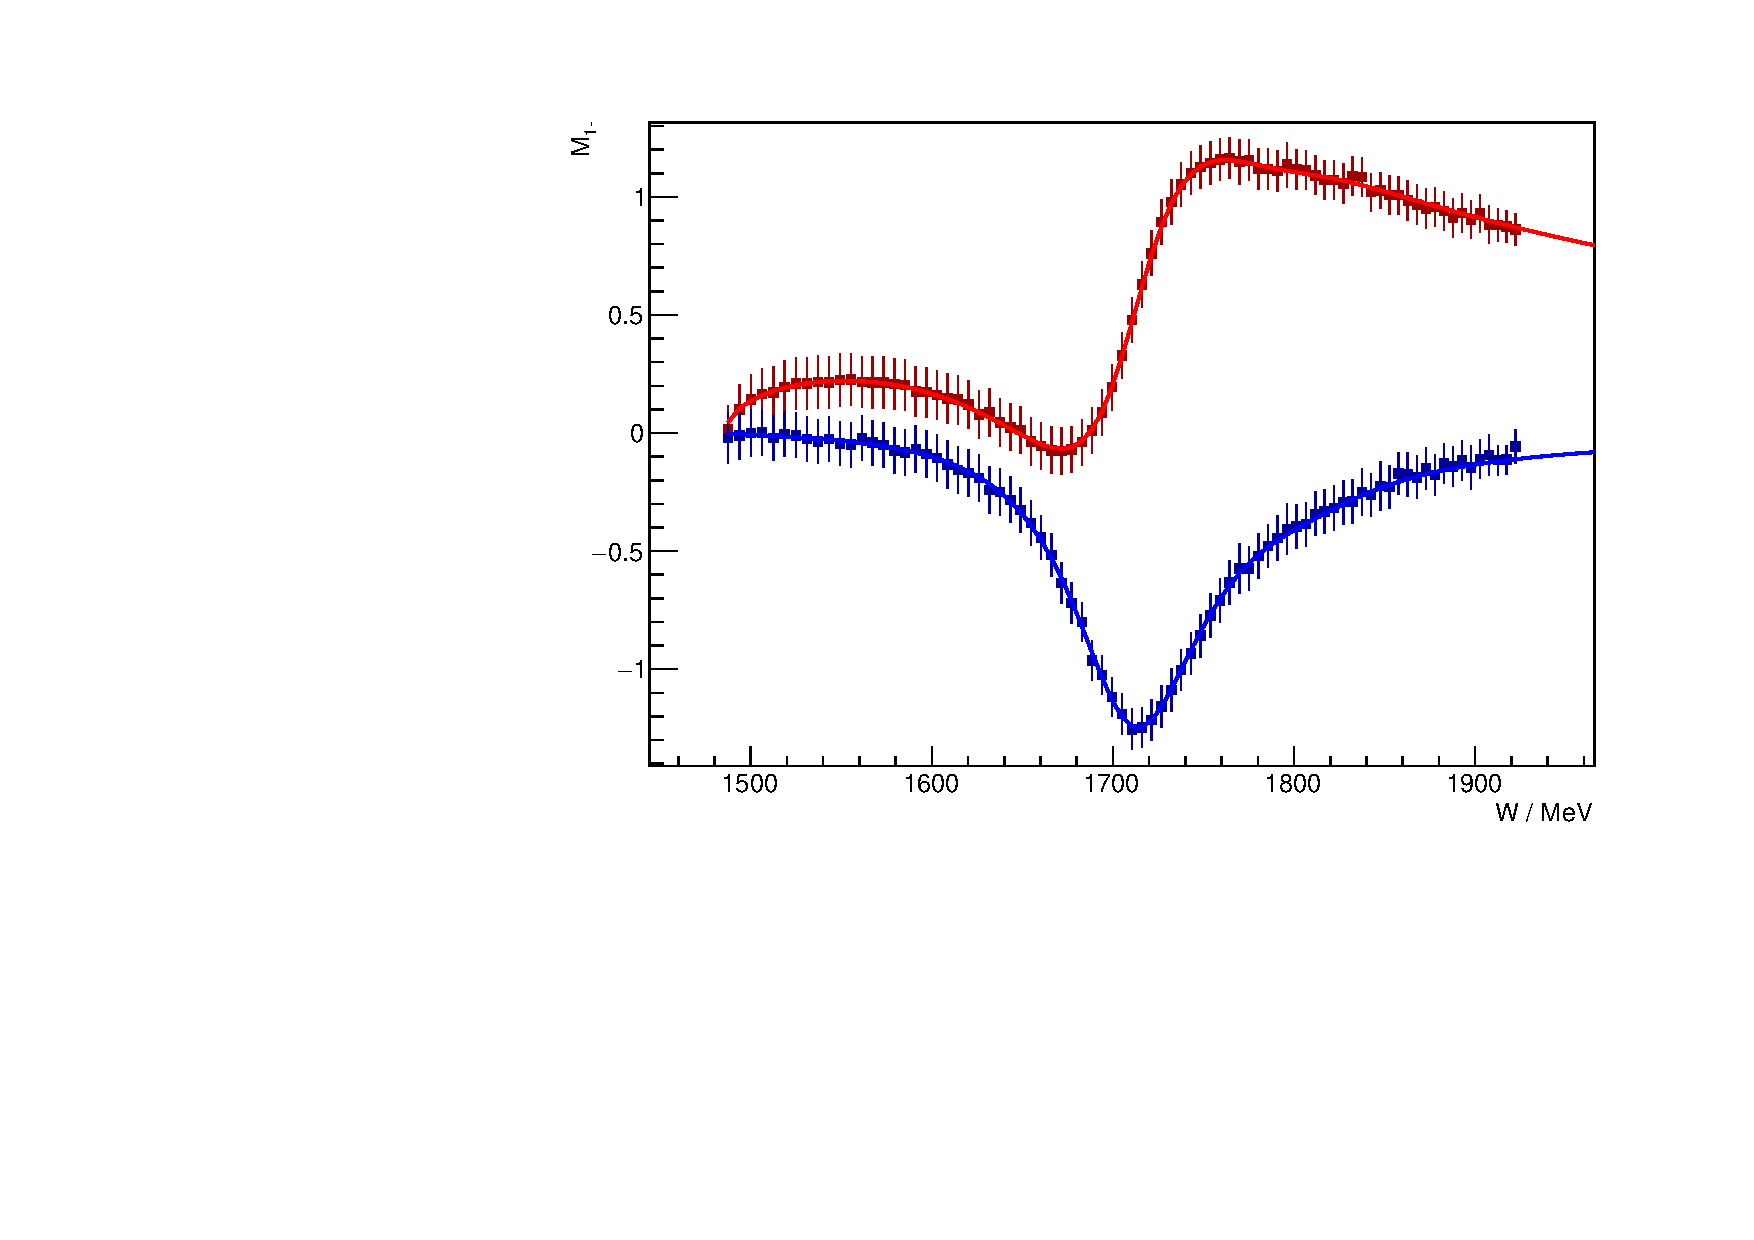
\includegraphics[width=0.49\textwidth]{MAID2015a/PenHeli_dat/plots.0/M1m.pdf}
    }
    \centerline{
    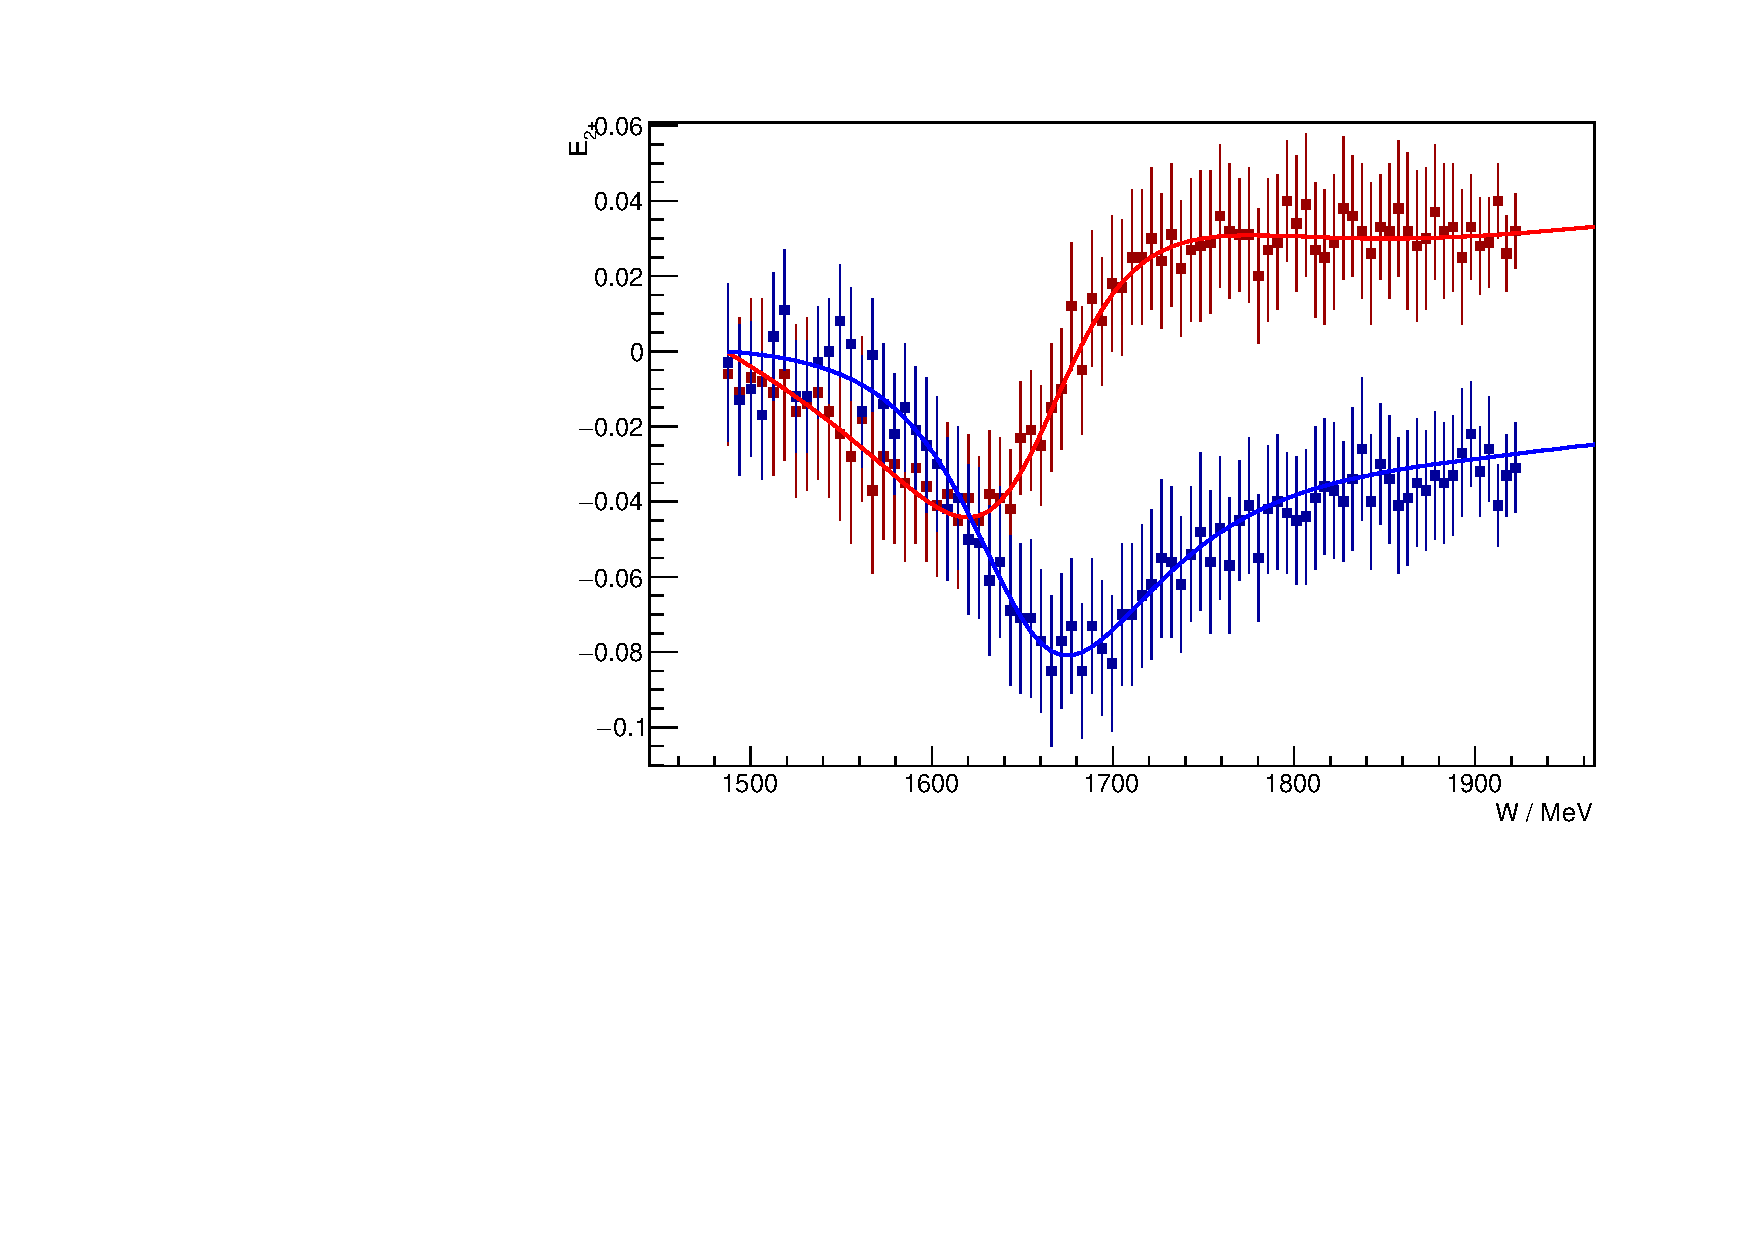
\includegraphics[width=0.49\textwidth]{MAID2015a/PenHeli_dat/plots.0/E2p.pdf}
    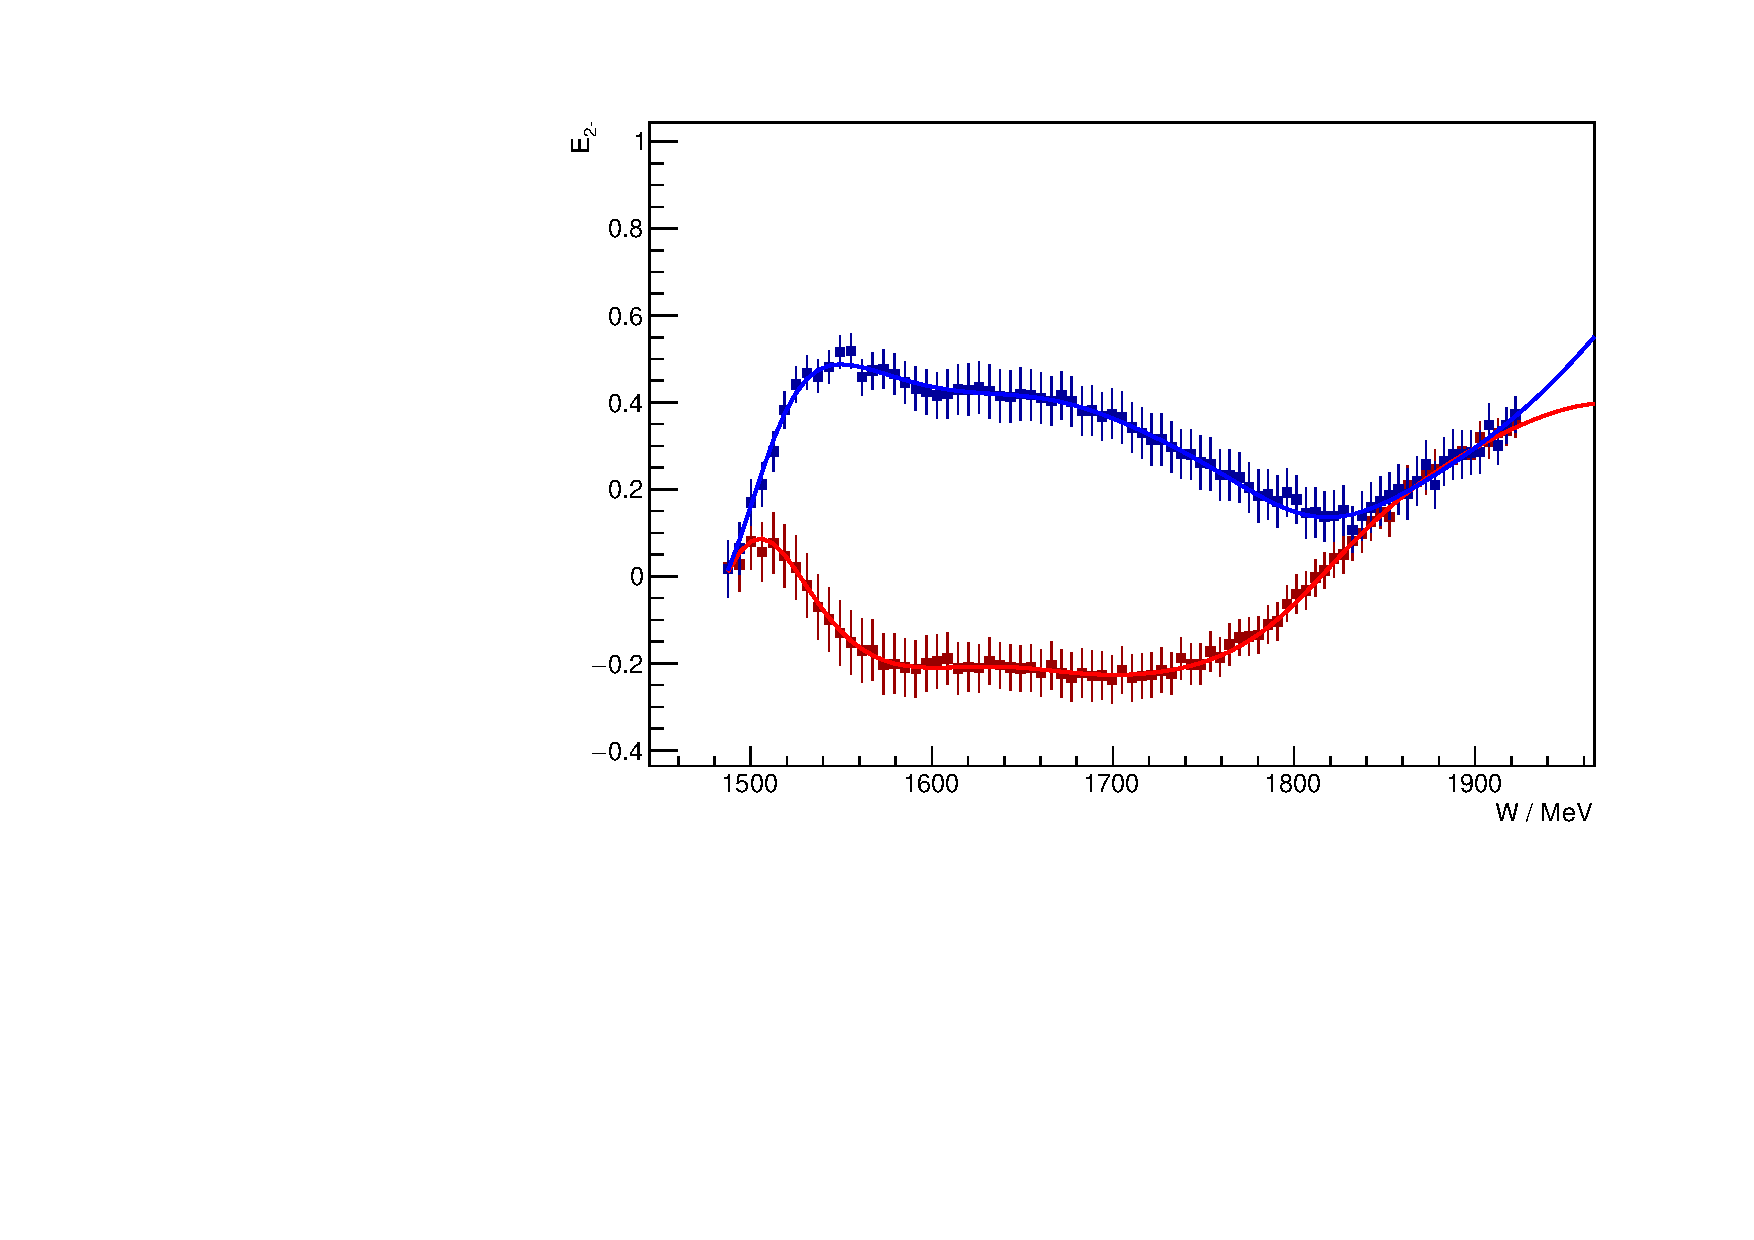
\includegraphics[width=0.49\textwidth]{MAID2015a/PenHeli_dat/plots.0/E2m.pdf}
    }
    \centerline{
    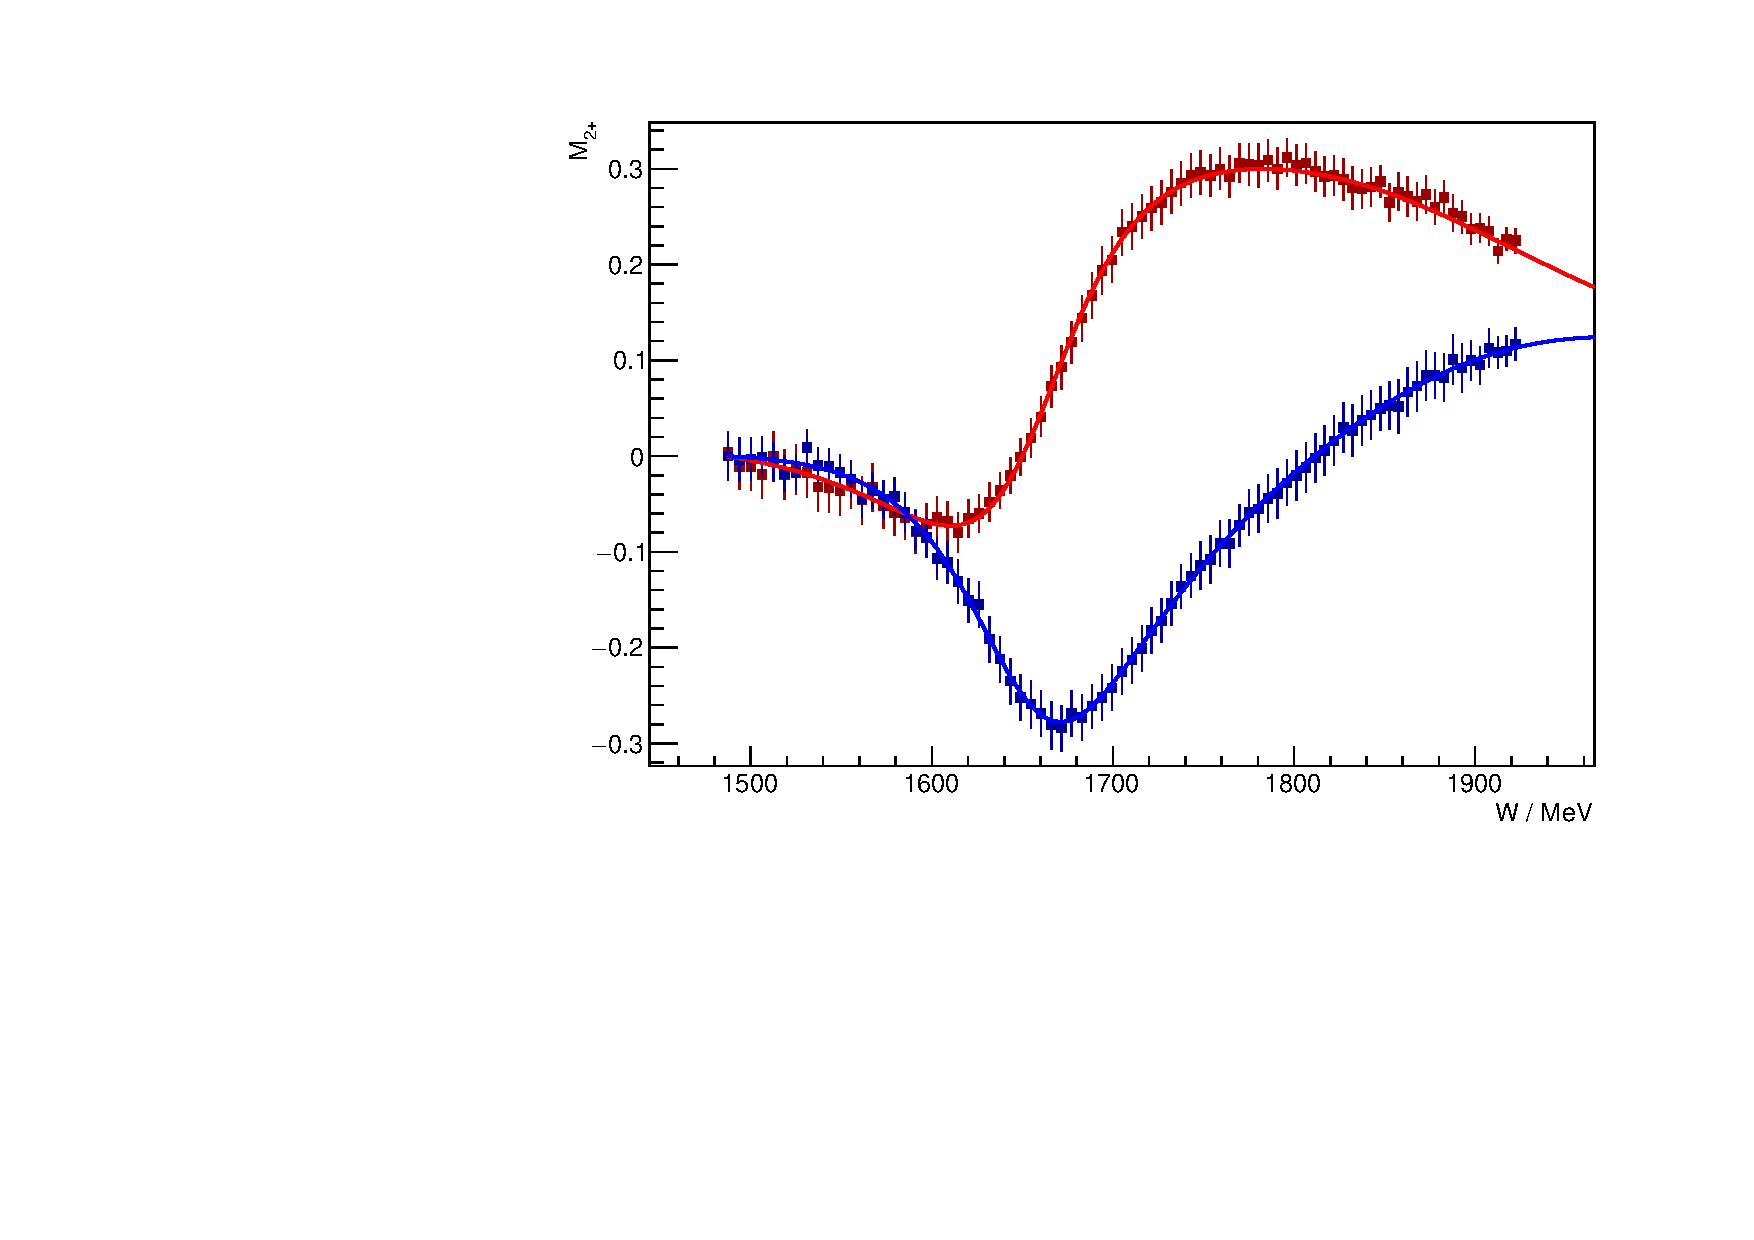
\includegraphics[width=0.49\textwidth]{MAID2015a/PenHeli_dat/plots.0/M2p.pdf}
    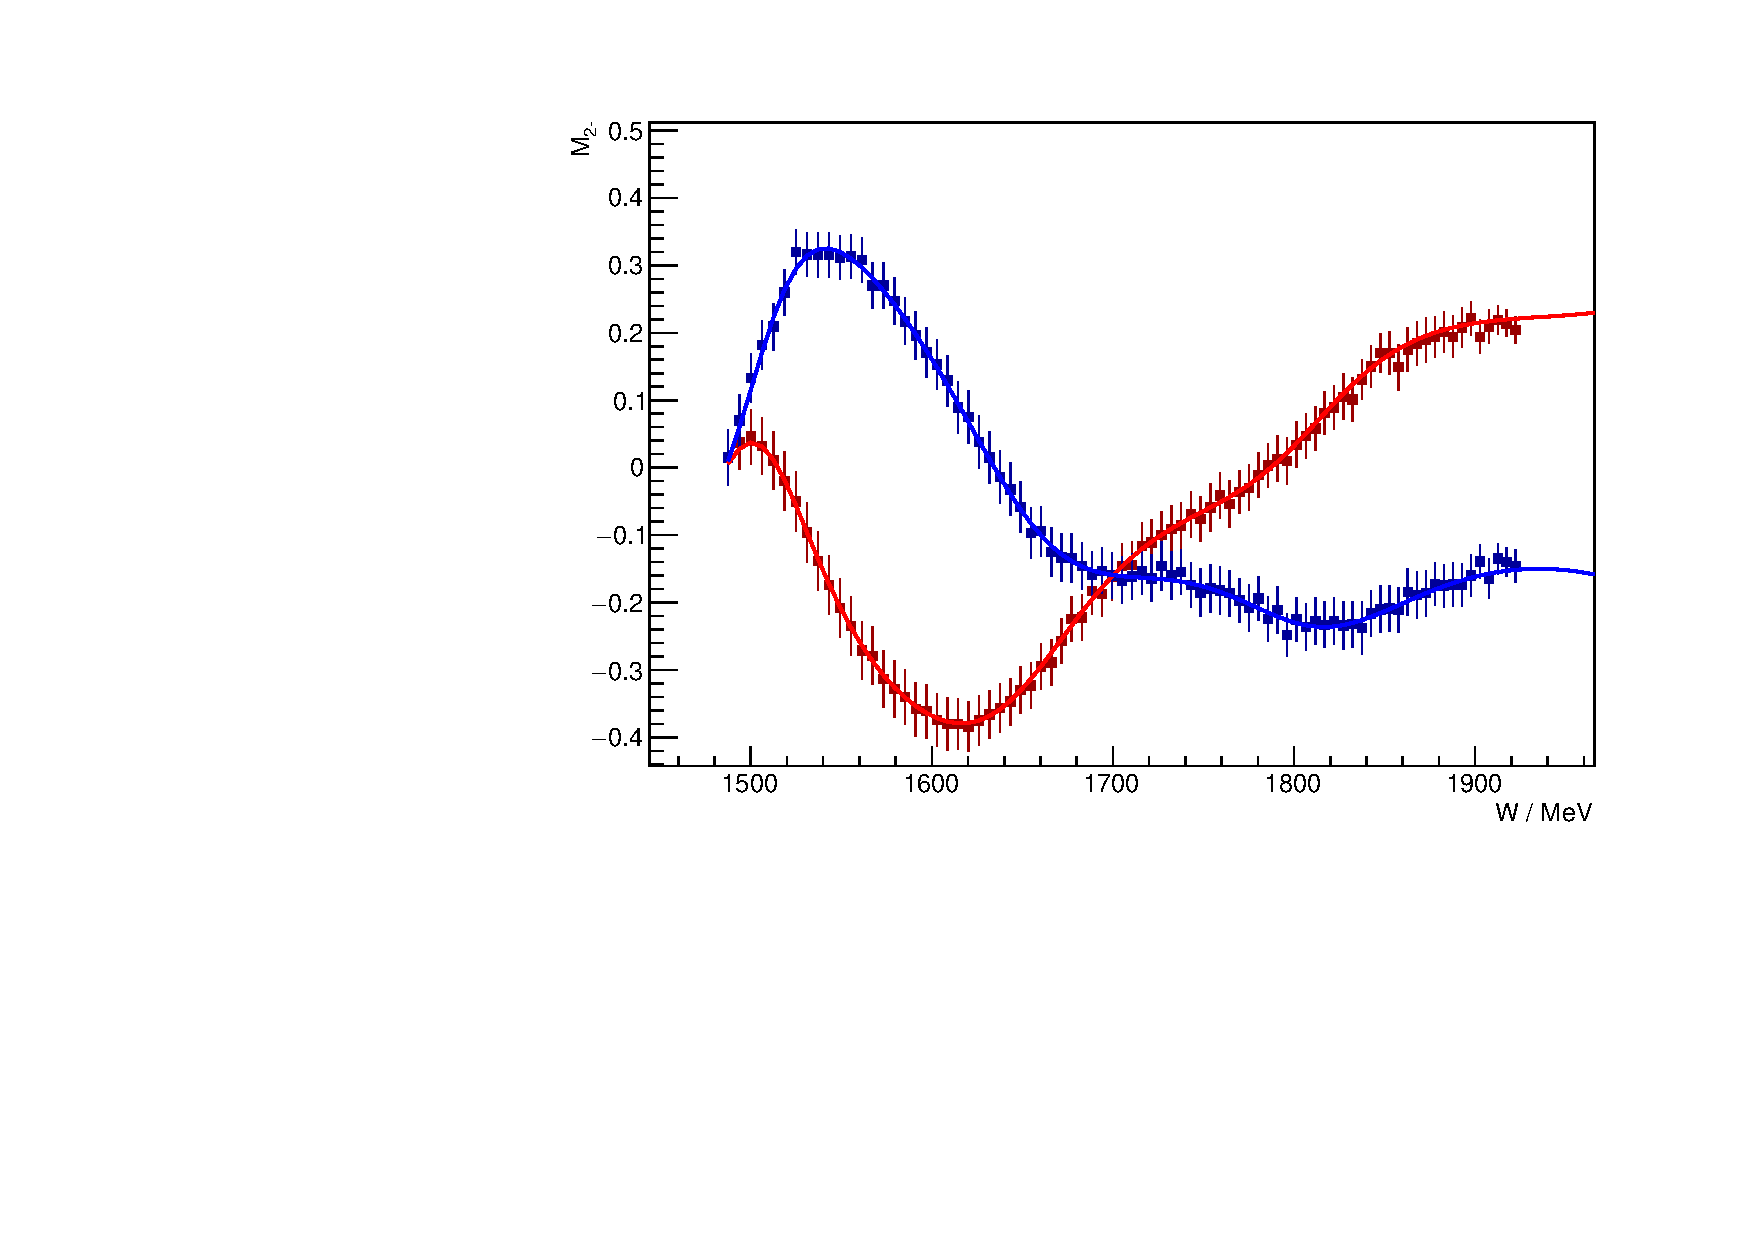
\includegraphics[width=0.49\textwidth]{MAID2015a/PenHeli_dat/plots.0/M2m.pdf}
    }
    \caption{s-, p- and d-wave multipoles from a fit constrained to the "true" MAID2015a helicity amplitudes. 
    Starting values: 50\% range around the MAID15a solution.}
\label{Fig:const1}
  \end{center}
\end{figure}

\begin{figure}
  \begin{center}
    \centerline{
    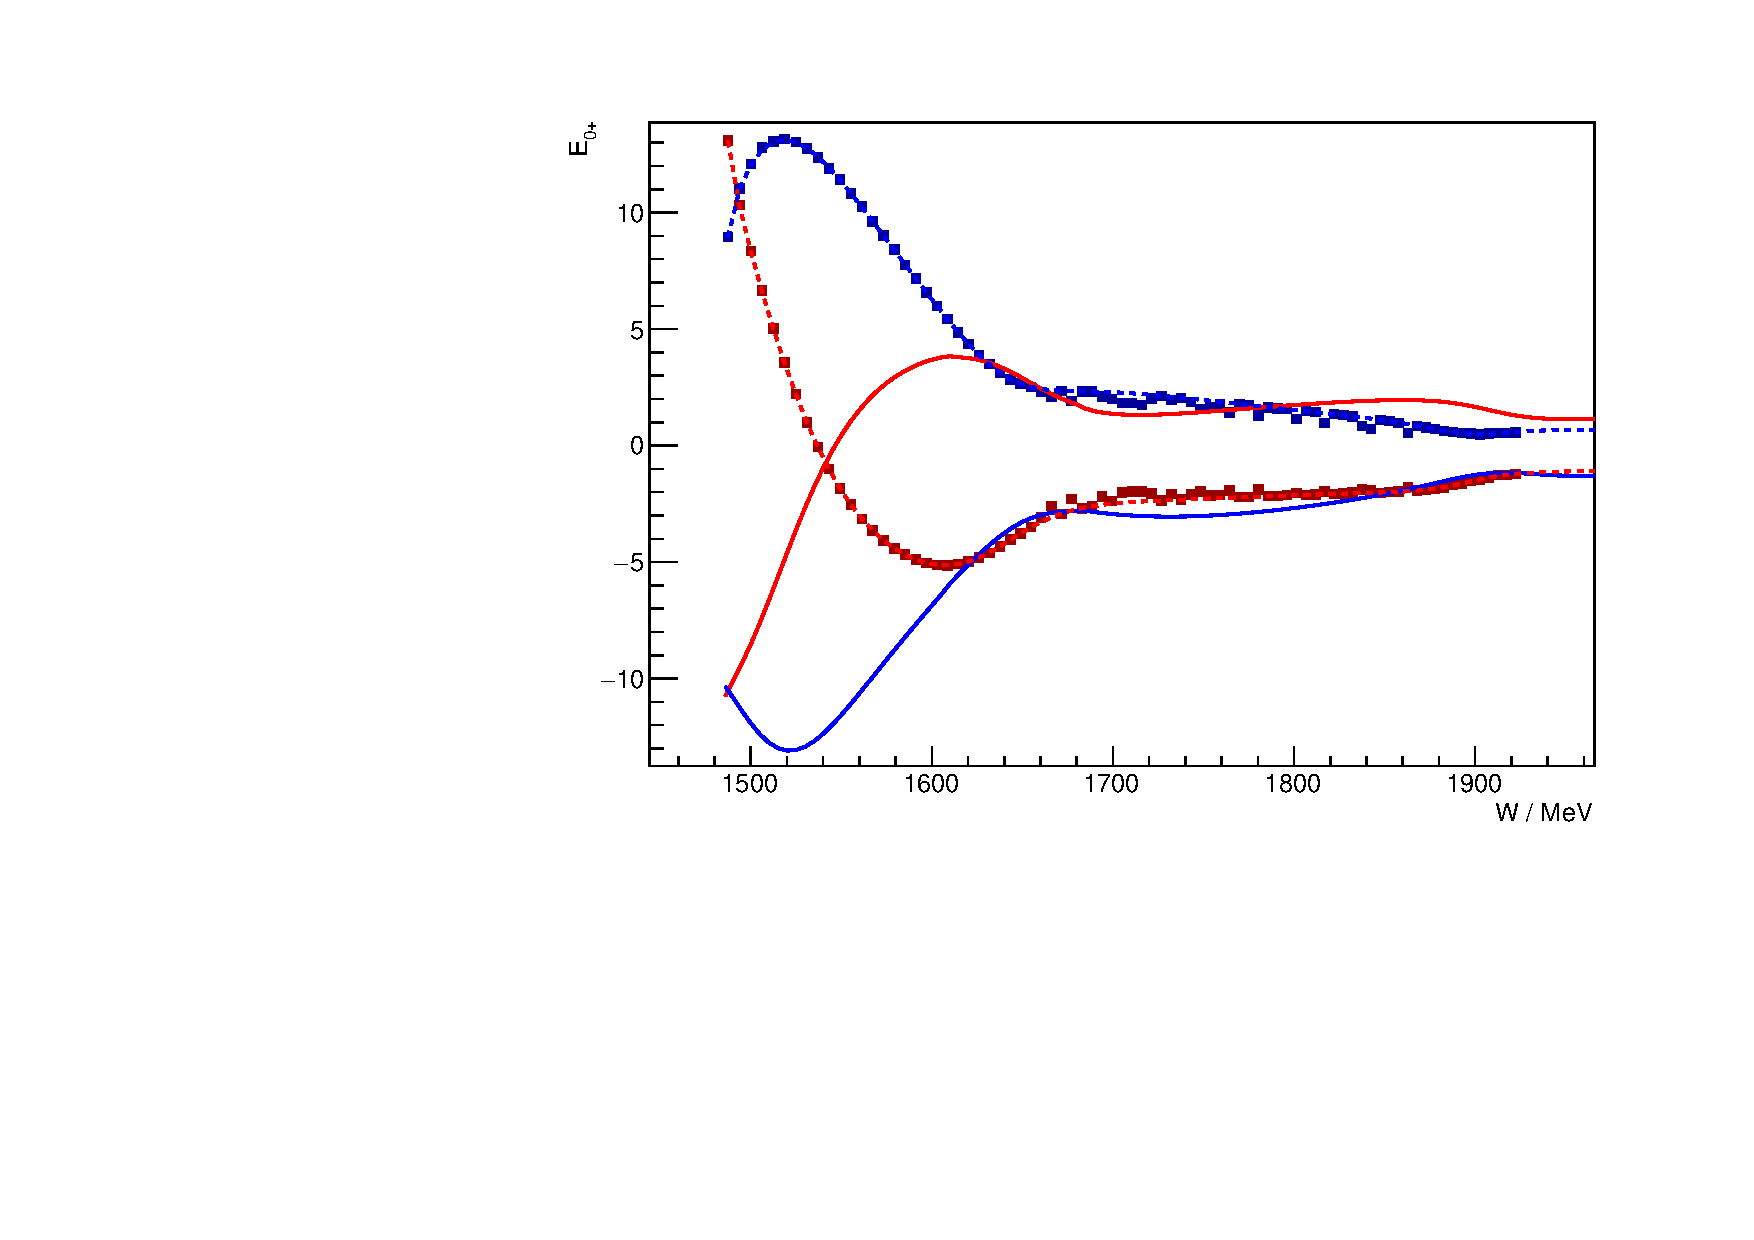
\includegraphics[width=0.49\textwidth]{BnGa/PenHeli/plots.0/E0p.pdf}
    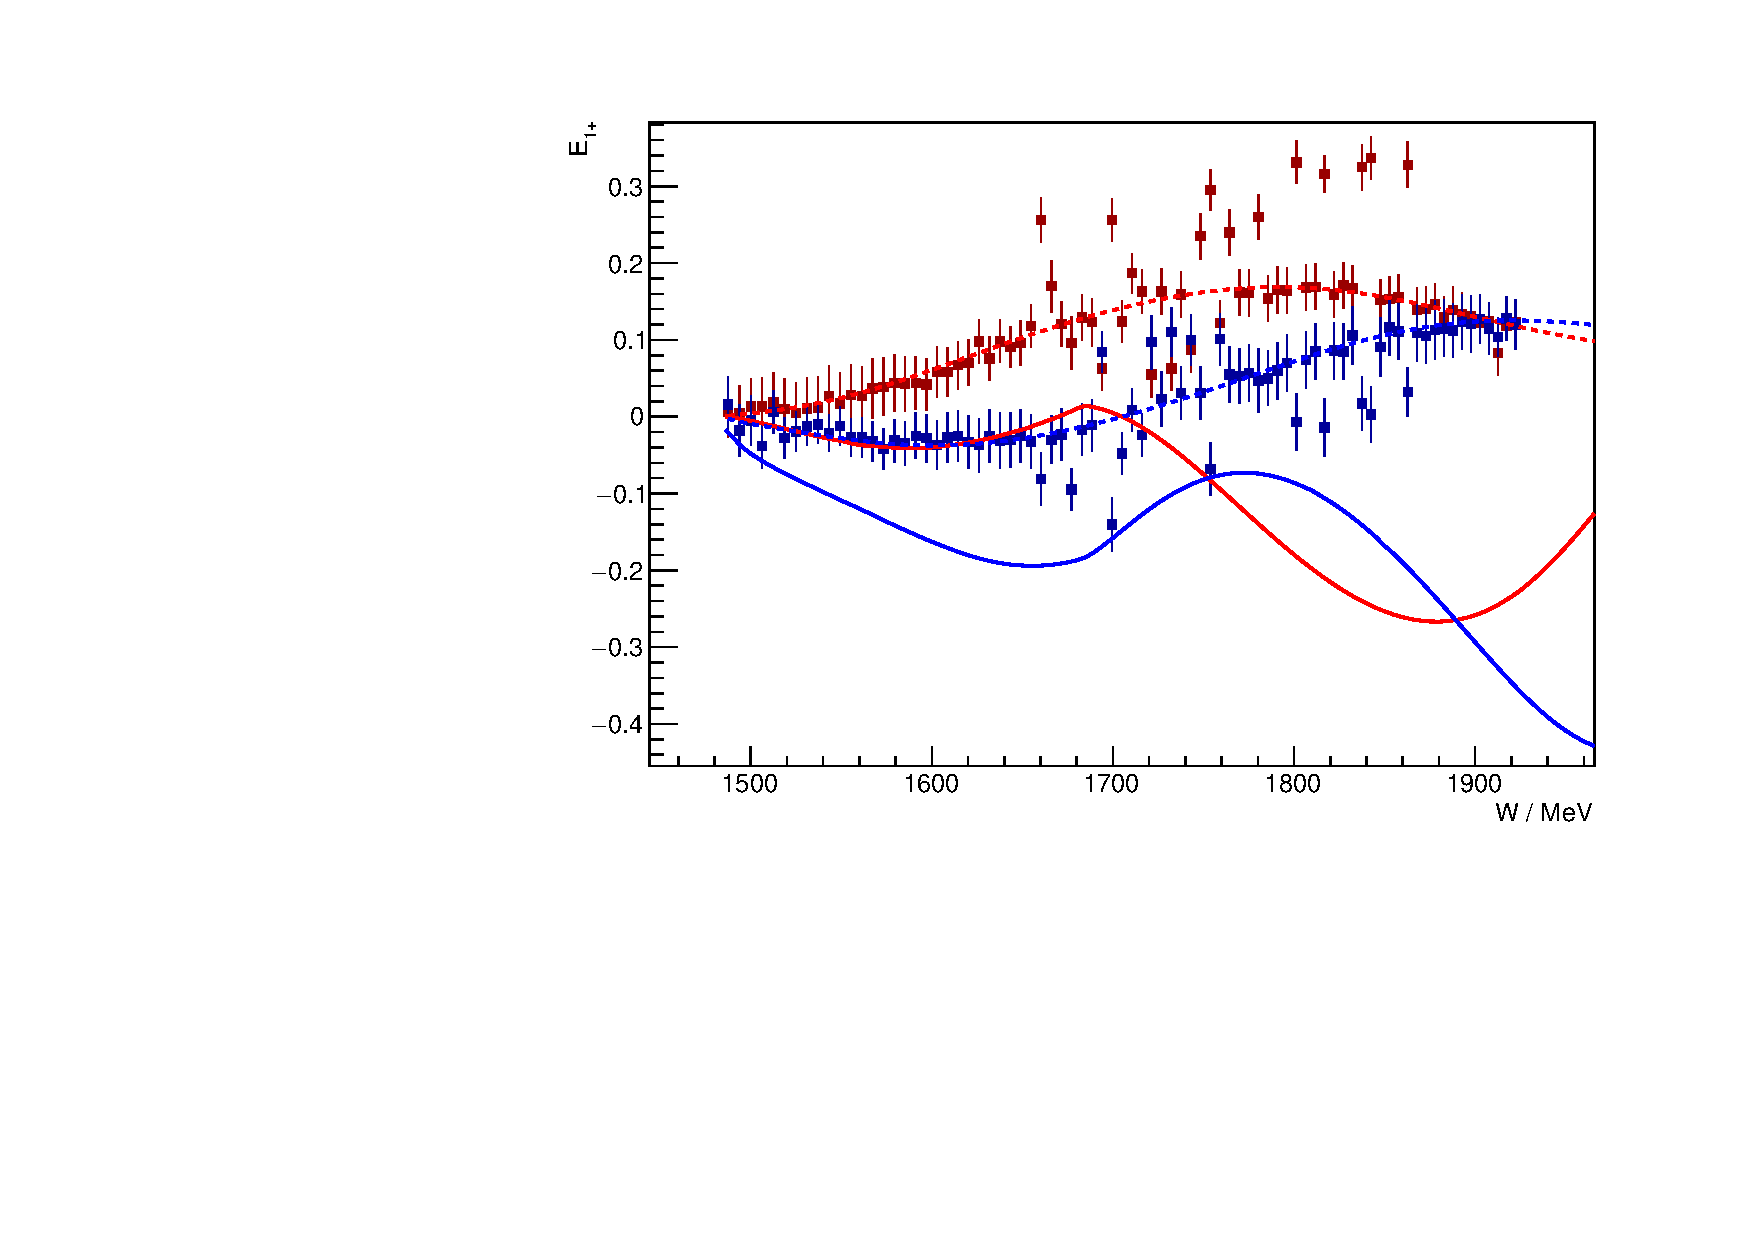
\includegraphics[width=0.49\textwidth]{BnGa/PenHeli/plots.0/E1p.pdf}
    }
    \centerline{
    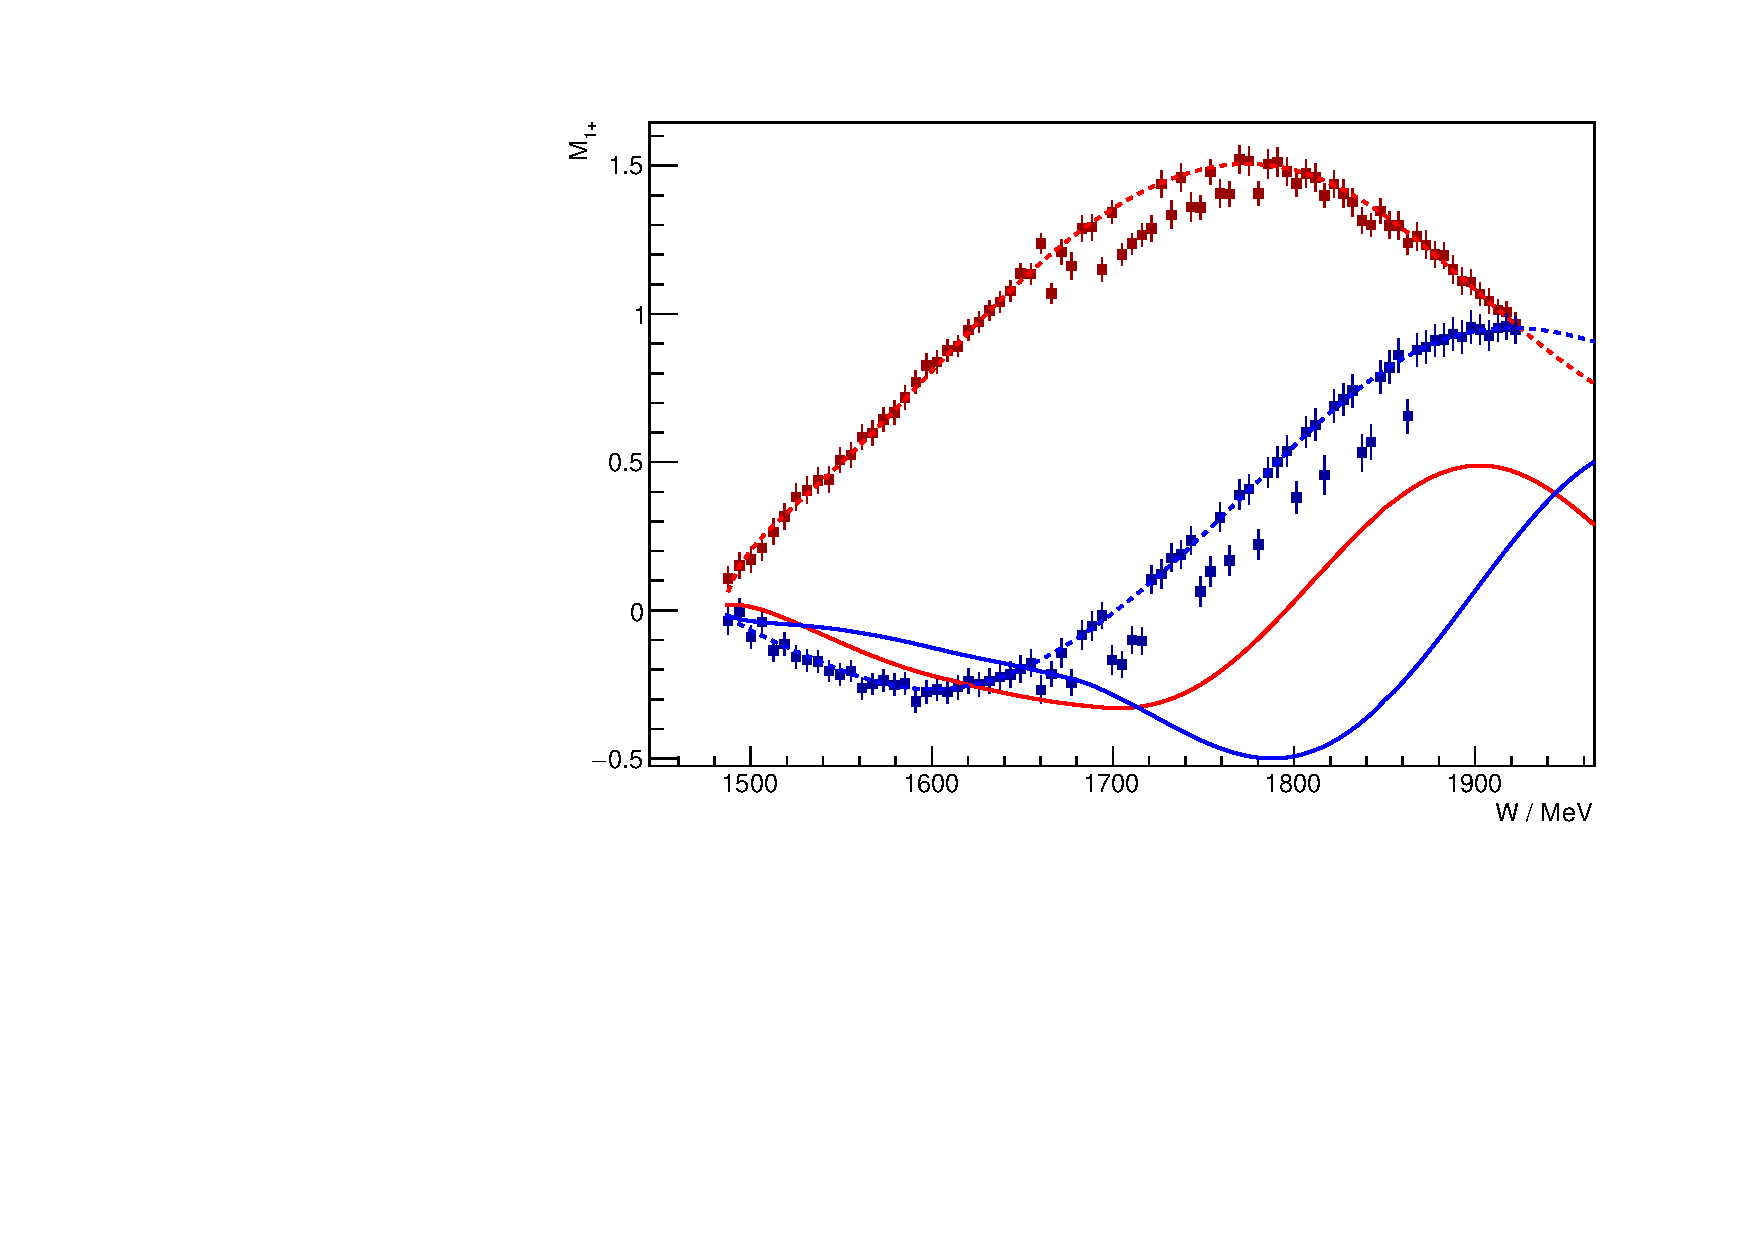
\includegraphics[width=0.49\textwidth]{BnGa/PenHeli/plots.0/M1p.pdf}
    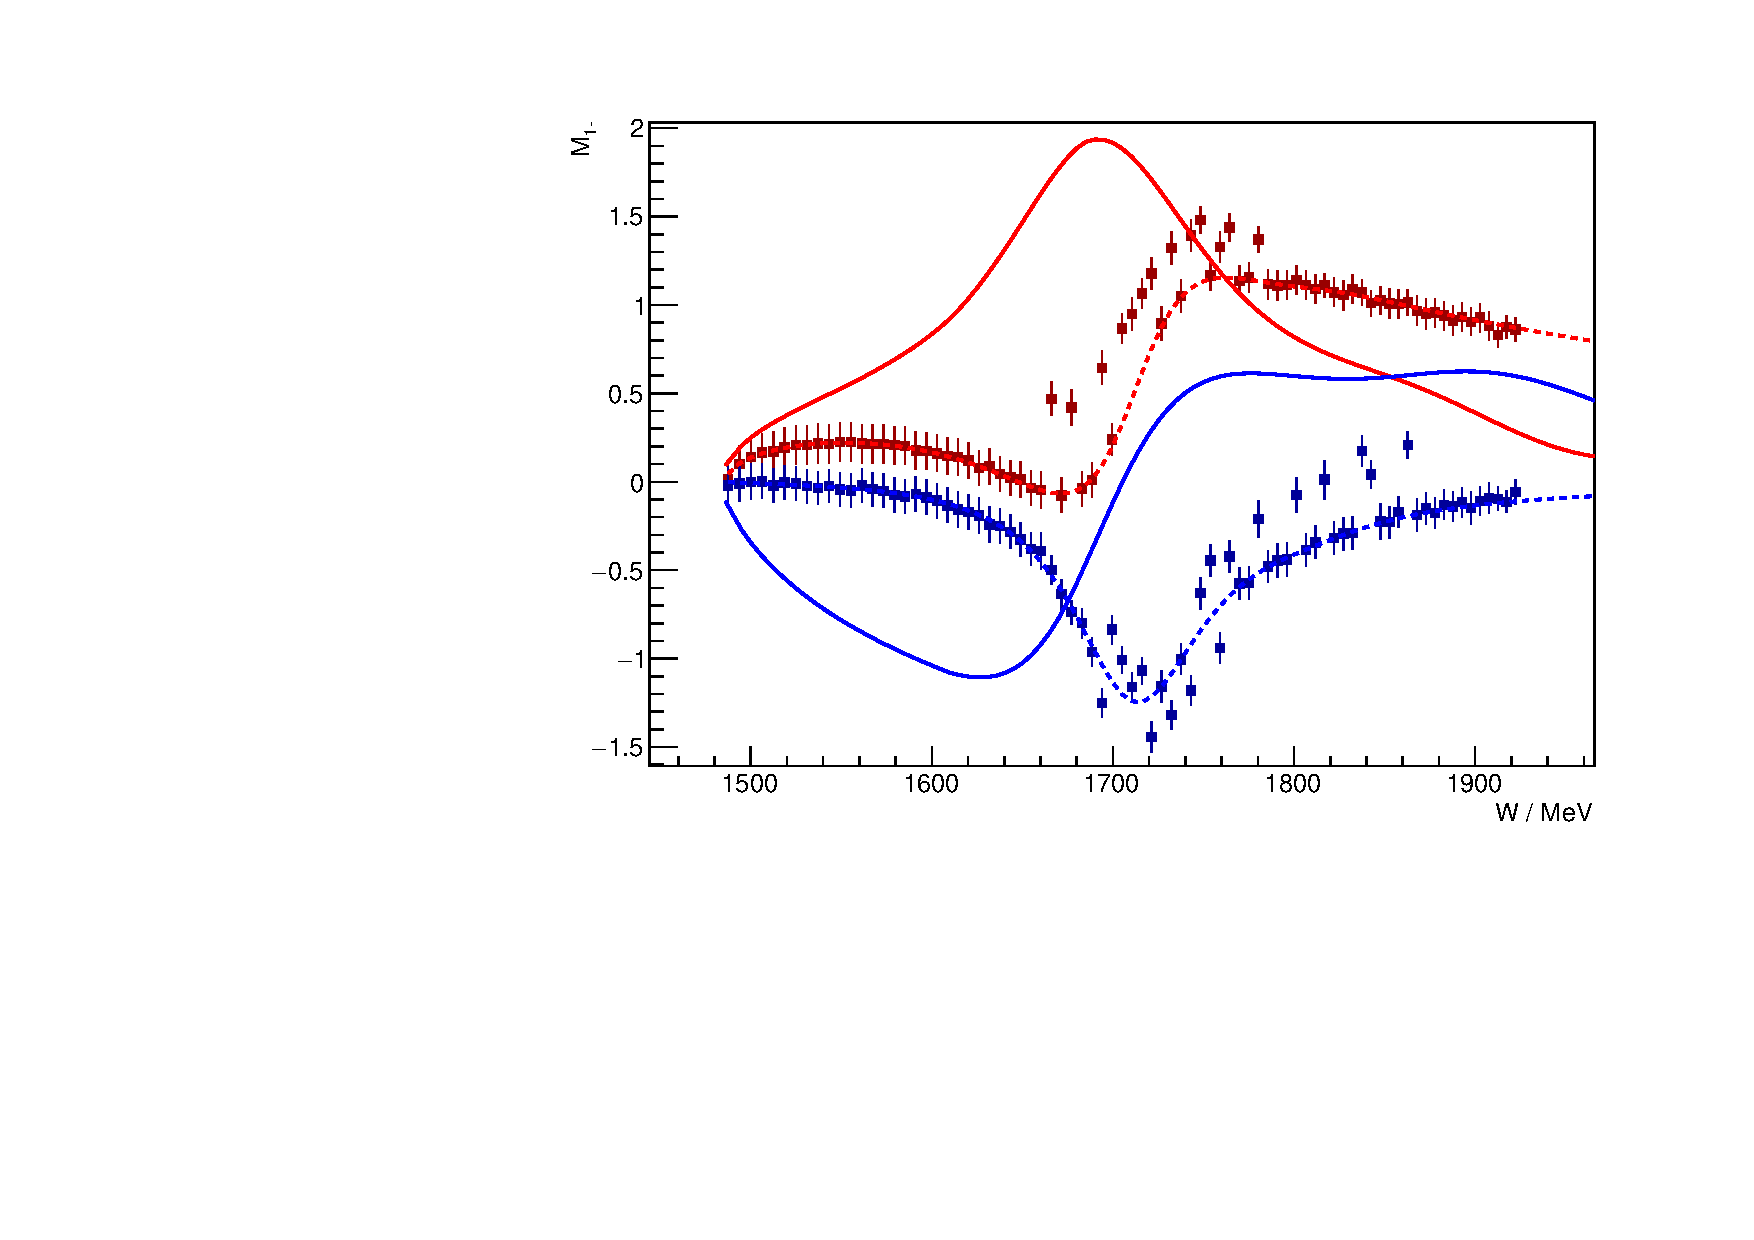
\includegraphics[width=0.49\textwidth]{BnGa/PenHeli/plots.0/M1m.pdf}
    }
    \centerline{
    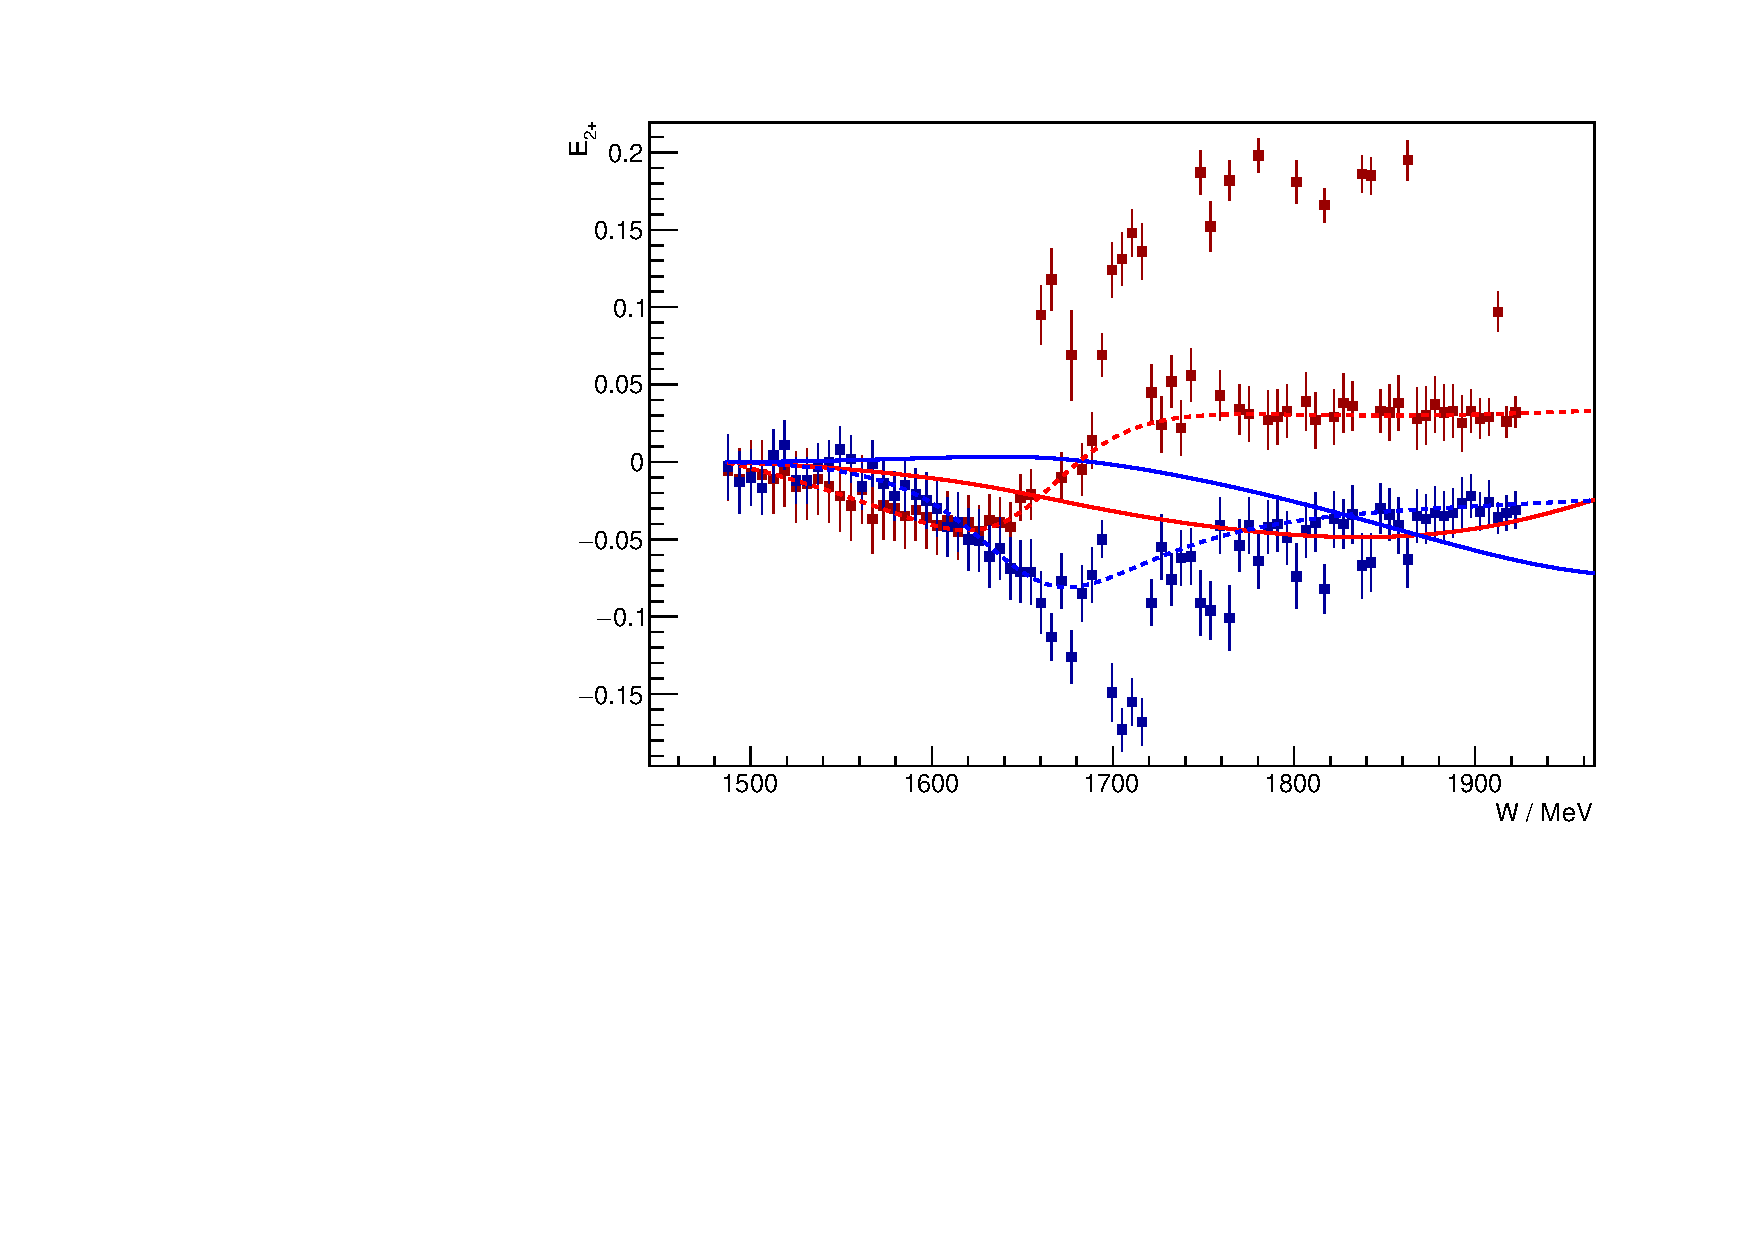
\includegraphics[width=0.49\textwidth]{BnGa/PenHeli/plots.0/E2p.pdf}
    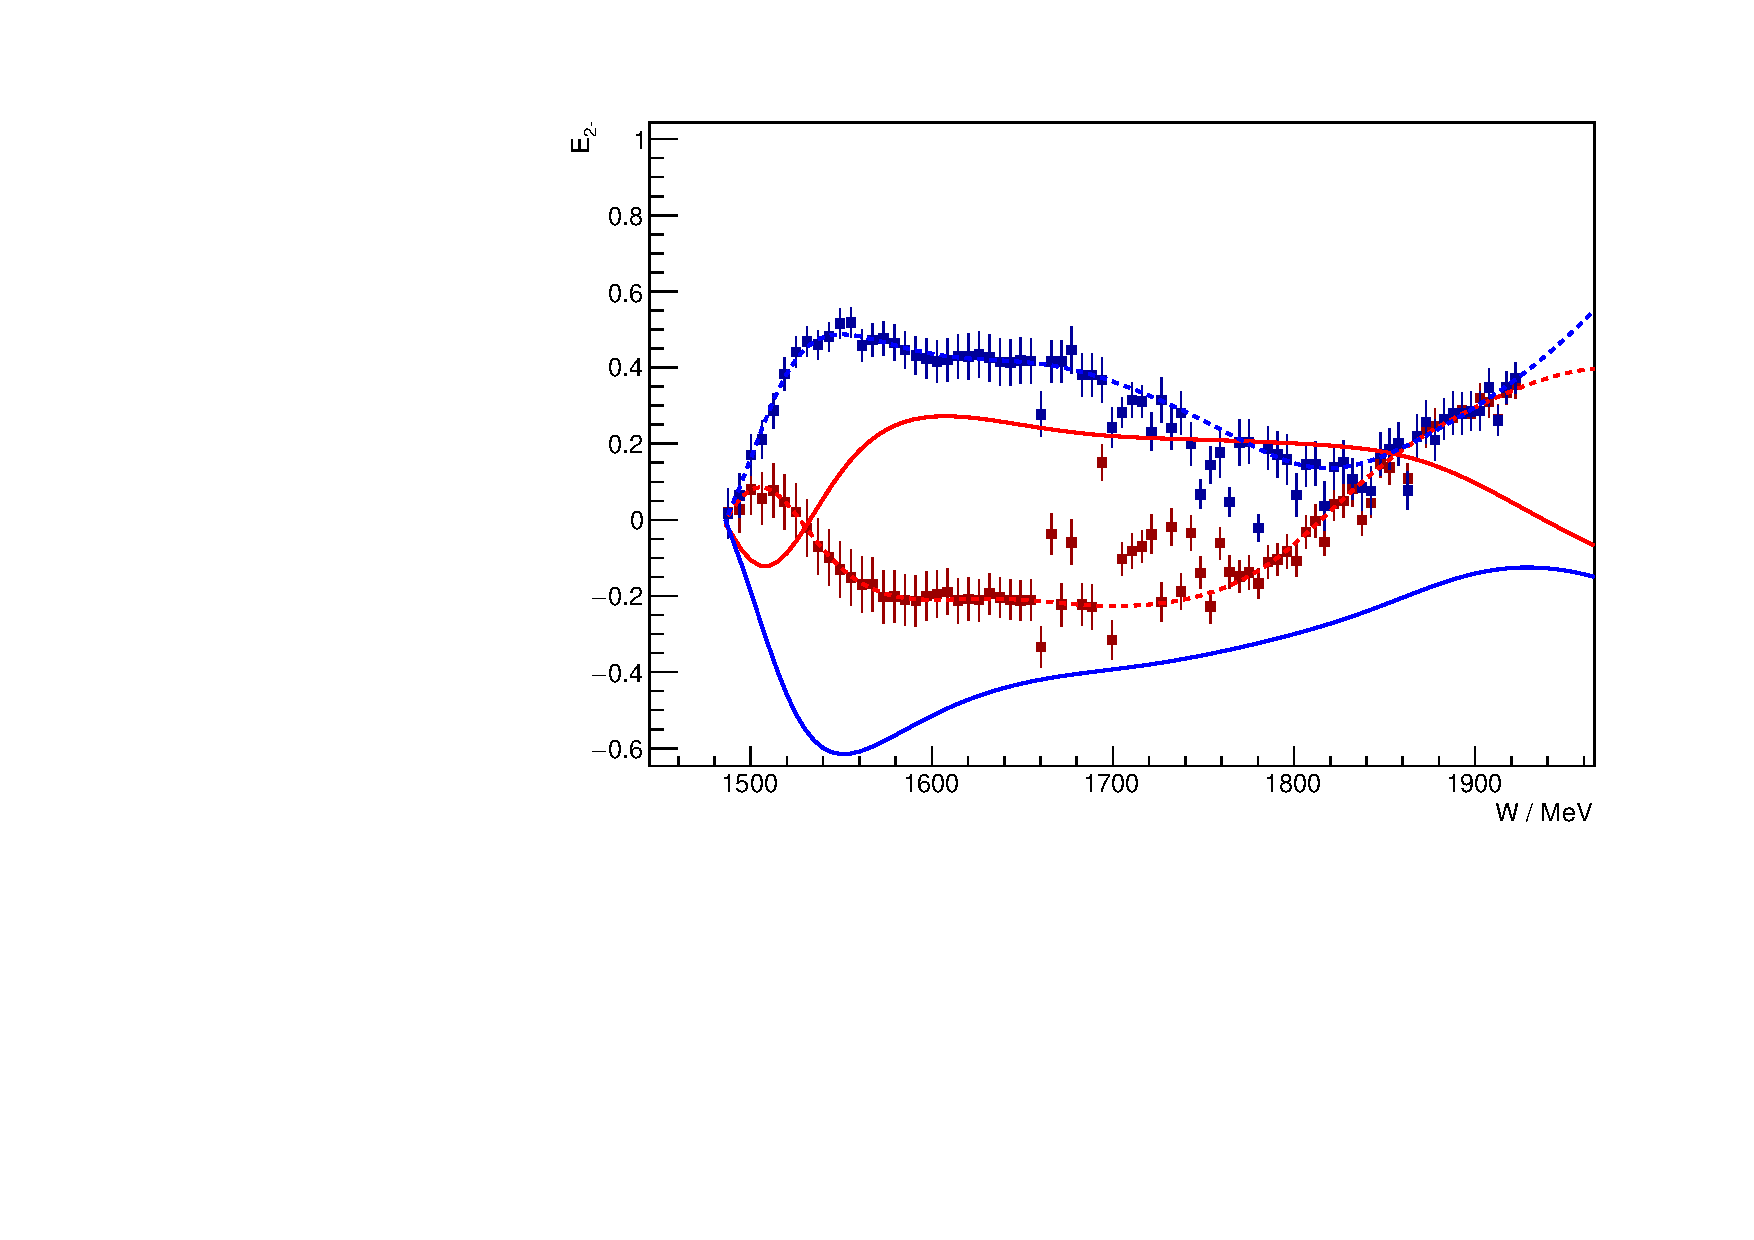
\includegraphics[width=0.49\textwidth]{BnGa/PenHeli/plots.0/E2m.pdf}
    }
    \centerline{
    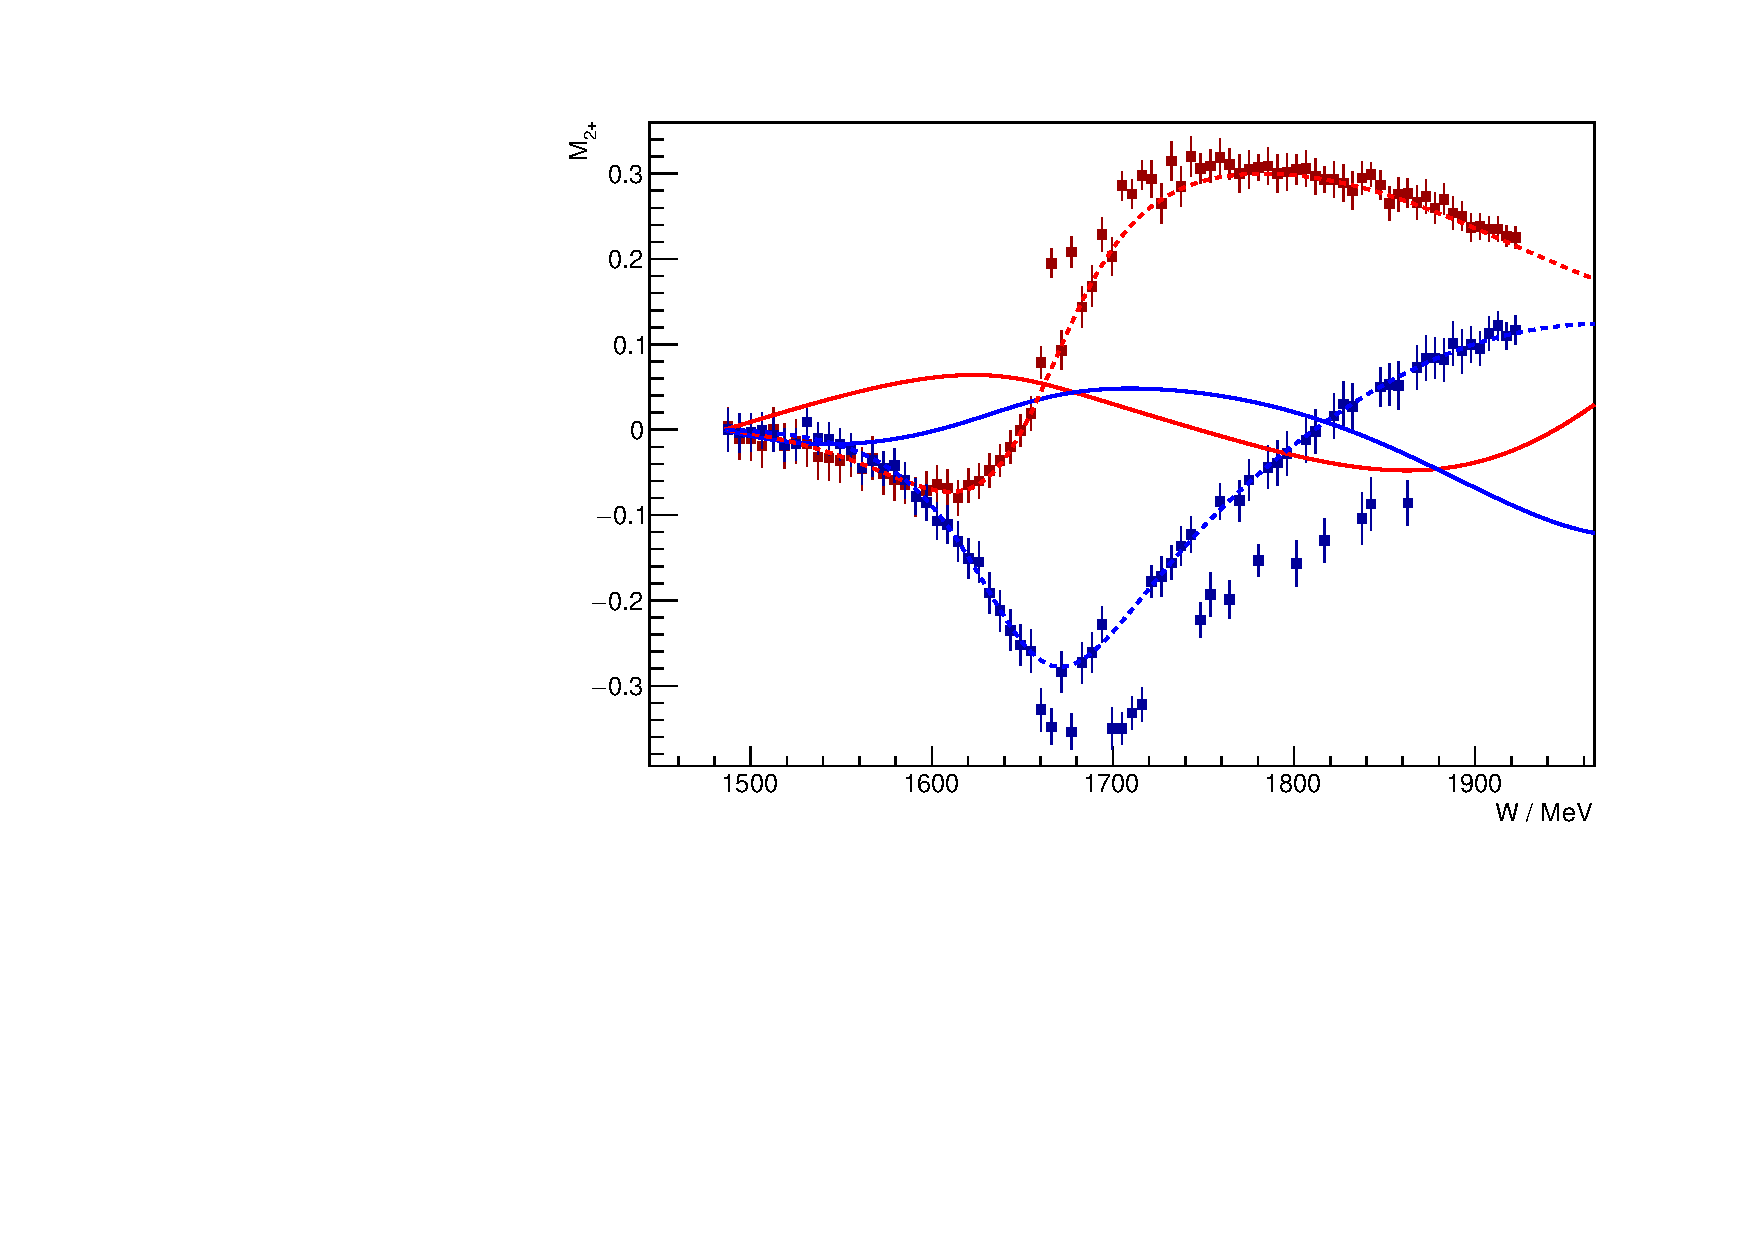
\includegraphics[width=0.49\textwidth]{BnGa/PenHeli/plots.0/M2p.pdf}
    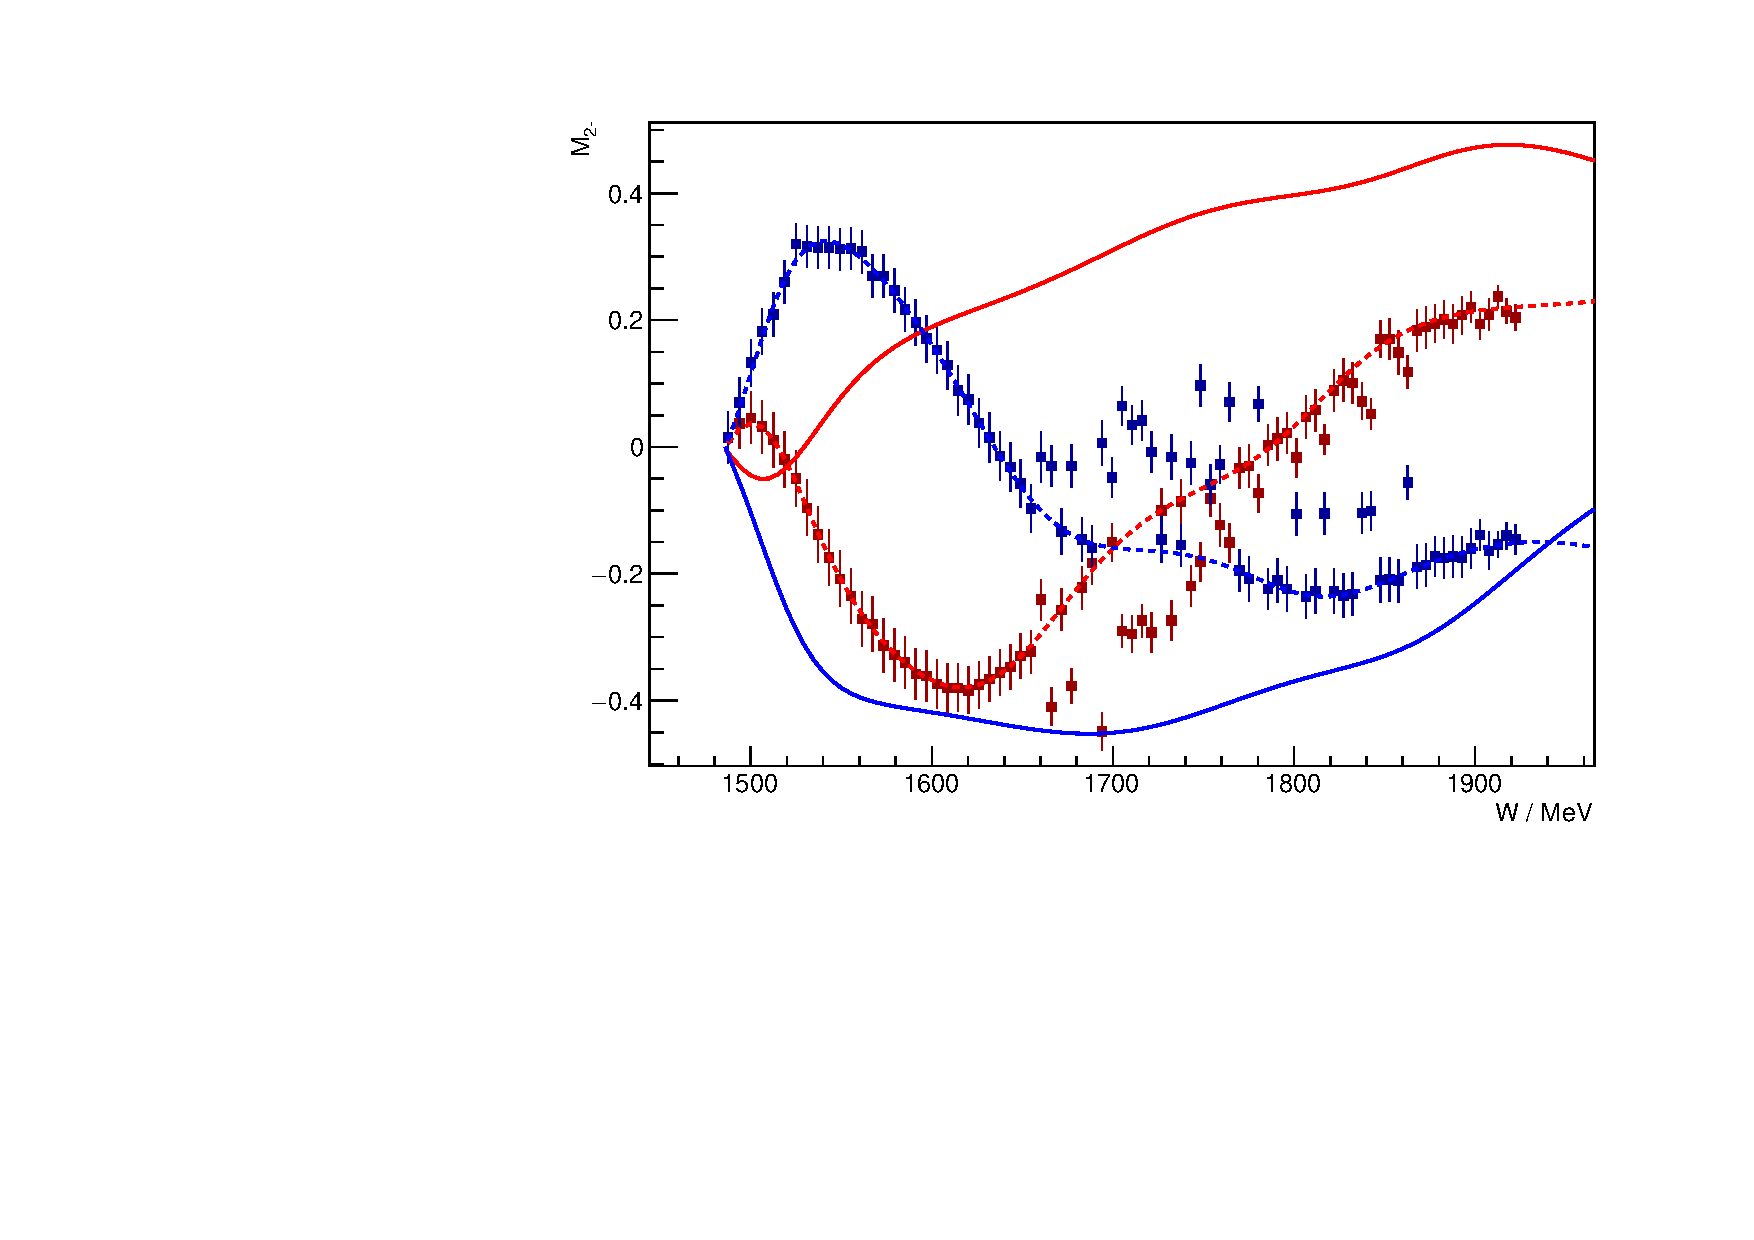
\includegraphics[width=0.49\textwidth]{BnGa/PenHeli/plots.0/M2m.pdf}
    }
    \caption{s-, p- and d-wave multipoles from a fit constrained to the "true" MAID2015a helicity amplitudes. 
    Starting values: 50\% range around the BnGa solution (solid line). The "true" MAID2015a curves are
    shown by the dashed lines.}
\label{Fig:const2}
  \end{center}
\end{figure}

\begin{figure}
  \begin{center}
    \centerline{
    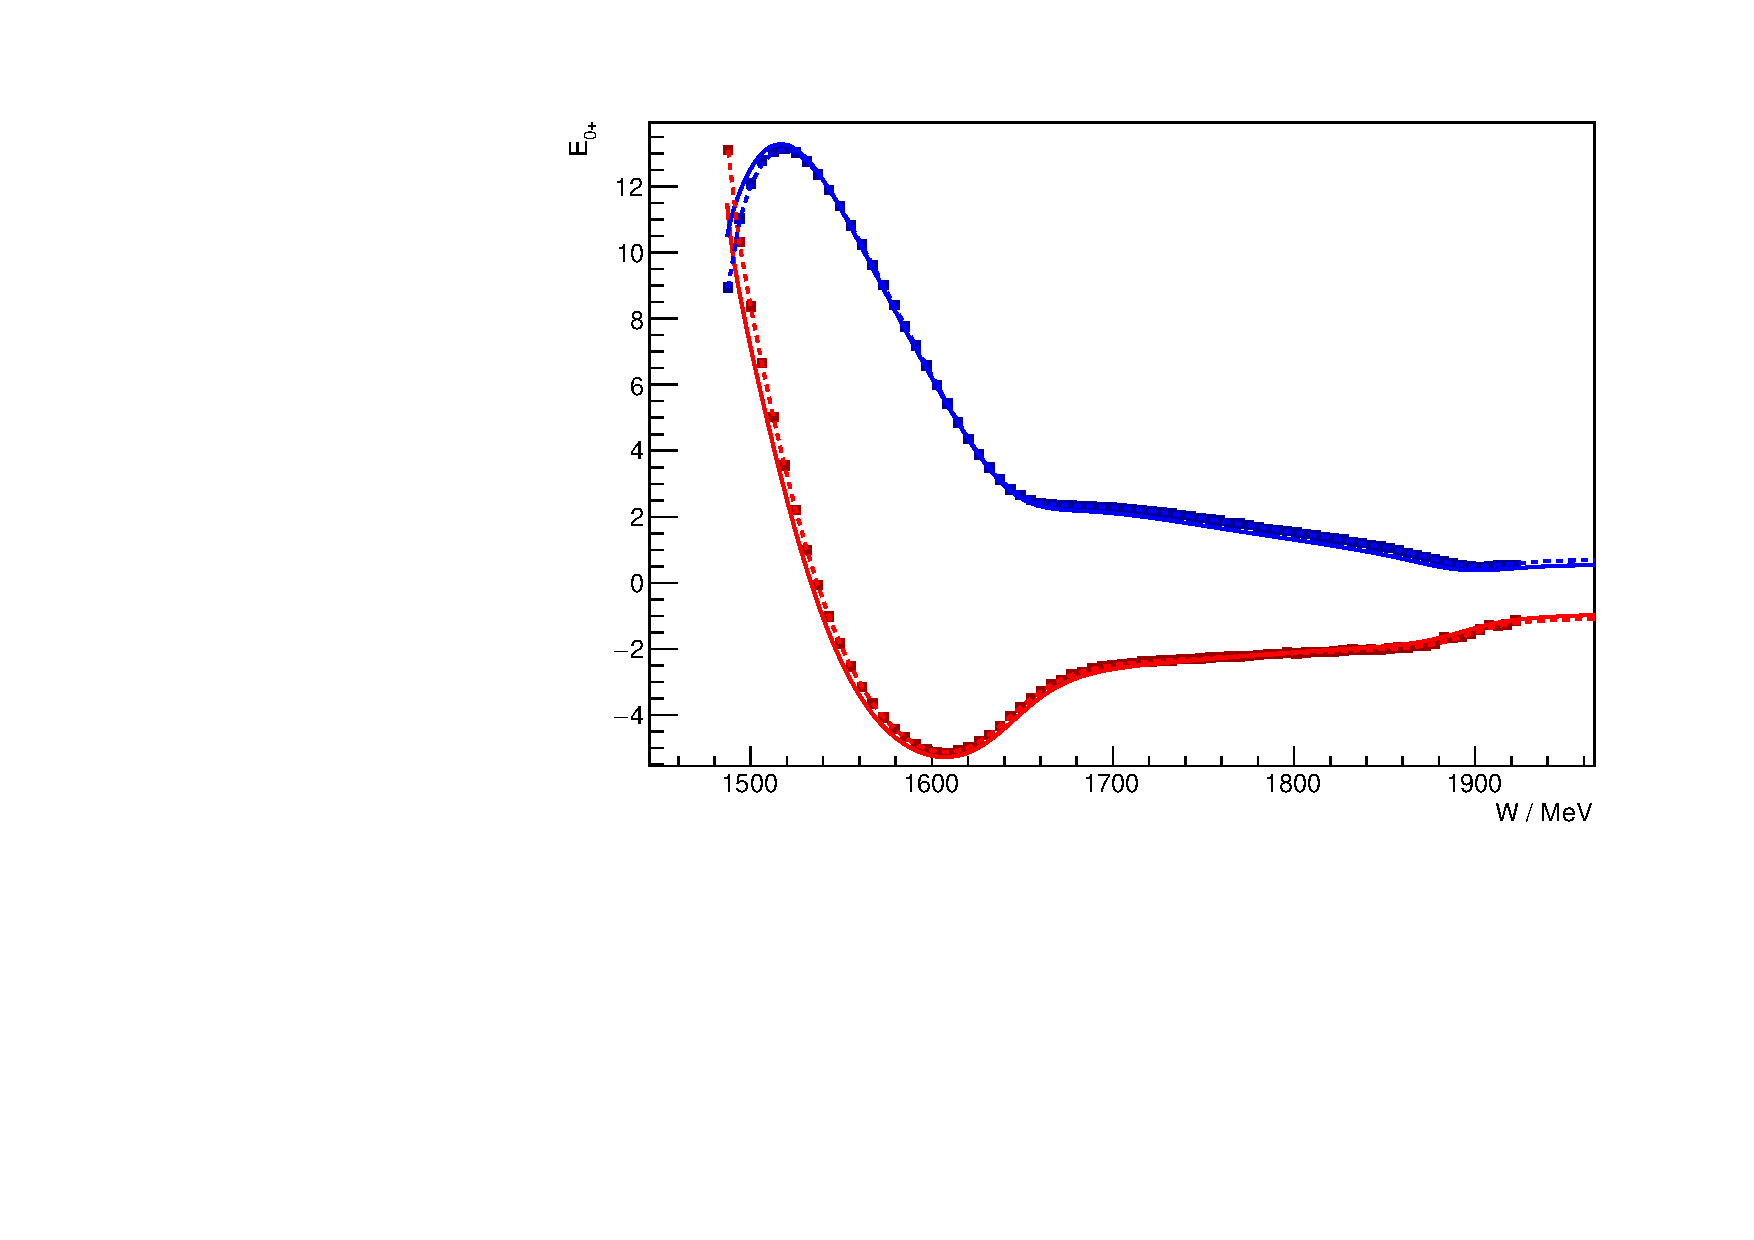
\includegraphics[width=0.49\textwidth]{MAID/PenHeli/plots.0/E0p.pdf}
    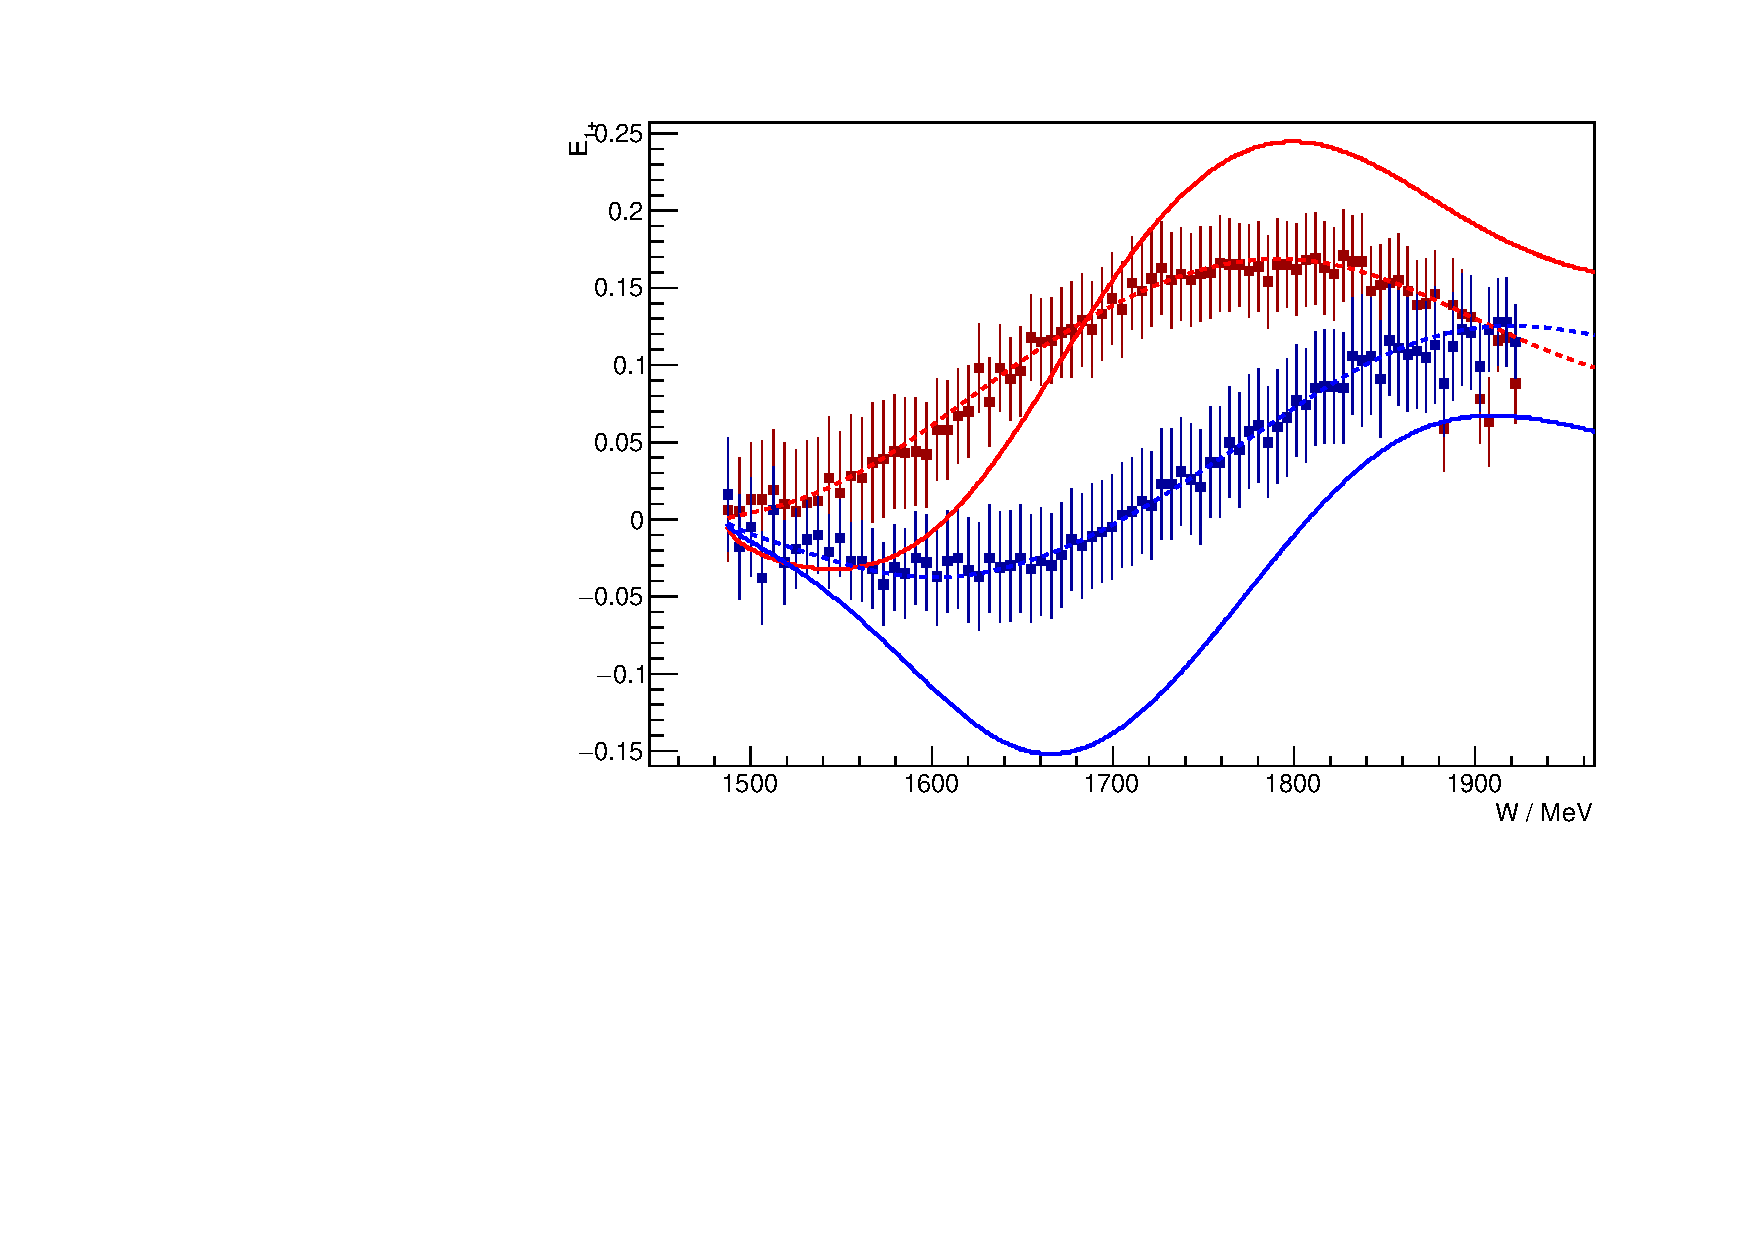
\includegraphics[width=0.49\textwidth]{MAID/PenHeli/plots.0/E1p.pdf}
    }
    \centerline{
    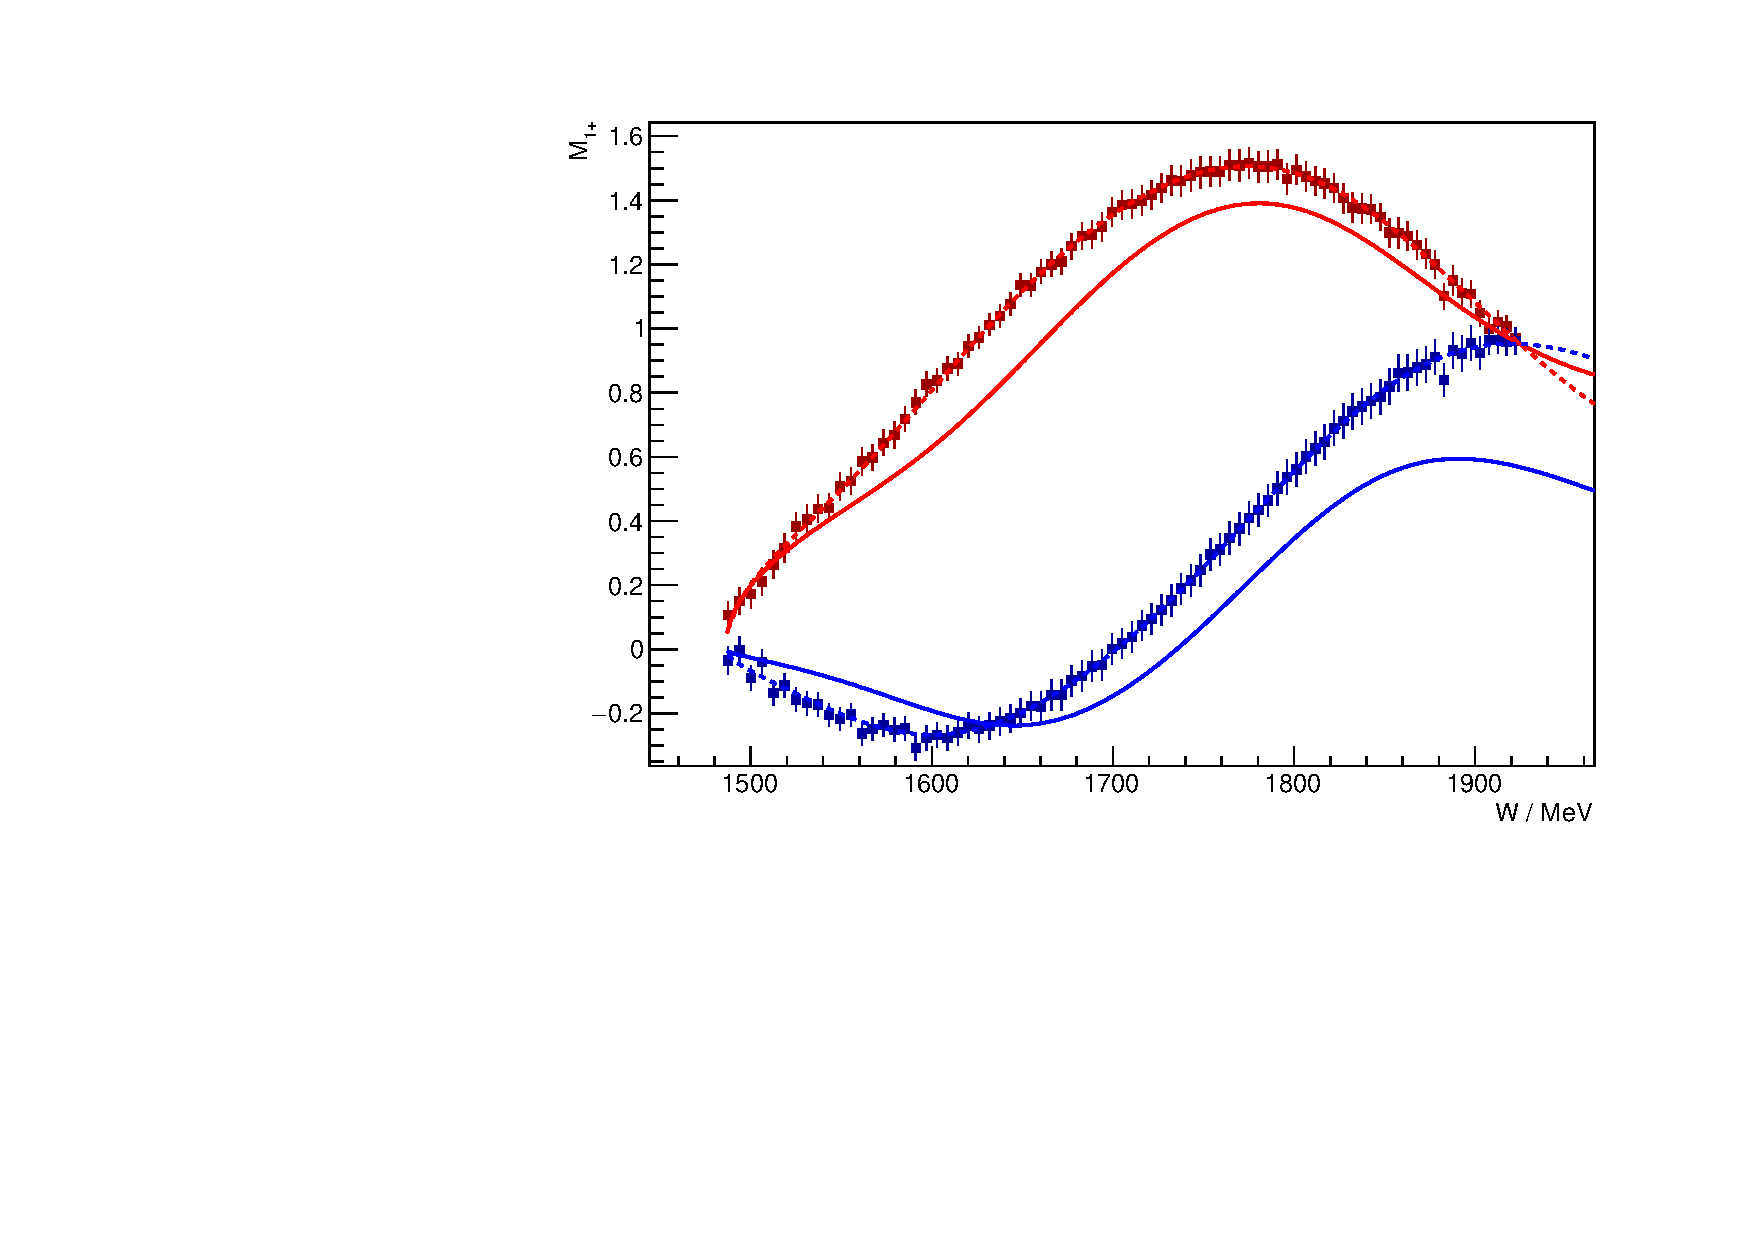
\includegraphics[width=0.49\textwidth]{MAID/PenHeli/plots.0/M1p.pdf}
    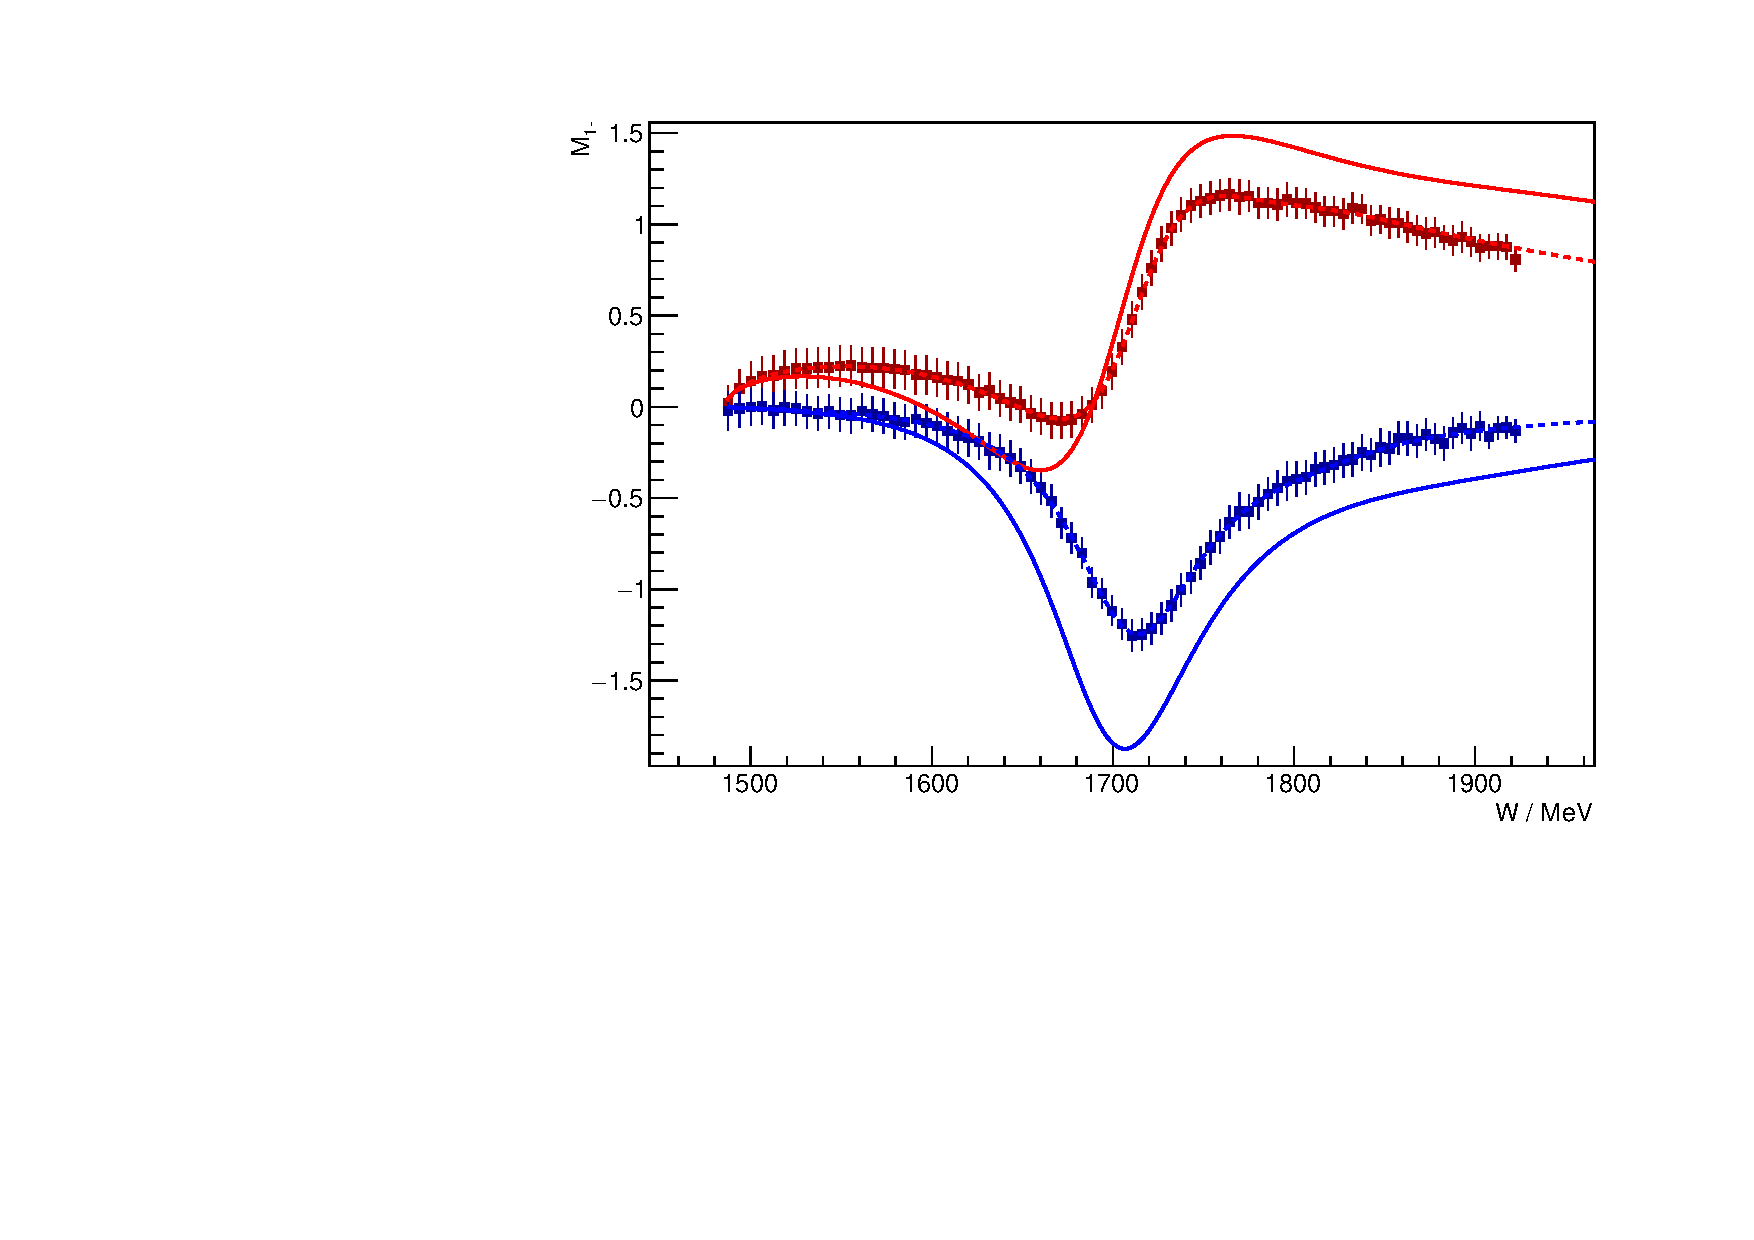
\includegraphics[width=0.49\textwidth]{MAID/PenHeli/plots.0/M1m.pdf}
    }
    \centerline{
    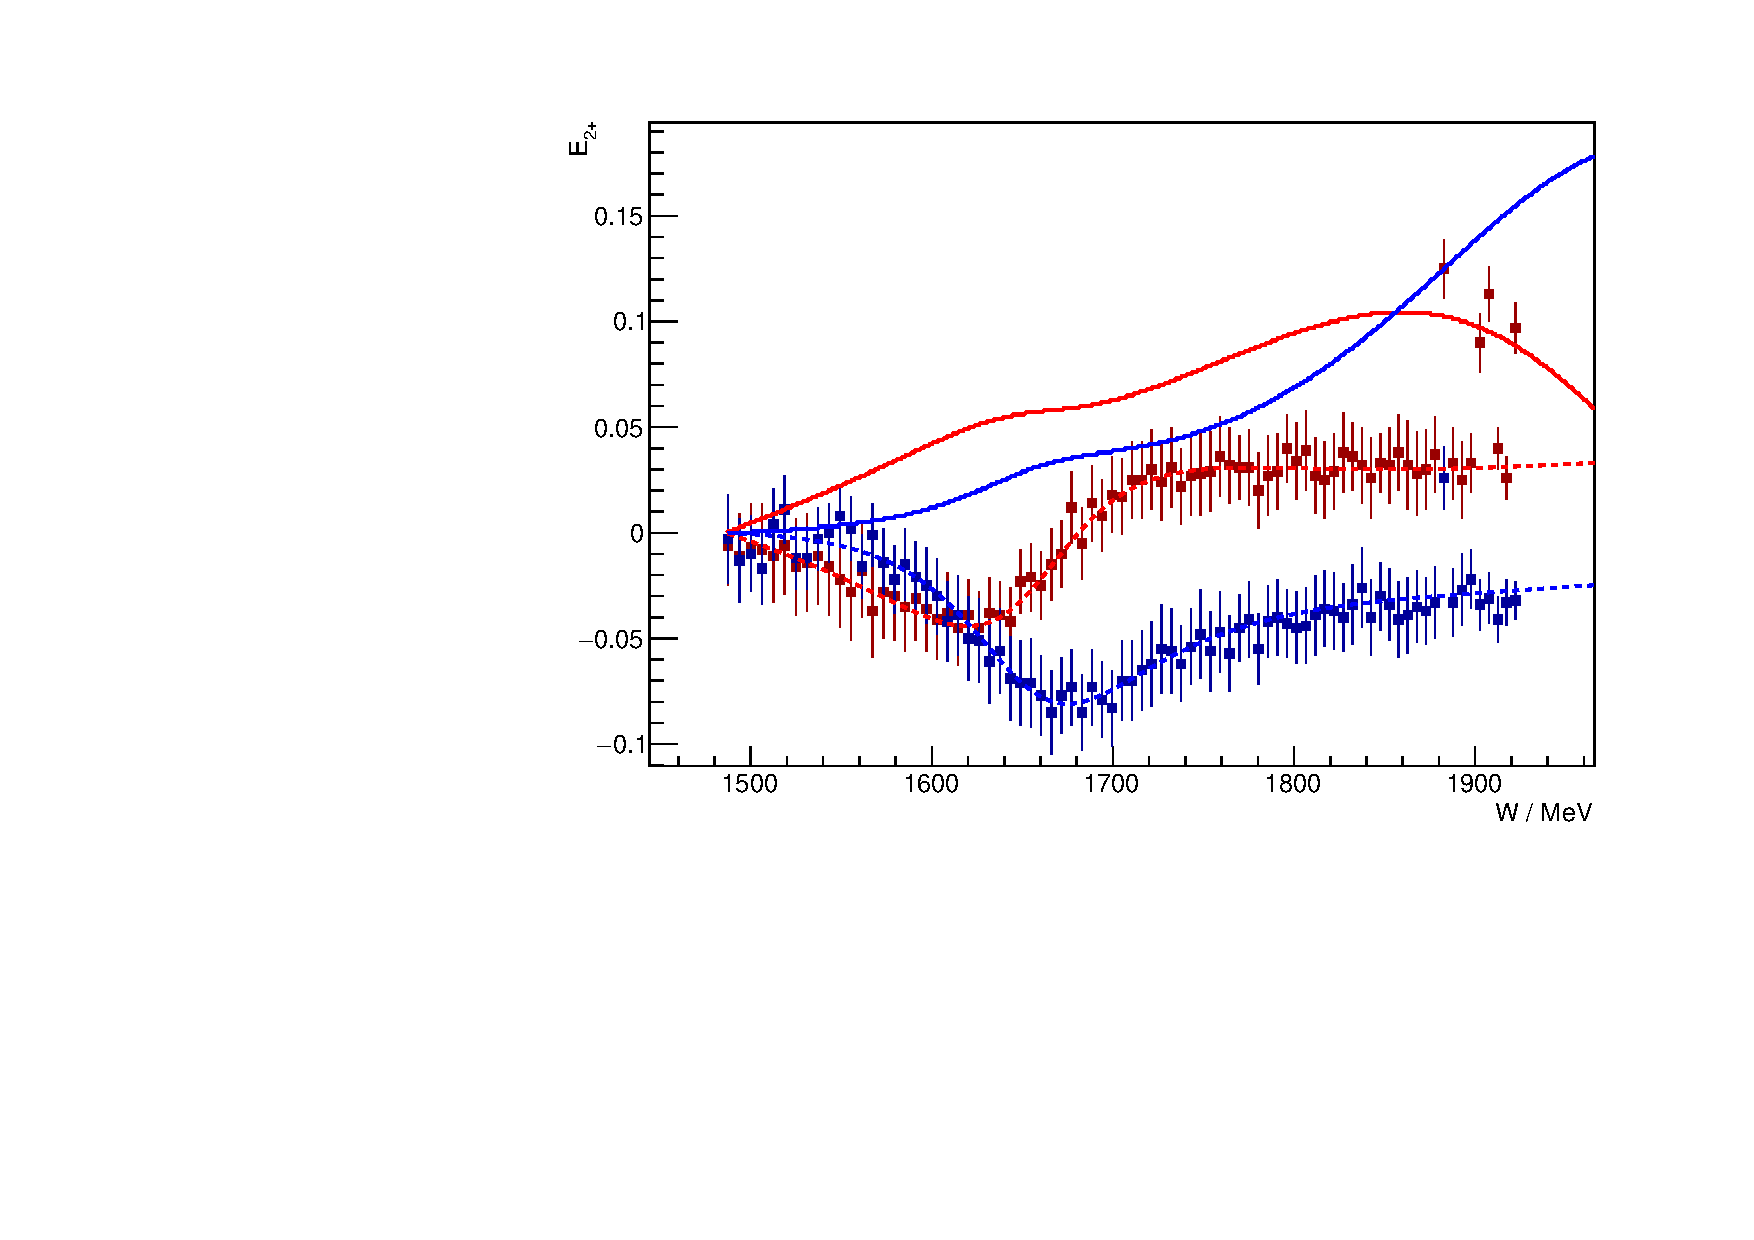
\includegraphics[width=0.49\textwidth]{MAID/PenHeli/plots.0/E2p.pdf}
    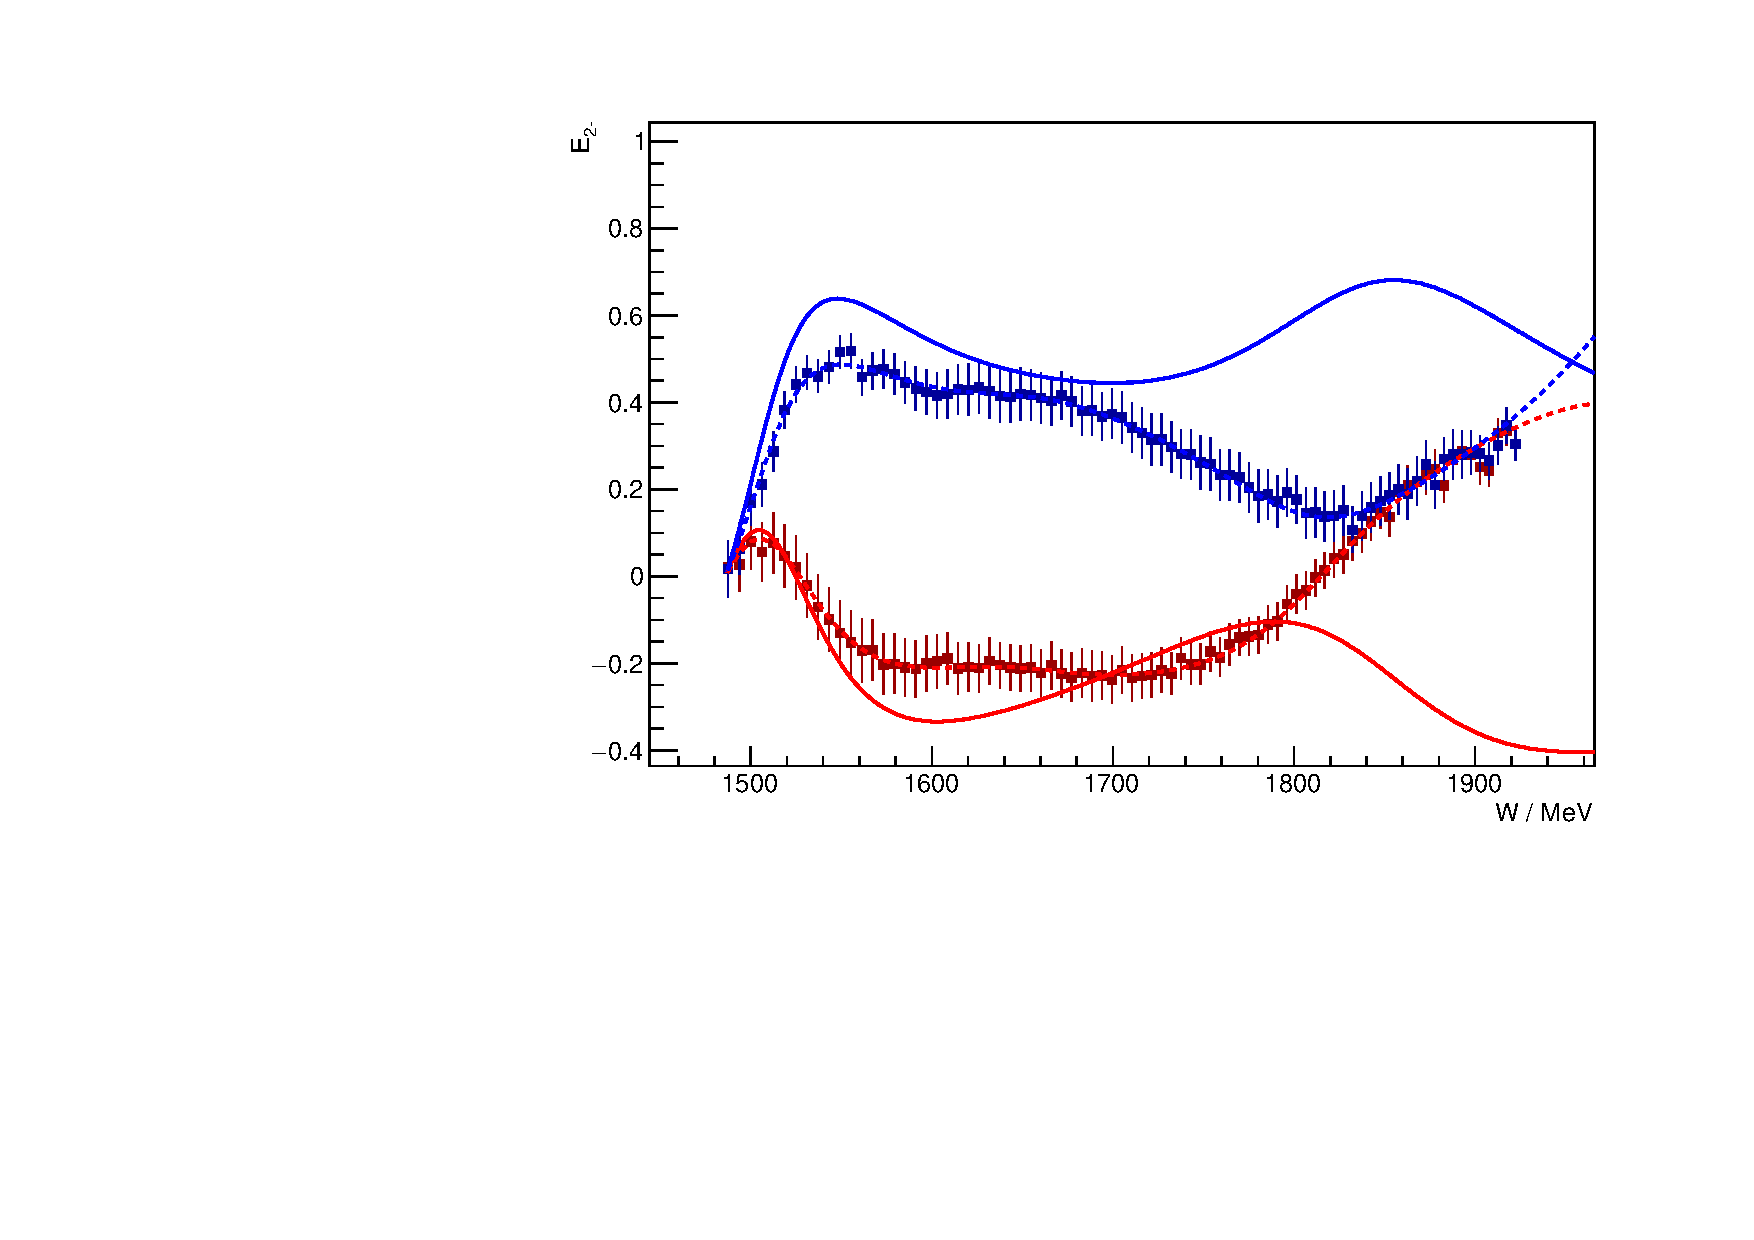
\includegraphics[width=0.49\textwidth]{MAID/PenHeli/plots.0/E2m.pdf}
    }
    \centerline{
    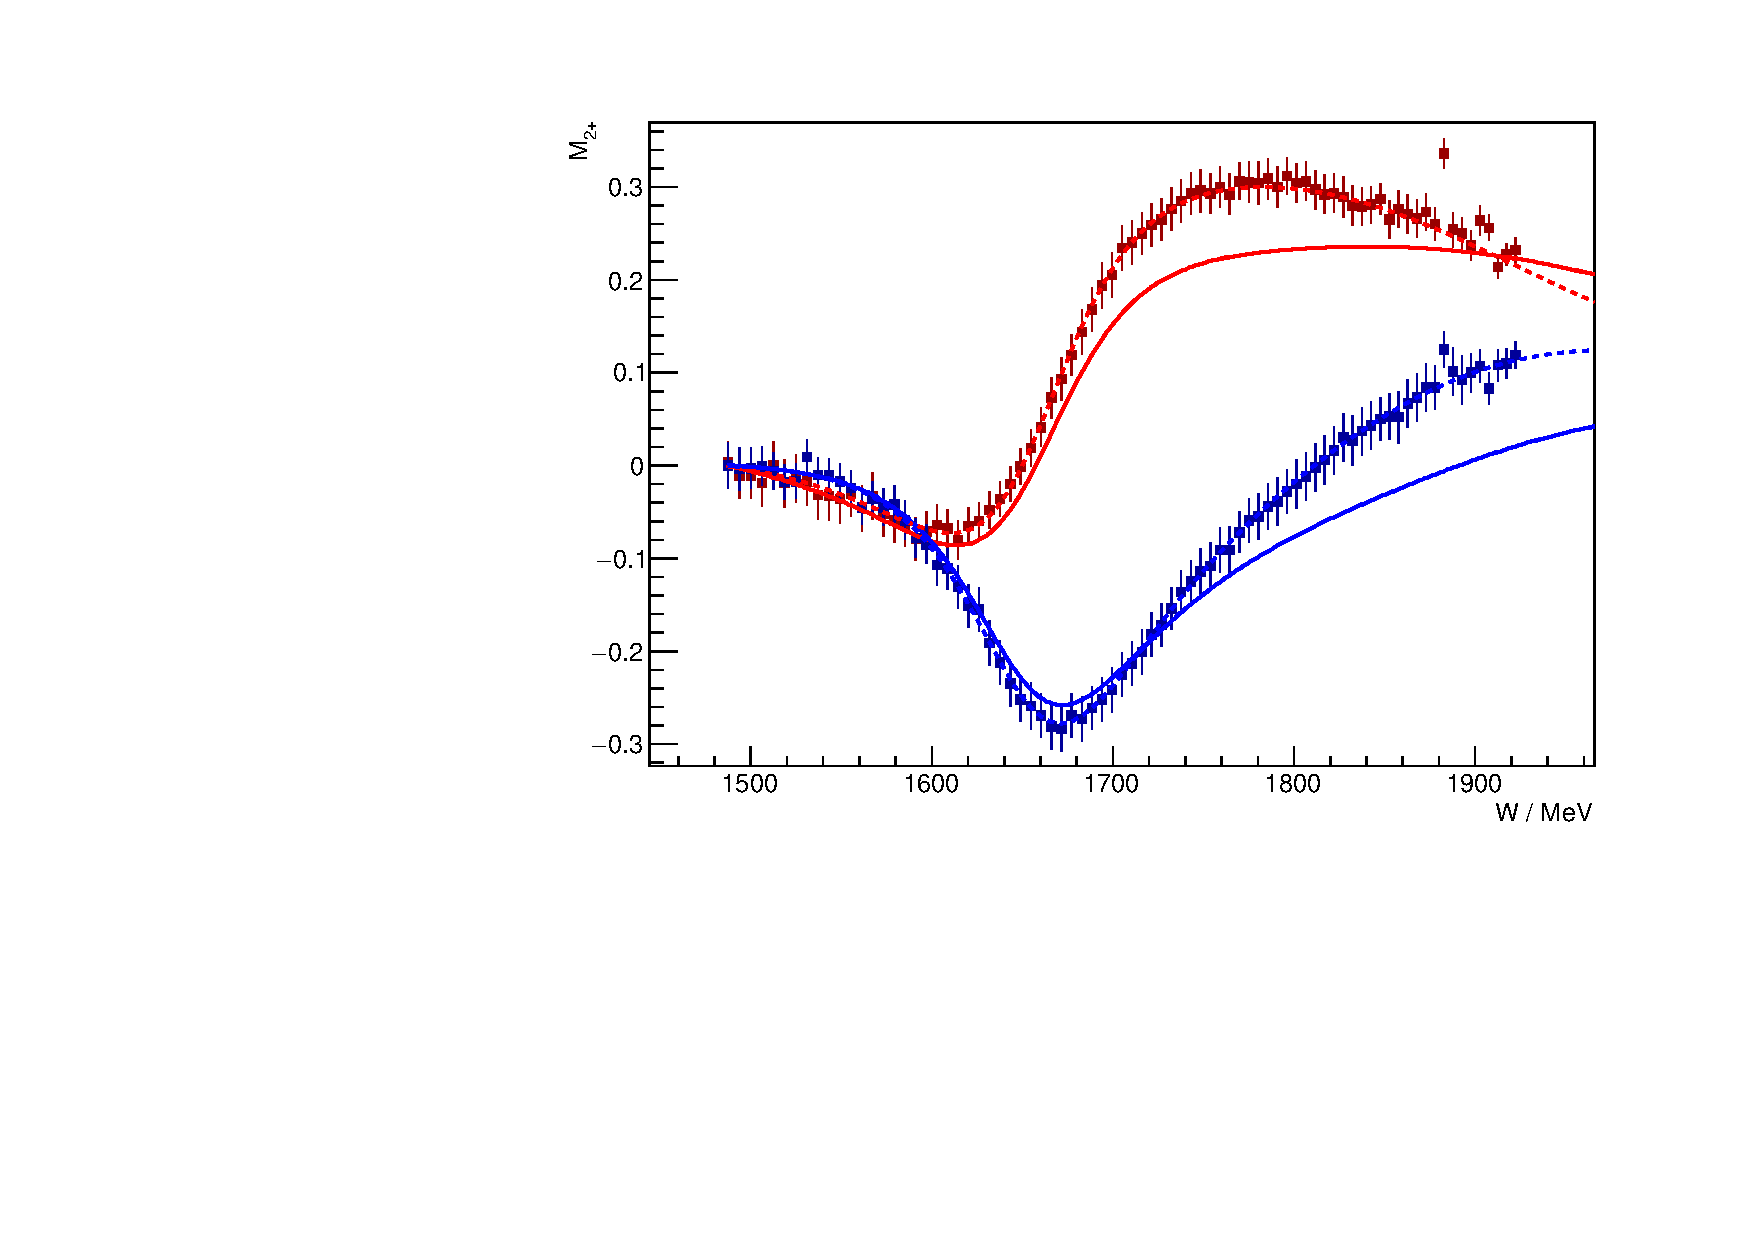
\includegraphics[width=0.49\textwidth]{MAID/PenHeli/plots.0/M2p.pdf}
    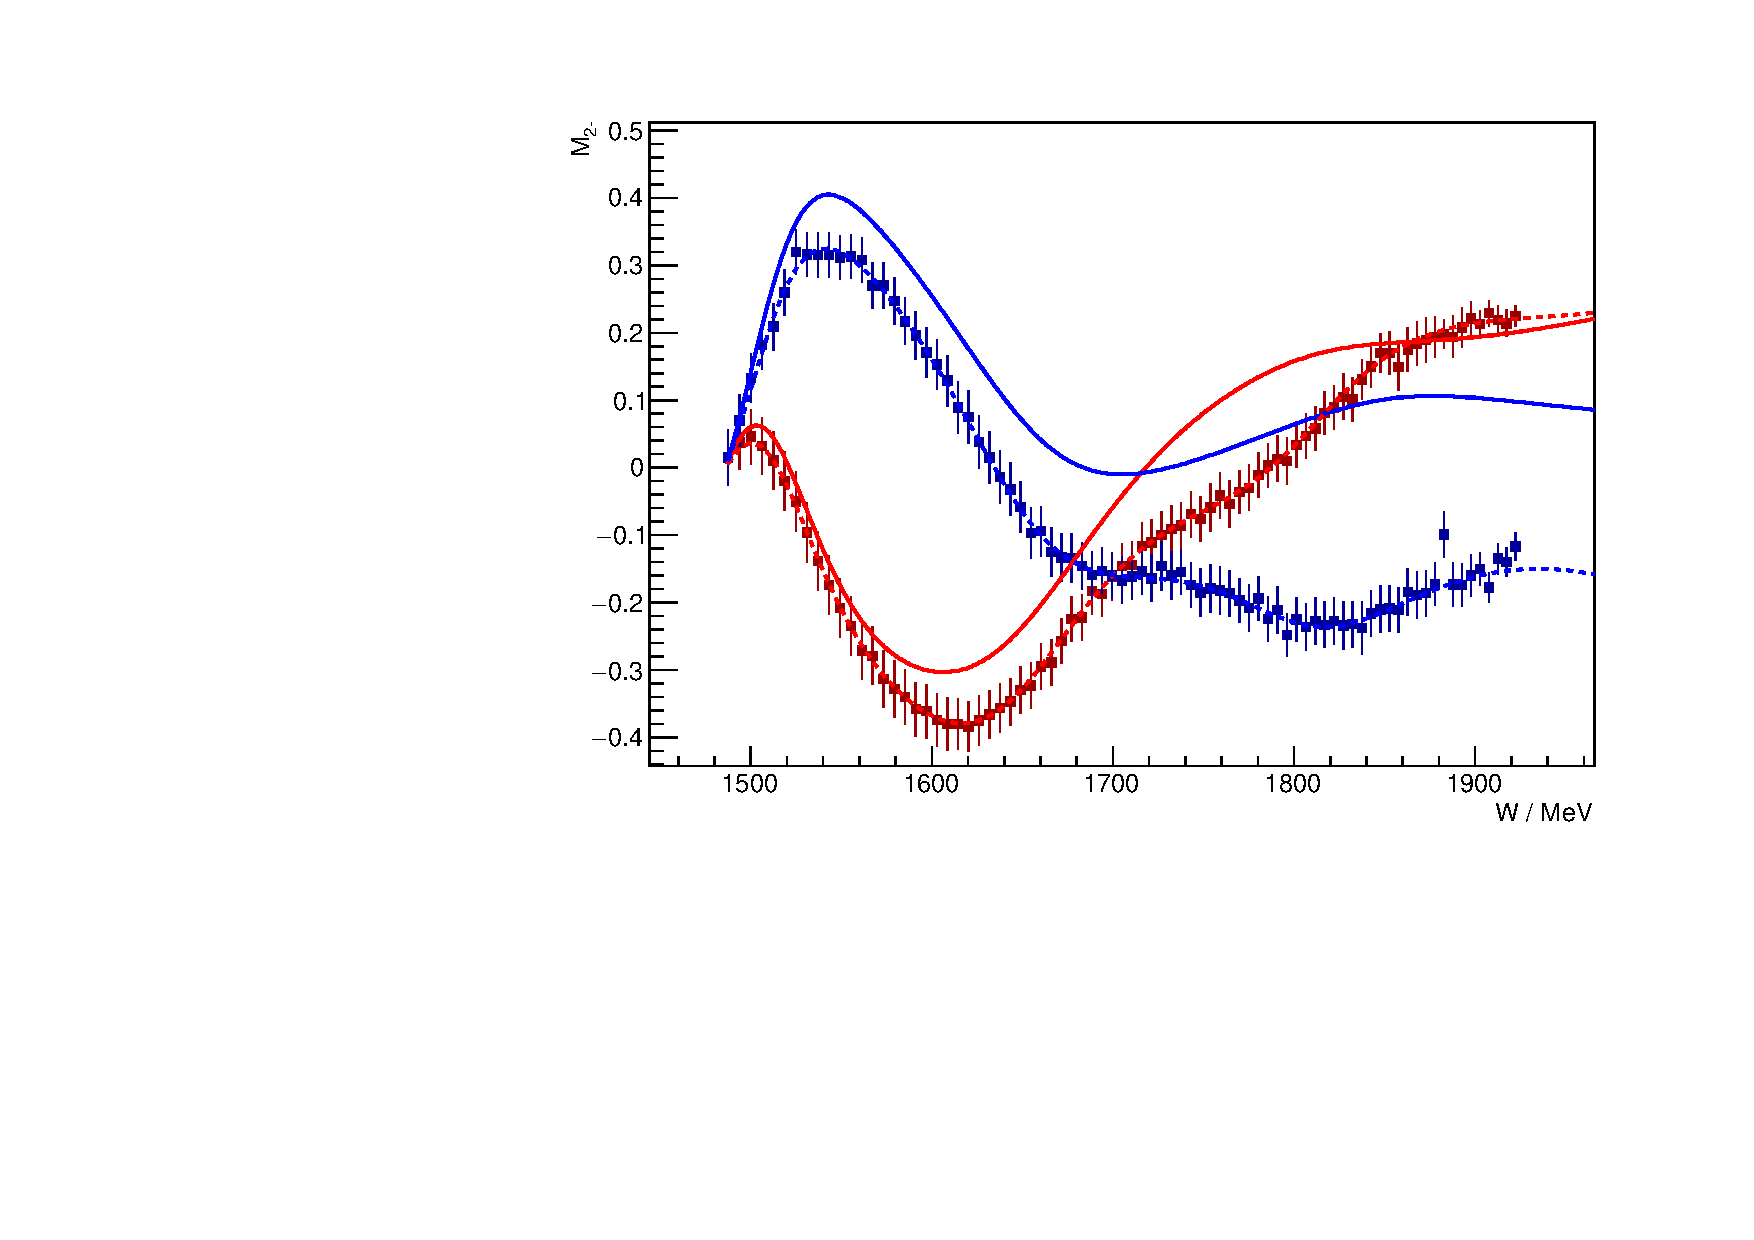
\includegraphics[width=0.49\textwidth]{MAID/PenHeli/plots.0/M2m.pdf}
    }
    \caption{s-, p- and d-wave multipoles from a fit constrained to the "true" MAID2015a helicity amplitudes. 
    Starting values: 50\% range around the $\eta$-MAID2003 solution (solid line). The "true" MAID2015a curves are
    shown by the dashed lines.}
\label{Fig:const3}
  \end{center}
\end{figure}


\begin{figure}
  \begin{center}
    \centerline{
    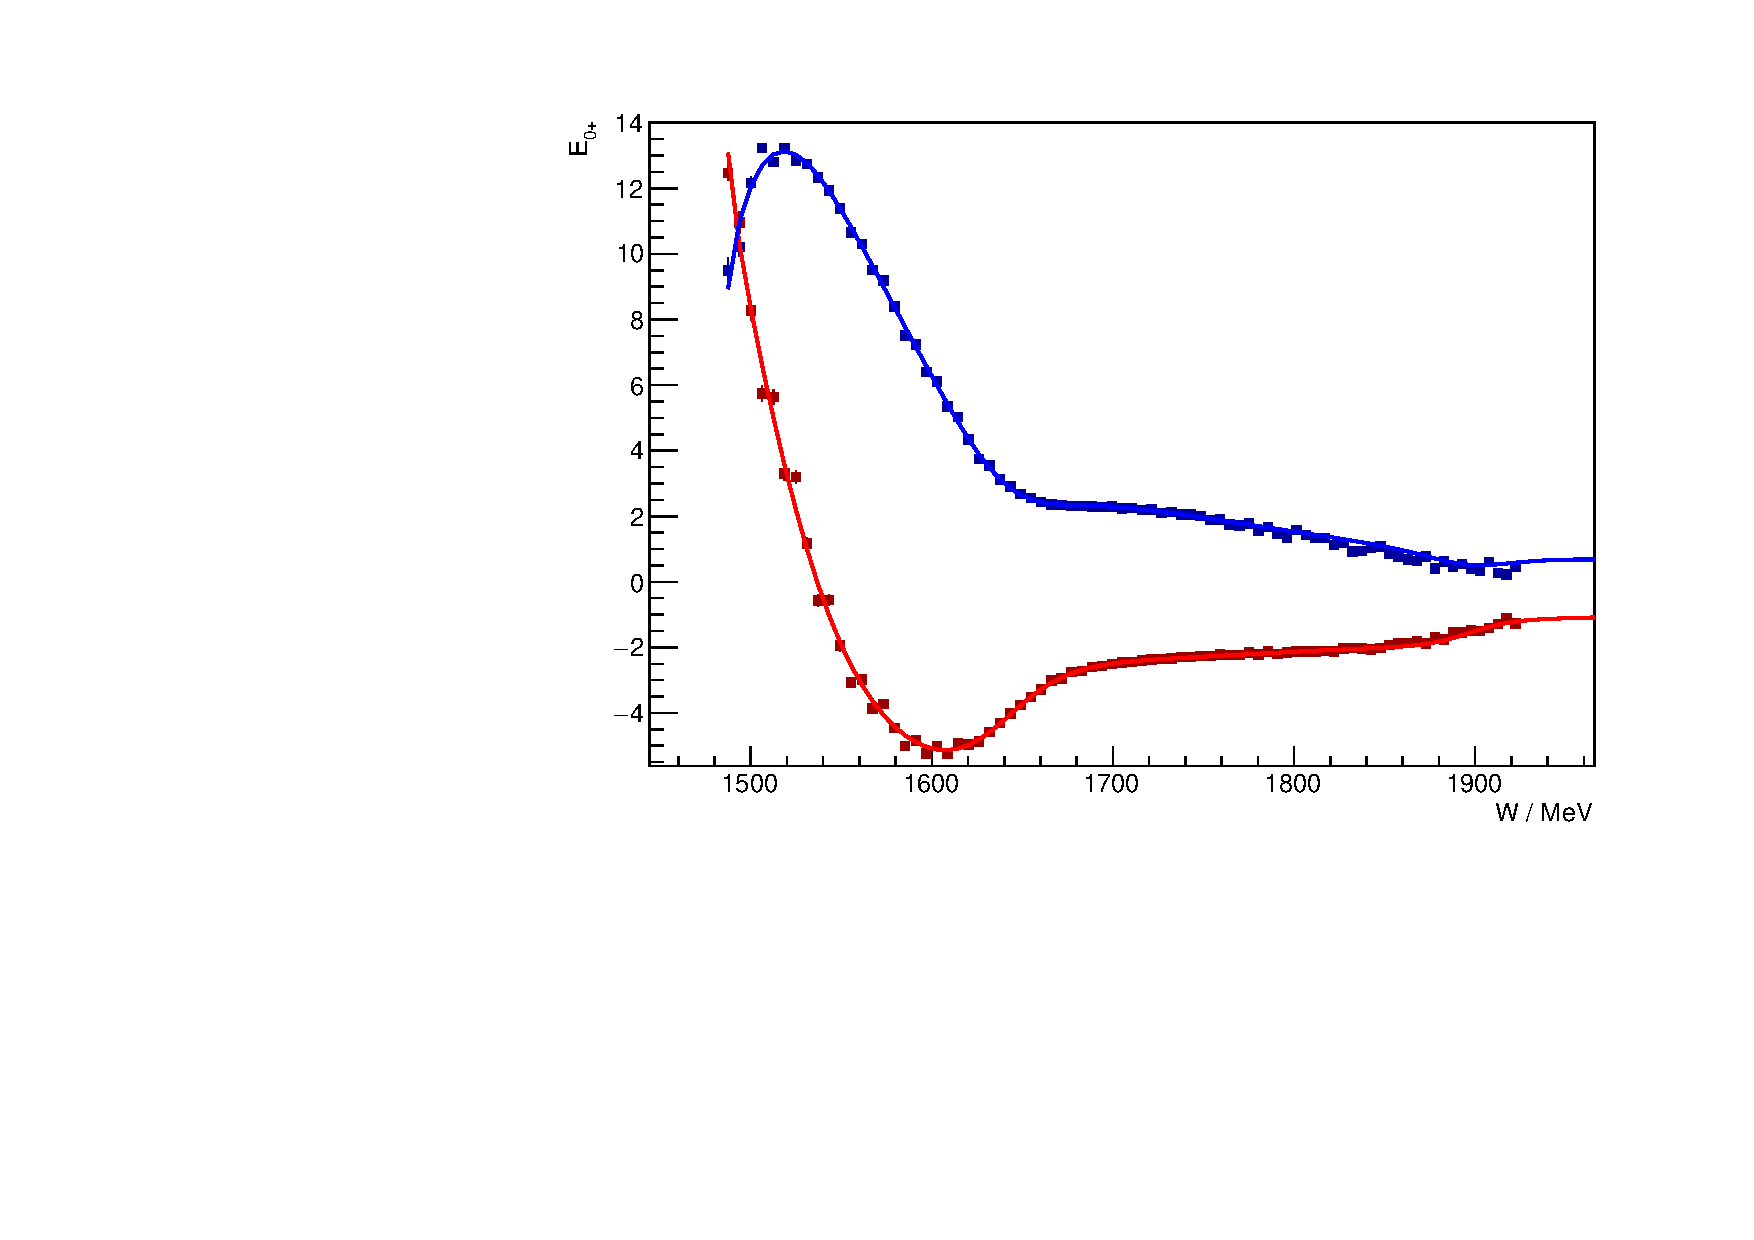
\includegraphics[width=0.49\textwidth]{MAID2015a/Hedim/plots.0/E0p.pdf}
    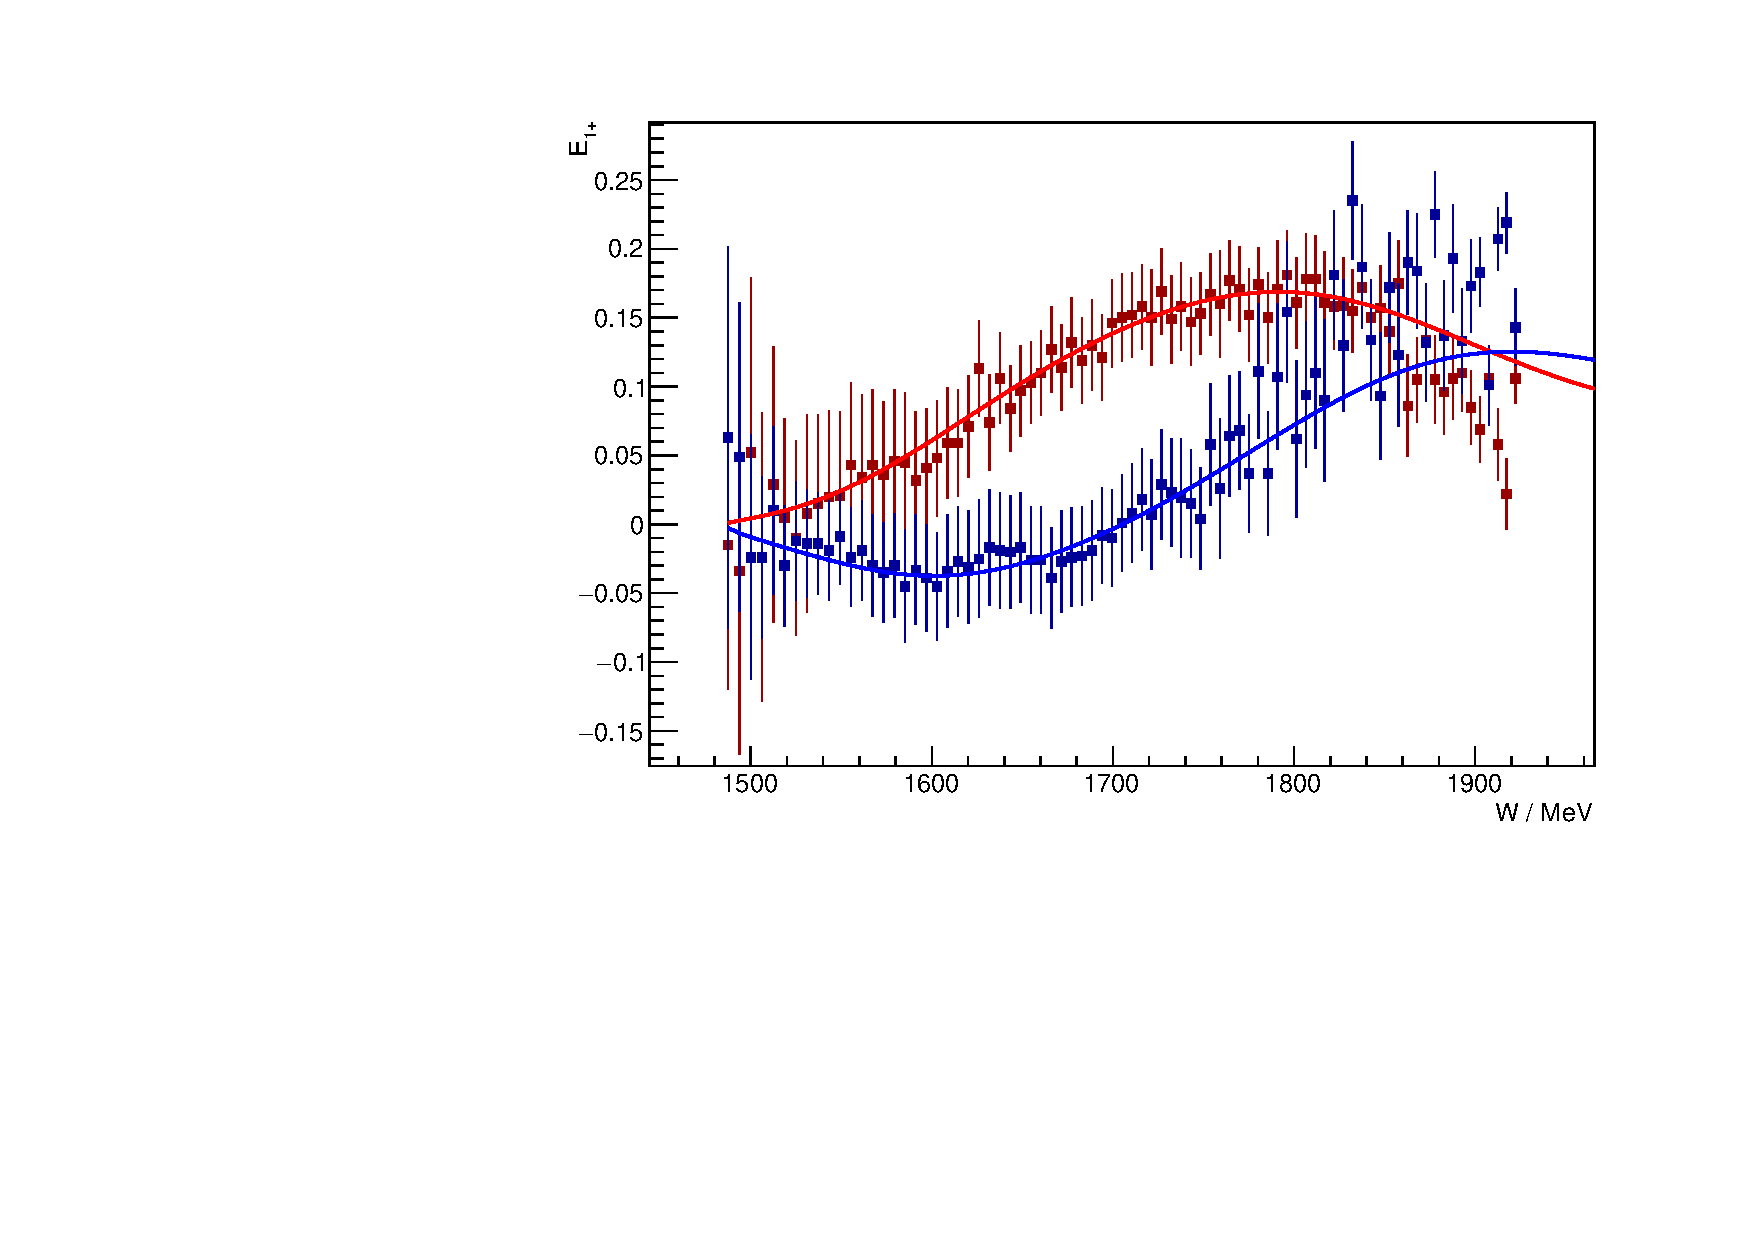
\includegraphics[width=0.49\textwidth]{MAID2015a/Hedim/plots.0/E1p.pdf}
    }
    \centerline{
    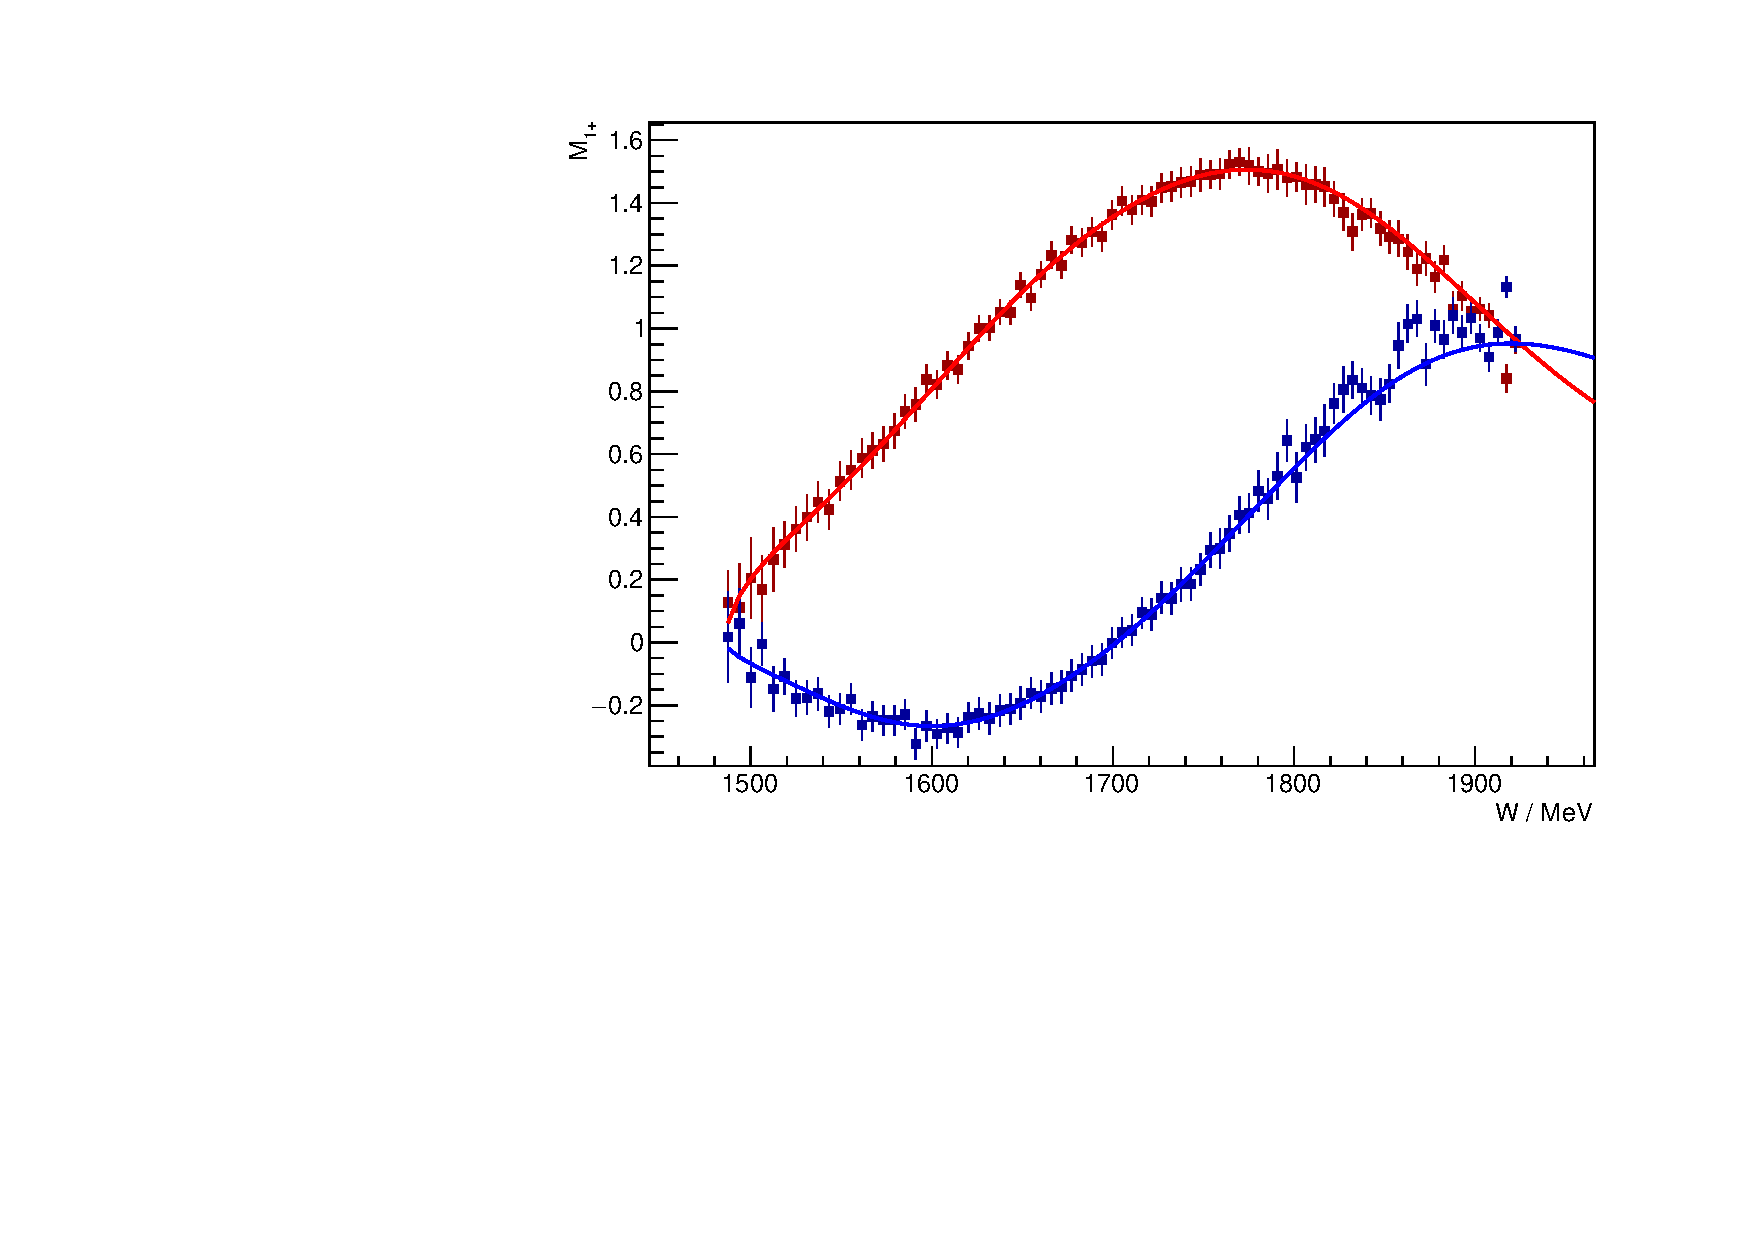
\includegraphics[width=0.49\textwidth]{MAID2015a/Hedim/plots.0/M1p.pdf}
    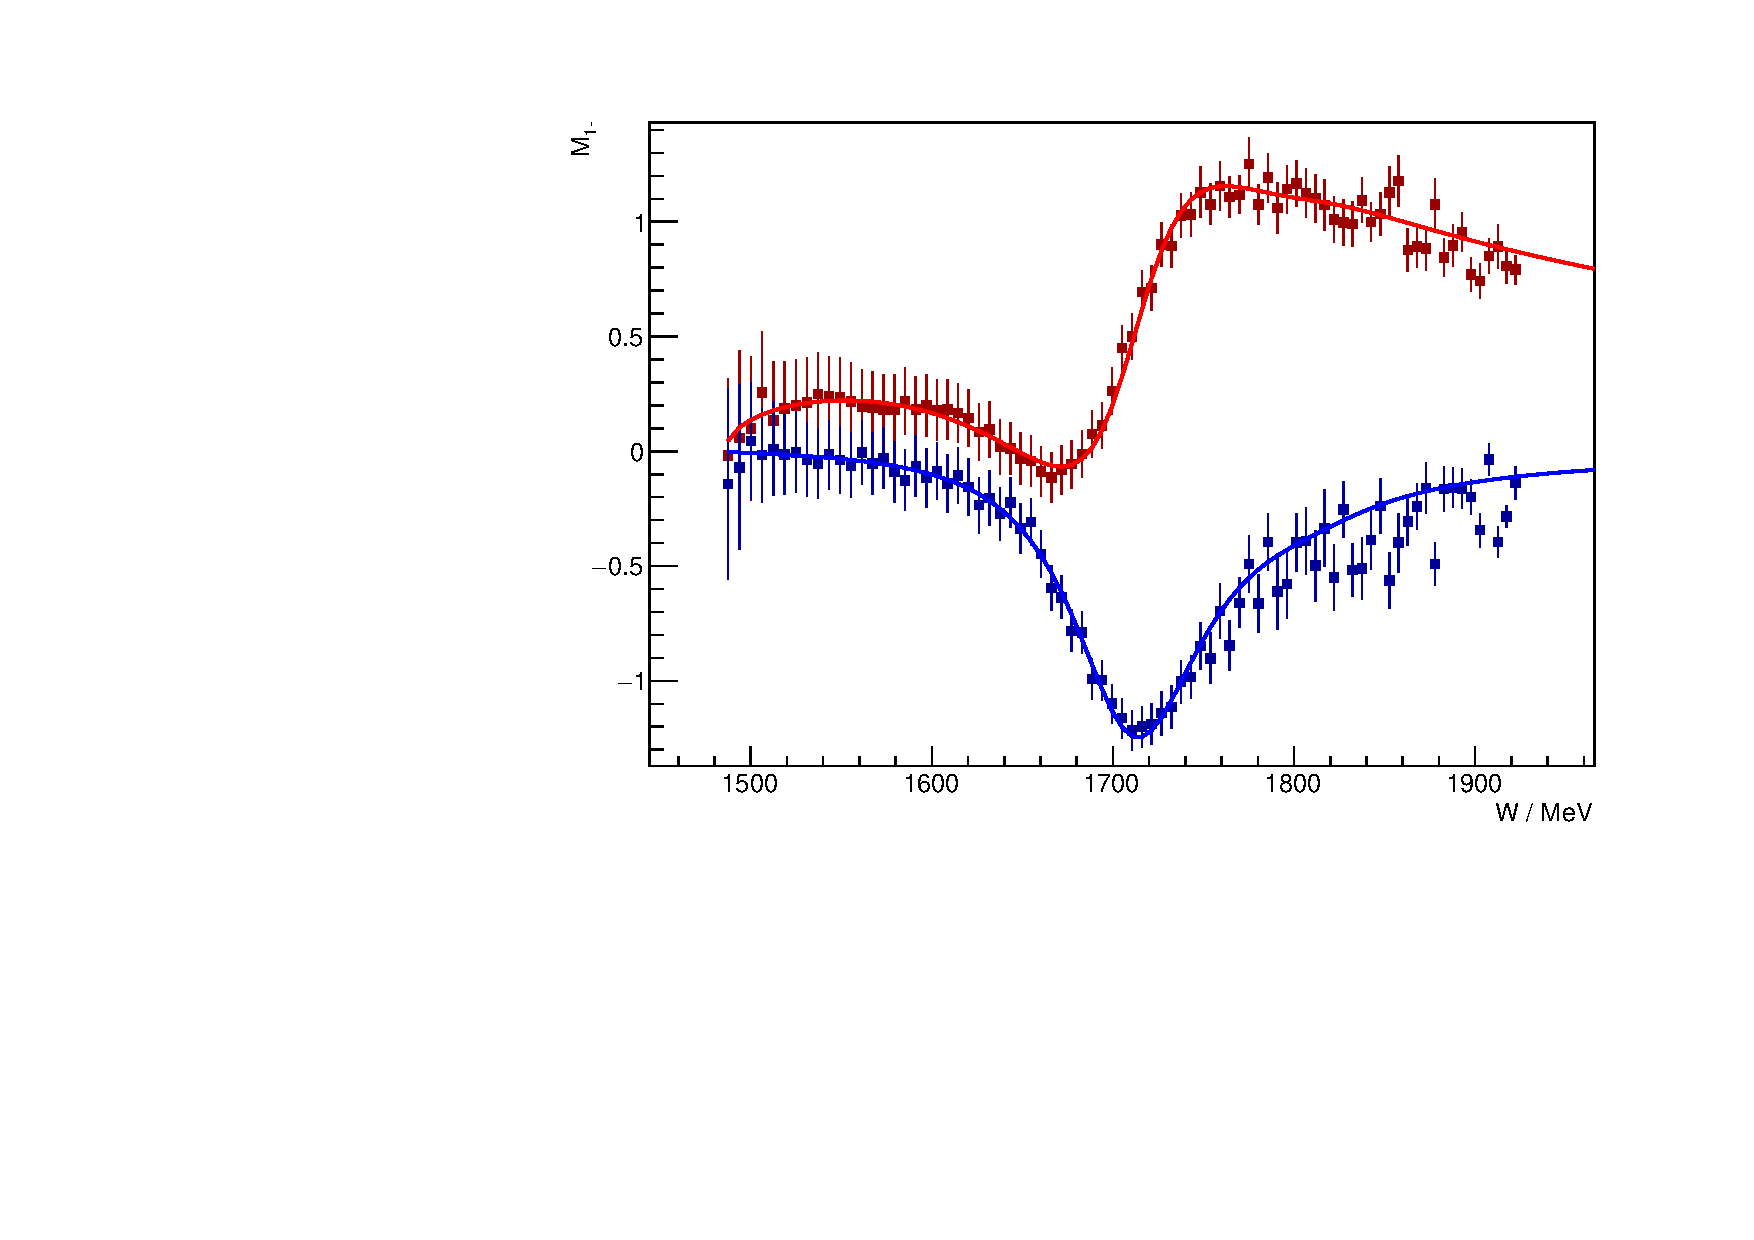
\includegraphics[width=0.49\textwidth]{MAID2015a/Hedim/plots.0/M1m.pdf}
    }
    \centerline{
    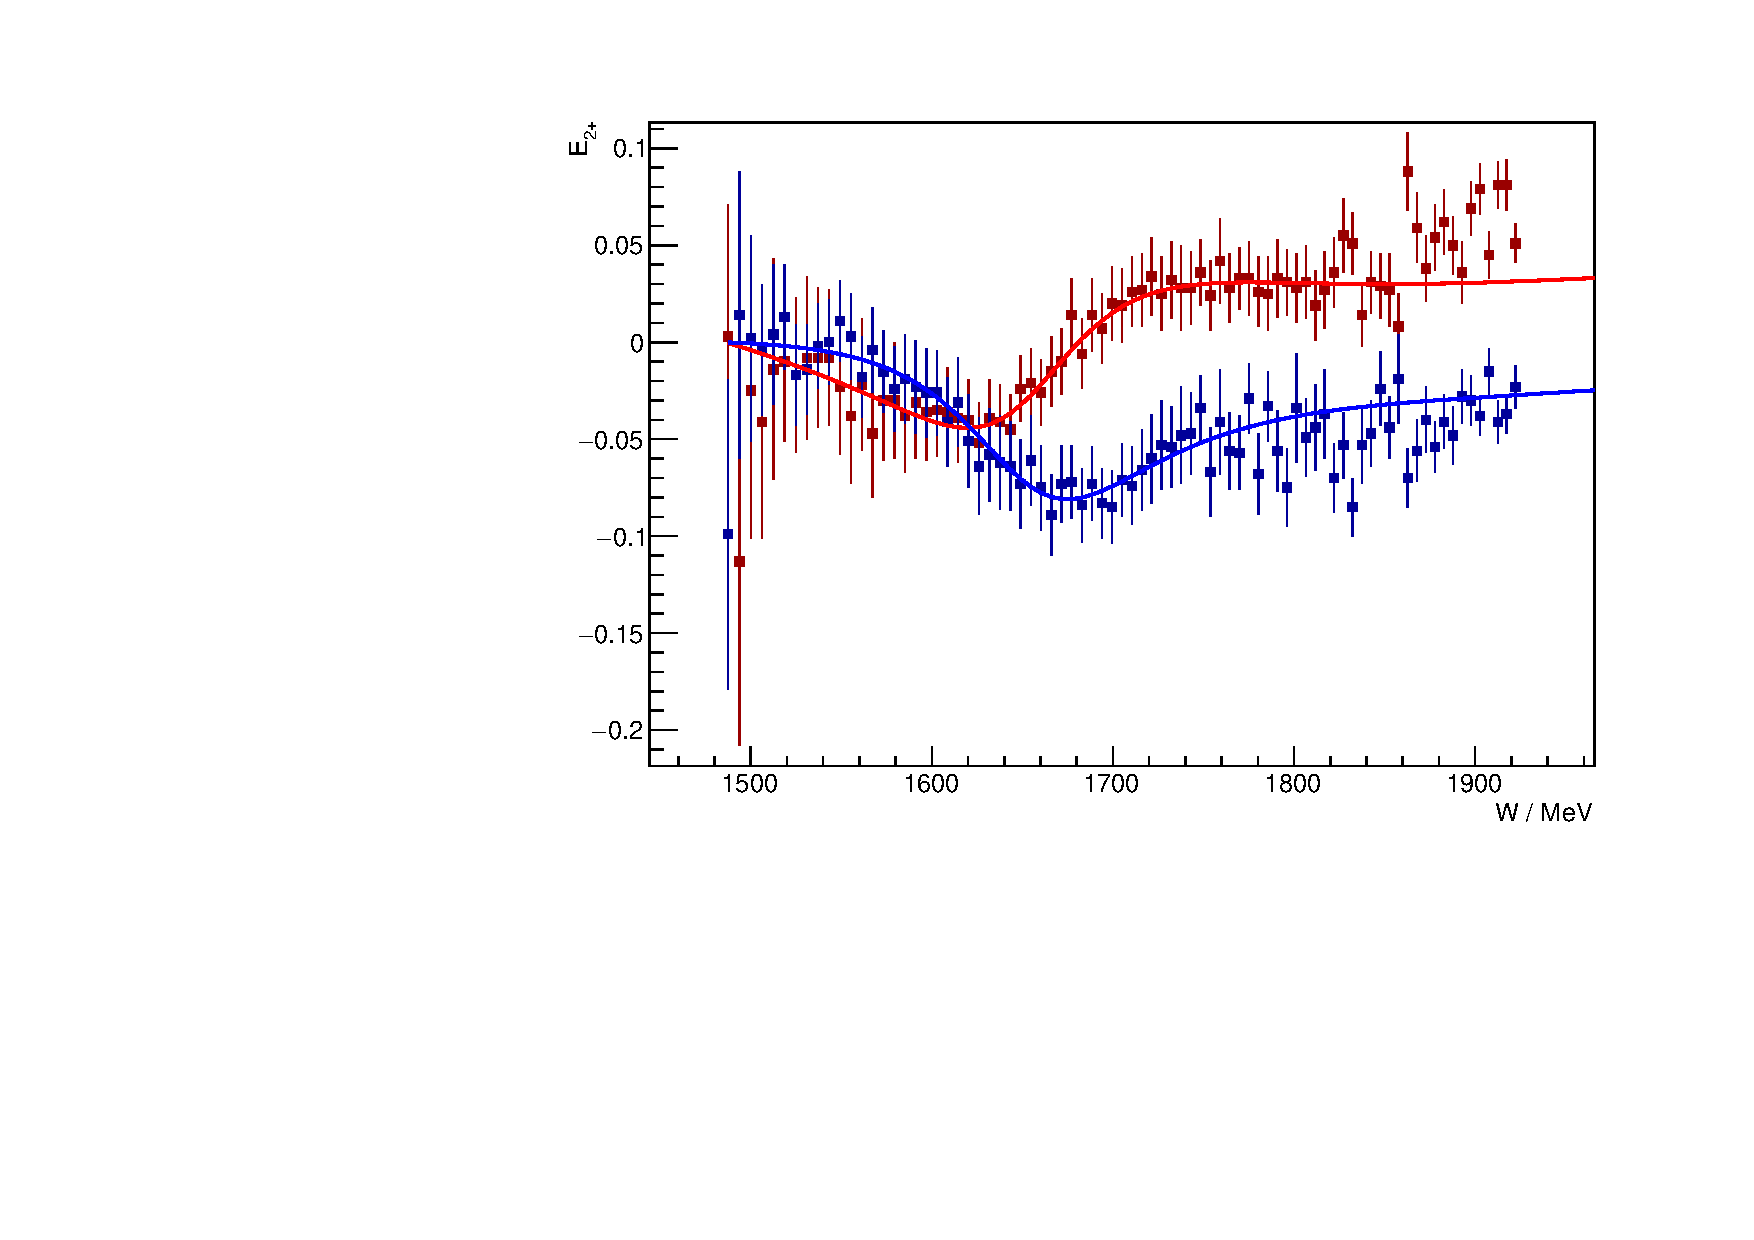
\includegraphics[width=0.49\textwidth]{MAID2015a/Hedim/plots.0/E2p.pdf}
    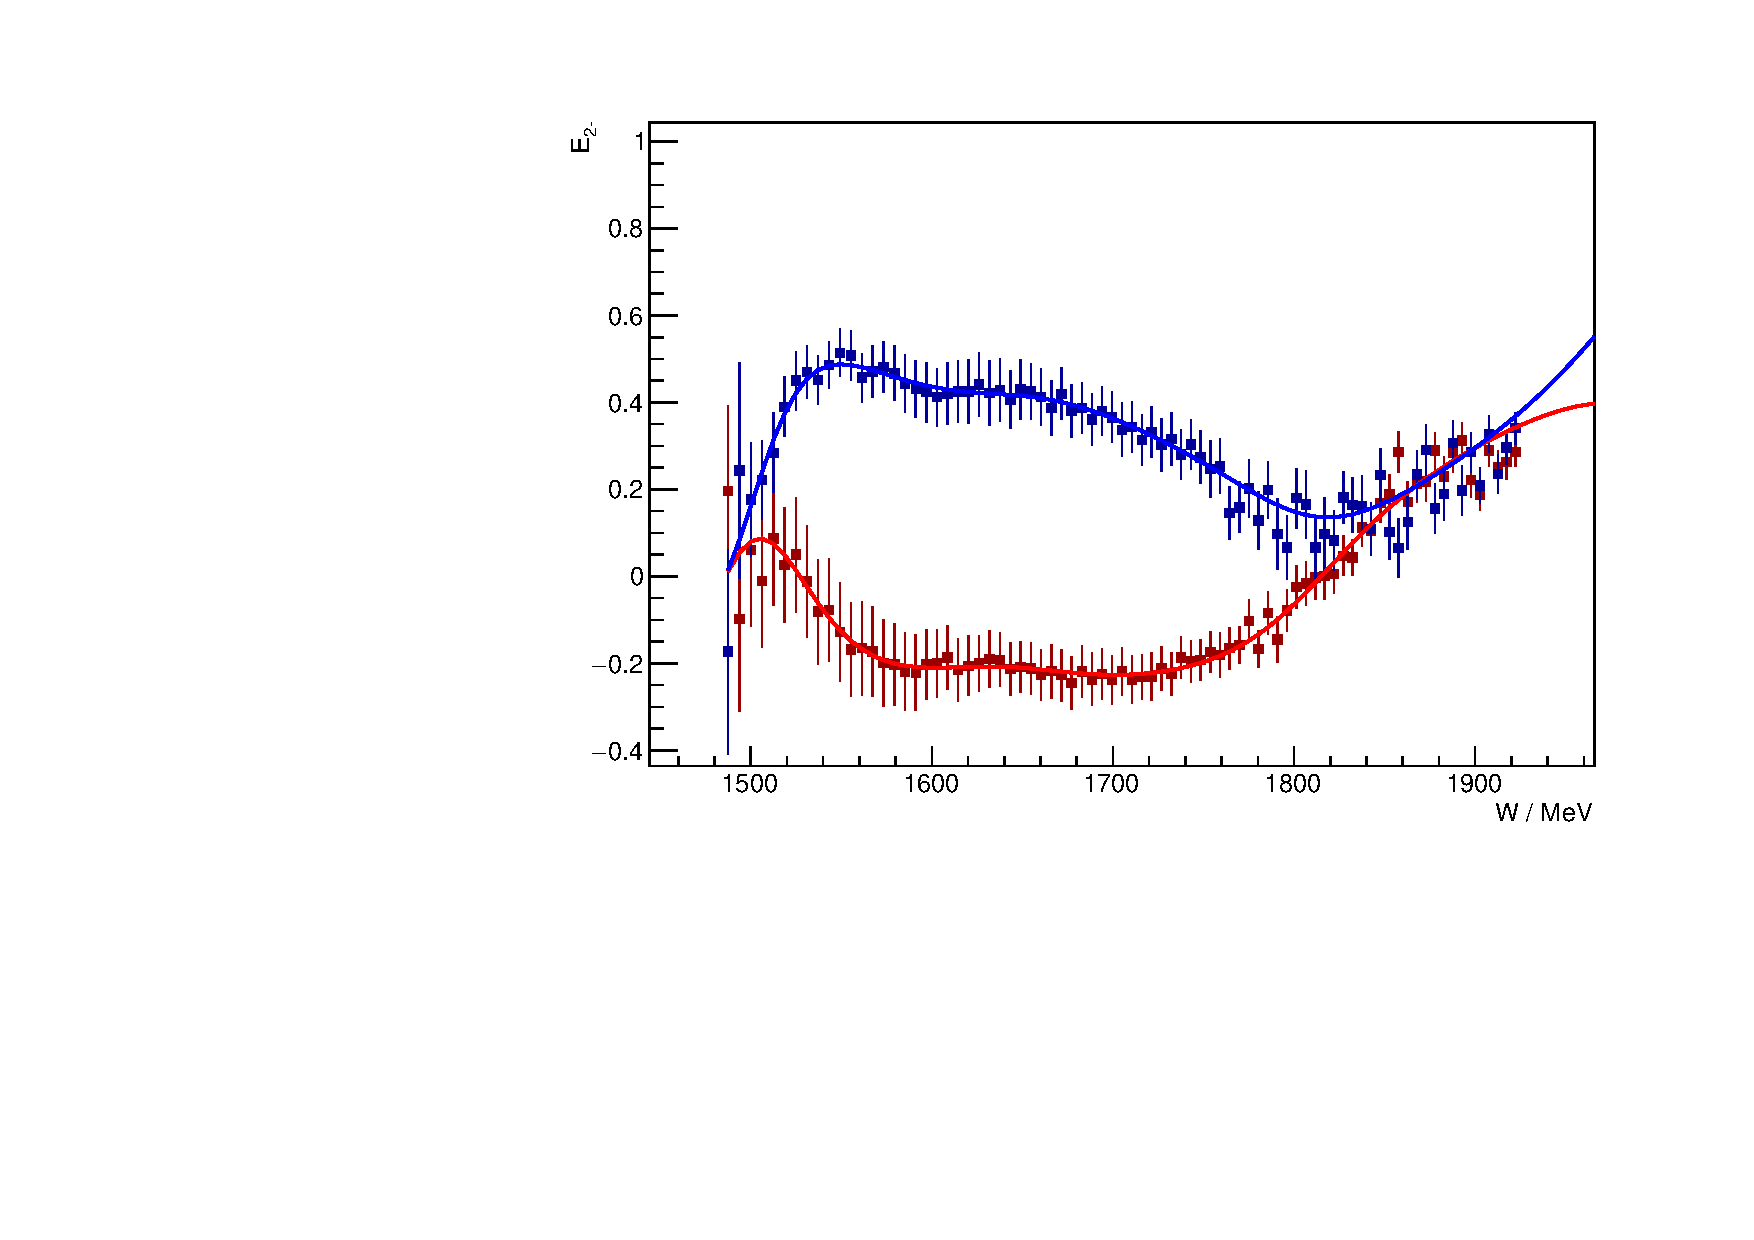
\includegraphics[width=0.49\textwidth]{MAID2015a/Hedim/plots.0/E2m.pdf}
    }
    \centerline{
    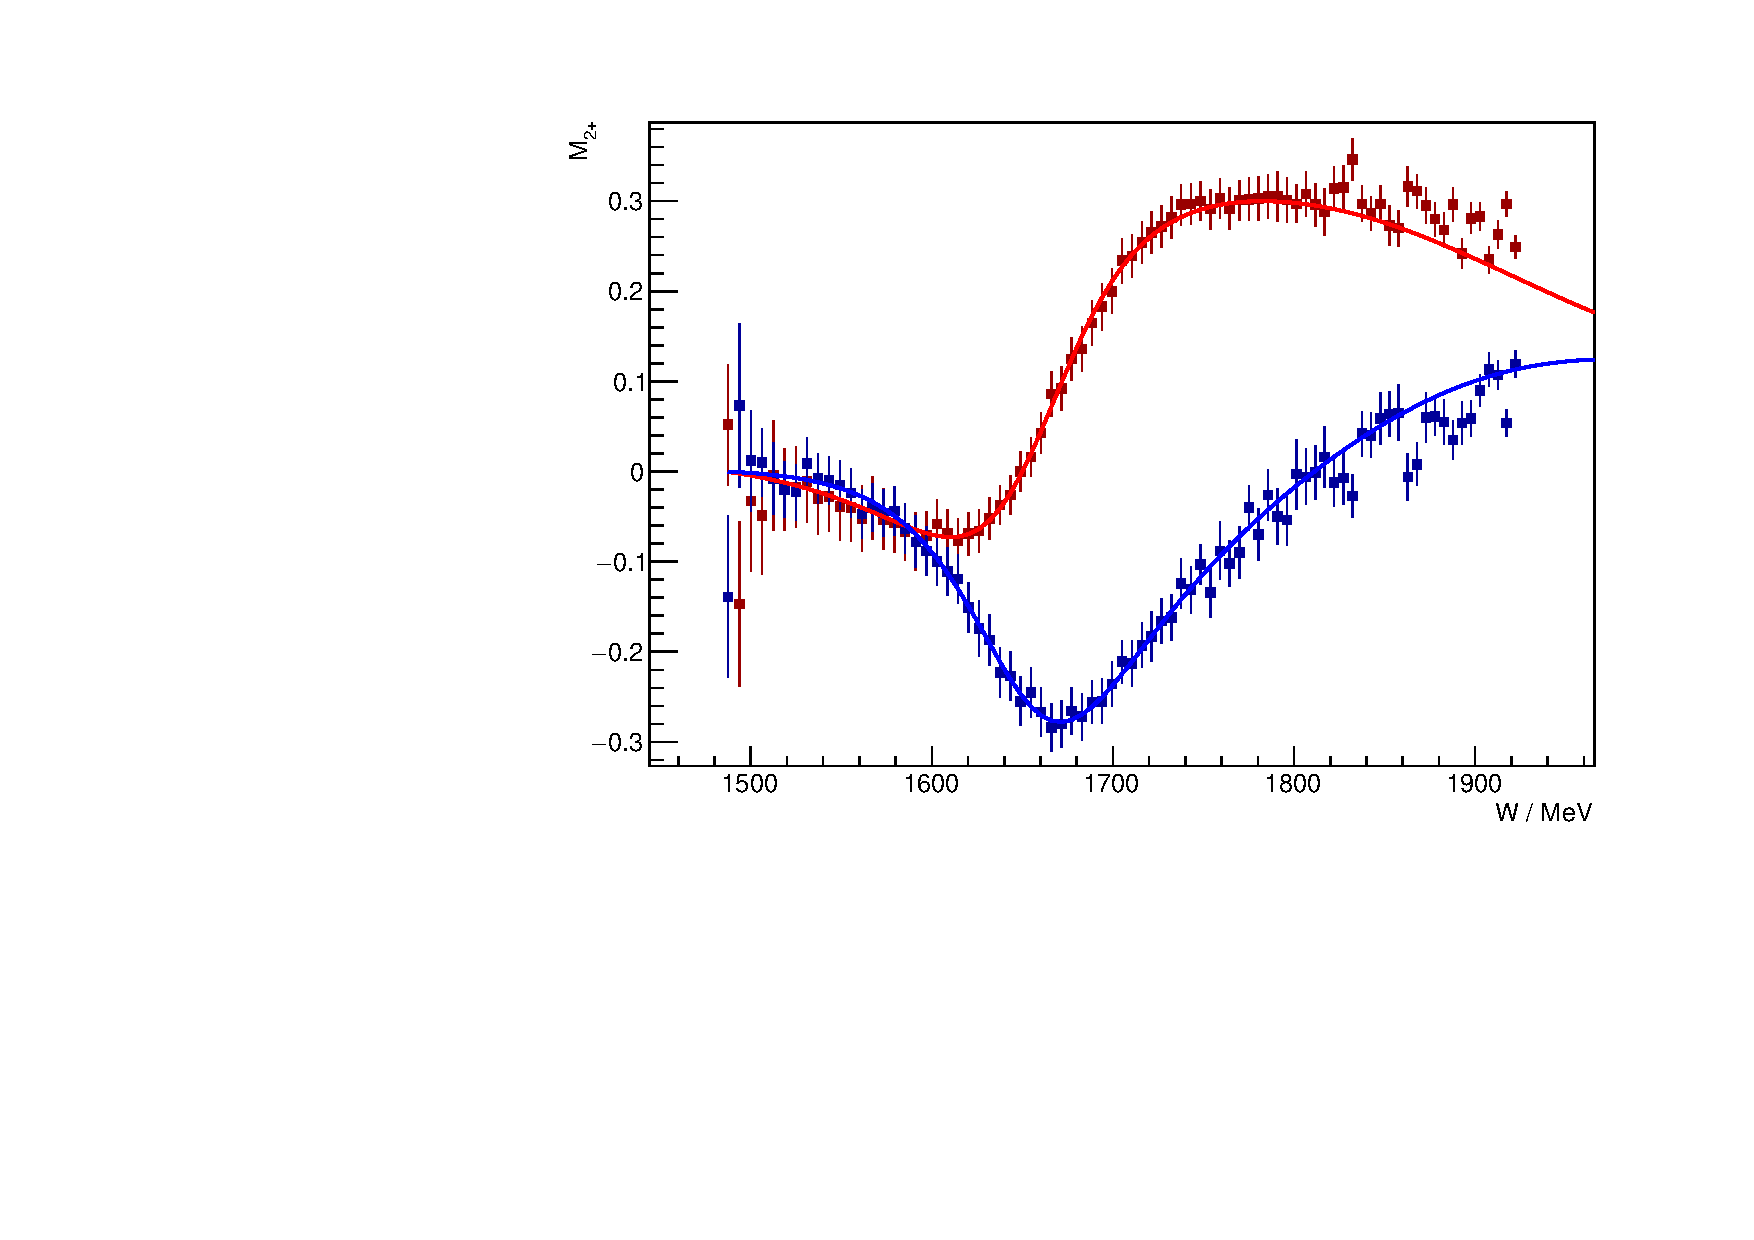
\includegraphics[width=0.49\textwidth]{MAID2015a/Hedim/plots.0/M2p.pdf}
    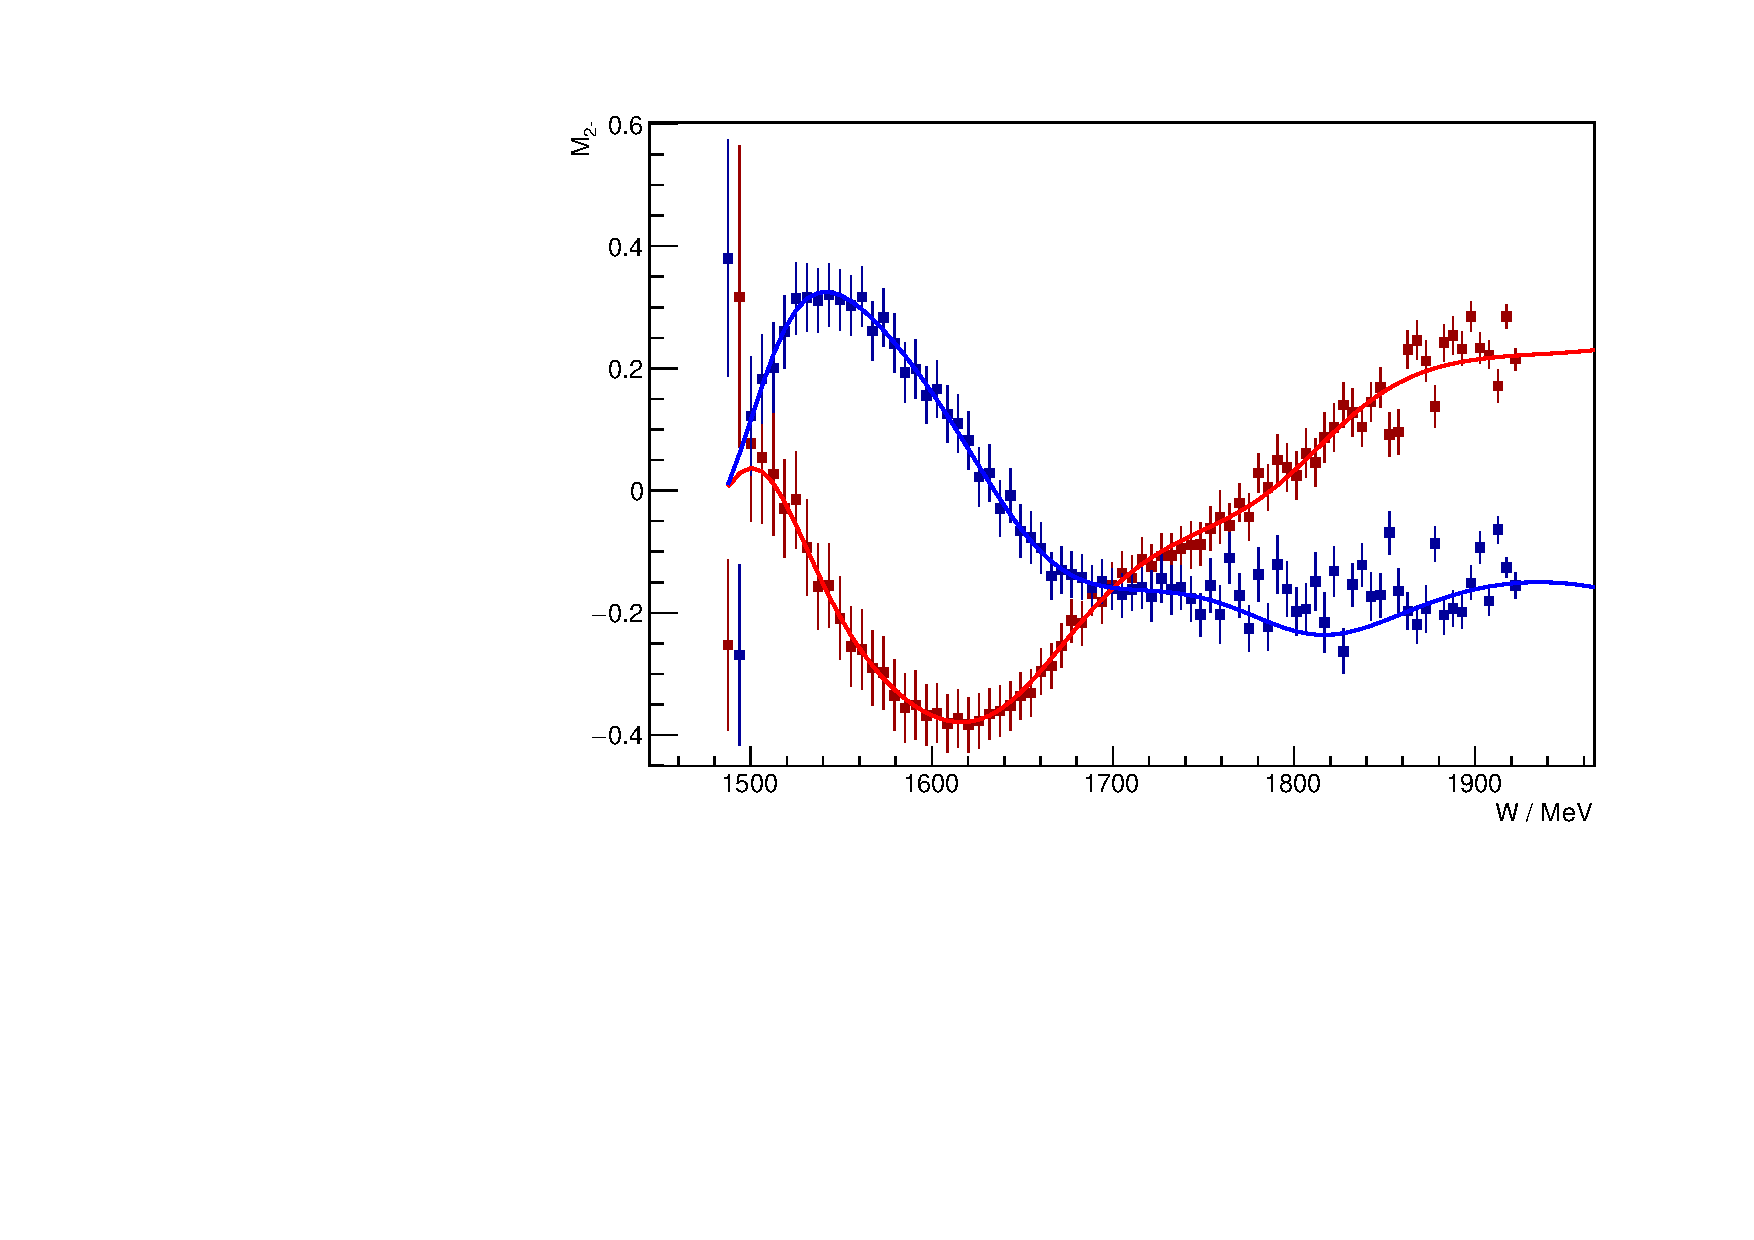
\includegraphics[width=0.49\textwidth]{MAID2015a/Hedim/plots.0/M2m.pdf}
    }
    \caption{s-, p- and d-wave multipoles from a fit constrained to the Hedims amplitudes. 
    Starting values: 50\% range around the MAID15a solution.}
\label{Fig:const4}
  \end{center}
\end{figure}

\begin{figure}
  \begin{center}
    \centerline{
    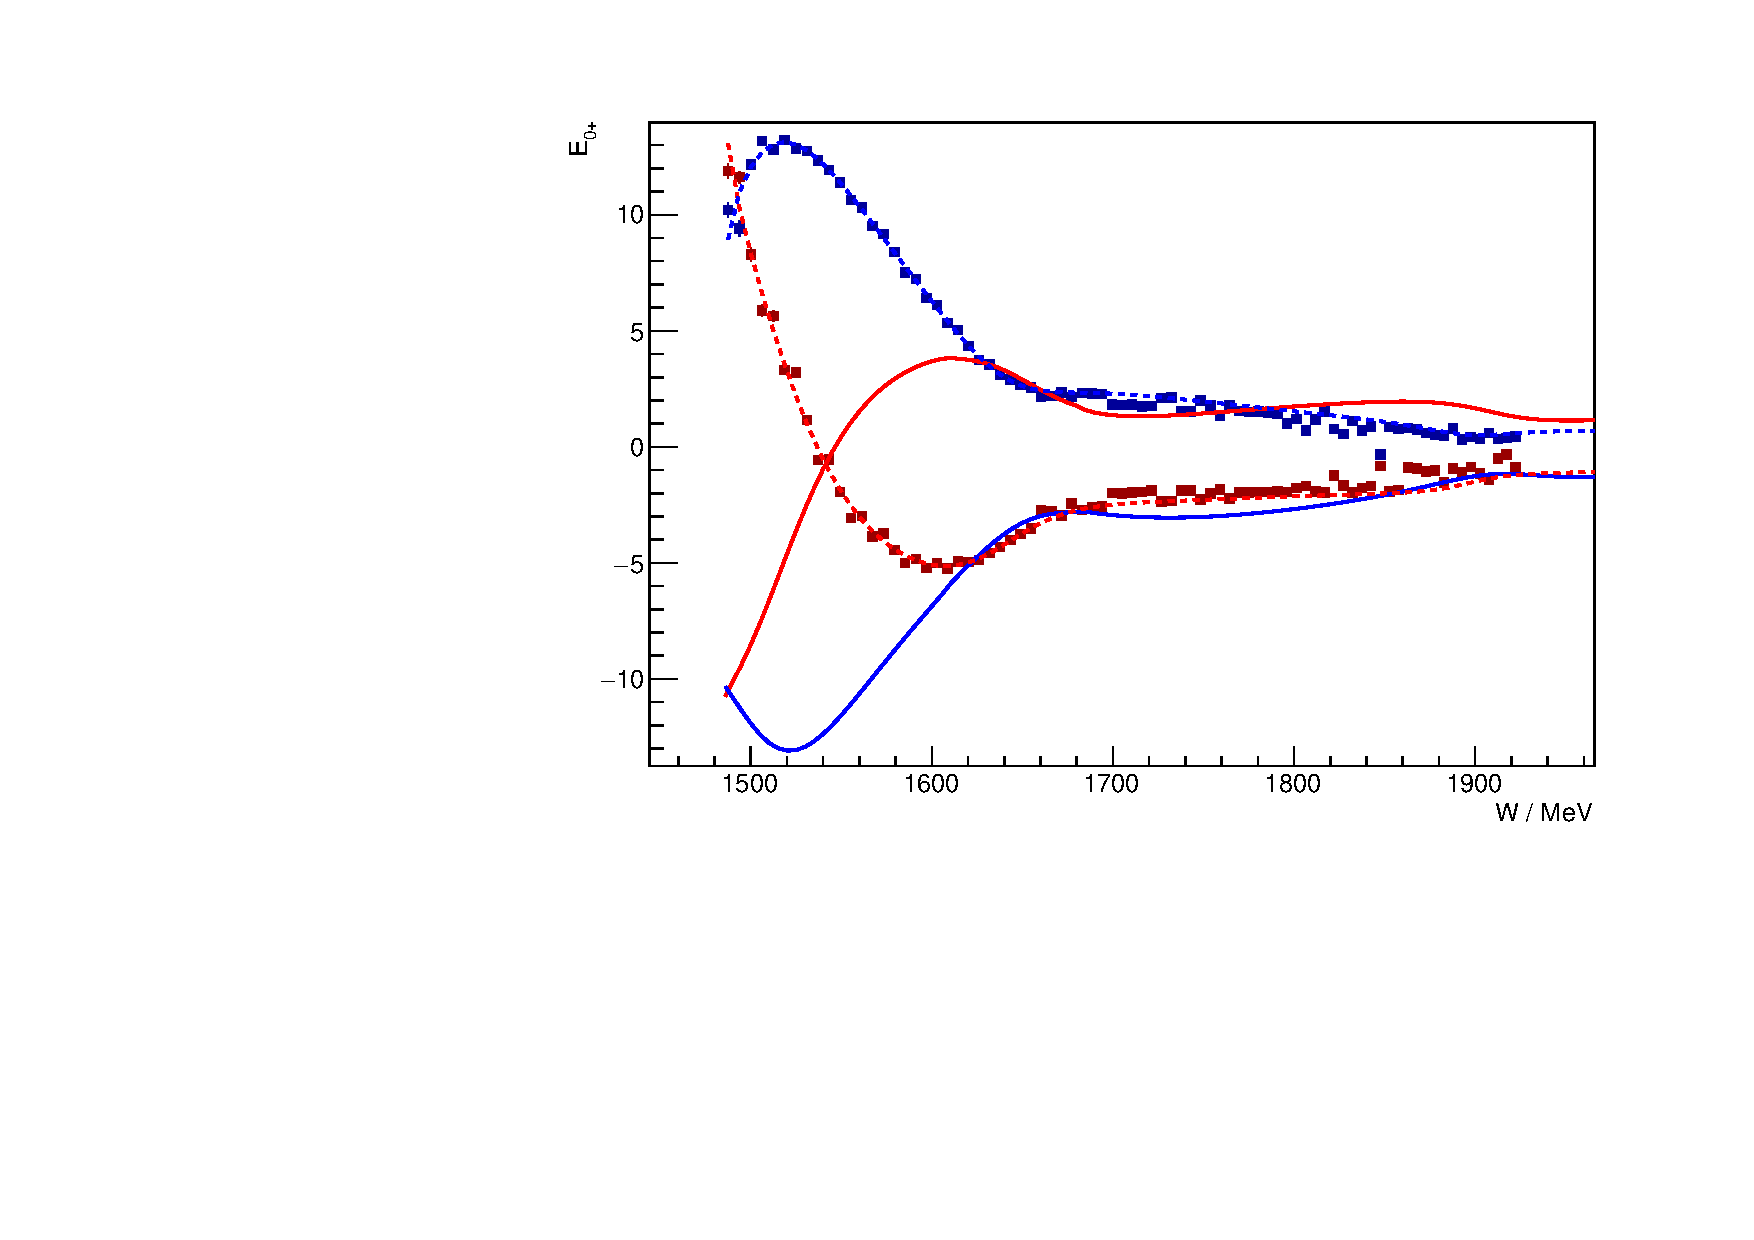
\includegraphics[width=0.49\textwidth]{BnGa/Hedim/plots.0/E0p.pdf}
    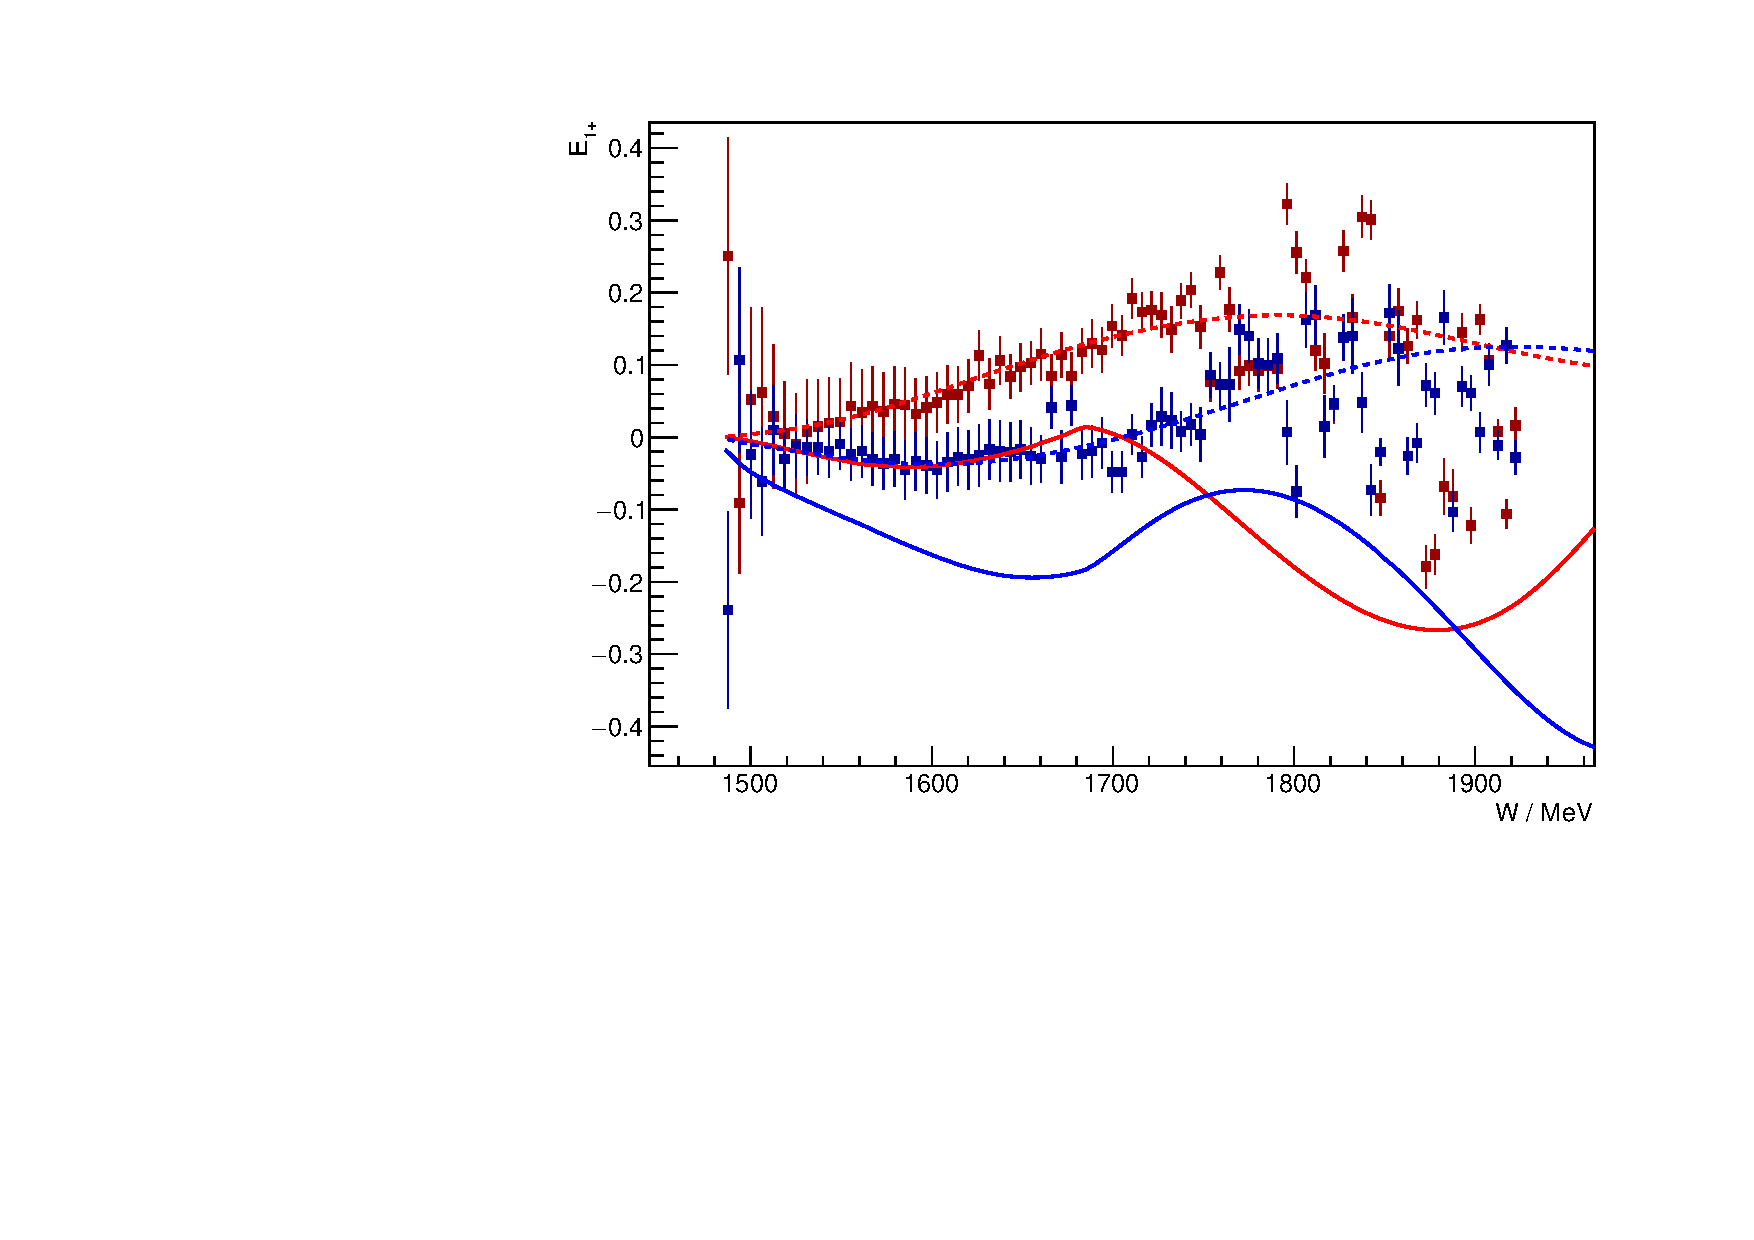
\includegraphics[width=0.49\textwidth]{BnGa/Hedim/plots.0/E1p.pdf}
    }
    \centerline{
    \includegraphics[width=0.49\textwidth]{BnGa/Hedim/plots.0/M1p.pdf}
    \includegraphics[width=0.49\textwidth]{BnGa/Hedim/plots.0/M1m.pdf}
    }
    \centerline{
    \includegraphics[width=0.49\textwidth]{BnGa/Hedim/plots.0/E2p.pdf}
    \includegraphics[width=0.49\textwidth]{BnGa/Hedim/plots.0/E2m.pdf}
    }
    \centerline{
    \includegraphics[width=0.49\textwidth]{BnGa/Hedim/plots.0/M2p.pdf}
    \includegraphics[width=0.49\textwidth]{BnGa/Hedim/plots.0/M2m.pdf}
    }
    \caption{s-, p- and d-wave multipoles from a fit constrained to the Hedims amplitudes. 
    Starting values: 50\% range around the BnGa solution (solid). "True" MAID2015a: dashed.}
\label{Fig:const5}
  \end{center}
\end{figure}

\begin{figure}
  \begin{center}
    \centerline{
    \includegraphics[width=0.49\textwidth]{MAID/Hedim/plots.0/E0p.pdf}
    \includegraphics[width=0.49\textwidth]{MAID/Hedim/plots.0/E1p.pdf}
    }
    \centerline{
    \includegraphics[width=0.49\textwidth]{MAID/Hedim/plots.0/M1p.pdf}
    \includegraphics[width=0.49\textwidth]{MAID/Hedim/plots.0/M1m.pdf}
    }
    \centerline{
    \includegraphics[width=0.49\textwidth]{MAID/Hedim/plots.0/E2p.pdf}
    \includegraphics[width=0.49\textwidth]{MAID/Hedim/plots.0/E2m.pdf}
    }
    \centerline{
    \includegraphics[width=0.49\textwidth]{MAID/Hedim/plots.0/M2p.pdf}
    \includegraphics[width=0.49\textwidth]{MAID/Hedim/plots.0/M2m.pdf}
    }
    \caption{s-, p- and d-wave multipoles from a fit constrained to the Hedims amplitudes. 
    Starting values: 50\% range around the $\eta$-MAID2003 solution (solid). "True" MAID2015a: dashed.}
\label{Fig:const6}
  \end{center}
\end{figure}


\end{document}
